%%%%%%%%%%%%%%%%%%%%%%%%%%%%%%%%%%%%%%%%%%%%%%%%%%%%%
%			HLAVIČKA								%
%%%%%%%%%%%%%%%%%%%%%%%%%%%%%%%%%%%%%%%%%%%%%%%%%%%%%
\documentclass[openany,12pt]{memoir}
\usepackage[utf8]{inputenc} 
\usepackage[czech]{babel}
\usepackage[T1]{fontenc}
\usepackage[top=1cm, bottom=2cm, left=2cm, right=2cm]{geometry}  % --> NASTAVENÍ OKRAJŮ
\usepackage{fancyhdr}
\usepackage{graphicx}
%\usepackage{lmodern}
\usepackage{tgschola}  % --- Silnější font
\usepackage{xwatermark}
\usepackage{xcolor}
\usepackage{changepage}
\usepackage{pdfpages}
\usepackage{lettrine}
\chapterstyle{veelo}  %ALT BIANCHI, veelo



%%%%%% Package na zpěvník
\usepackage[full]{leadsheets}%http://mirrors.nic.cz/tex-archive/macros/latex/contrib/leadsheets/leadsheets_en.pdf   --> dokumentace	
\definesongtitletemplate{empty}{} 
\setchords{
format = \bfseries,   %tučné akordy
minor = {mi},% 
input-notation = {german},%
output-notation = {german}%
}
\definesongtitletemplate{empty}{} 

\newlength{\drop}
\newwatermark[pages=3-,color=red!50,angle=0,scale=2, xpos=0,ypos=0]{
\includegraphics[width=5cm]{obr/pozadi2.jpg}} %--> dvojka na pozadí


%%%% Vlastní příkazy
\newcounter{Slokočet}   %Automatické číslování slok
\newcommand{\mezera}{\vspace*{0.5cm}}   %Horizontální odsazení slok
\newcommand{\stred}{5.2cm}   %%% Na zarovnání slok doprostřed, pozn. automatičtější zarovnávání na střed nejde
\newcommand{\refren}{\mezera \noindent \textbf{R:} } %refrén
\newcommand{\sloka}{\mezera \noindent \addtocounter{Slokočet}{1} \arabic{Slokočet}. } 	%sloka, která se automaticky čísluje
\newcommand{\ssloka}{\mezera \noindent}  % vlastní číslo sloky
\newcommand{\carka}{,\:}
\newcommand{\m}[1]{\color{white}{#1}}  %Pro akordy
\newcommand{\ap}{'}	%Pro apostrof


\addto\captionsczech{\renewcommand{\contentsname}{Seznam písní}}


%%%%%%%%%%%%%%%%%%%%%%%%%%%%%%%%%%%%%%%%%%%%%%%%%%%%%%
%			NÁVOD									 %
%%%%%%%%%%%%%%%%%%%%%%%%%%%%%%%%%%%%%%%%%%%%%%%%%%%%%%
%1. Věci v hlavičce IGNOROVAT
%2. Píseň psát do prostoru mezi \begin{song} a \end{song}
%3. další řádek se značí dvěma odsazeníma (= dvakrát stisknout enter)
%4. \refren vždy na začátku refrenu a \sloka na začátek sloky (automaticky se čísluje)
%  \ = alt gr + q ; [/] = alt gr f/g ; {/} = alt gr + b/n; ^ = alt gr + 3 + mezera
%Cokoliv napíšete do ^{  } se bude brát jako akord
%když se toto bude dotýkat nějakého slova (nebude mezi tím a slovem mezera)
%tak se akordy zjeví nad slovem, ale pište to před slovo
%Když se to nedotýká slova, tak akord lítá ve vzduchu a vytiskne se větší mezera
%První možnost je asi preferovanější
%5. Akordy stačí psát jen do první sloky, když se nezmění -- kytaristi to zvládnou



%
%\usepackage{subfiles}
%</++>

\begin{document}\renewcommand{\abstractname}{\vspace{-\baselineskip}}
%Kompilovat dvakrát, aby se updatnula TOC
\pagestyle{empty}
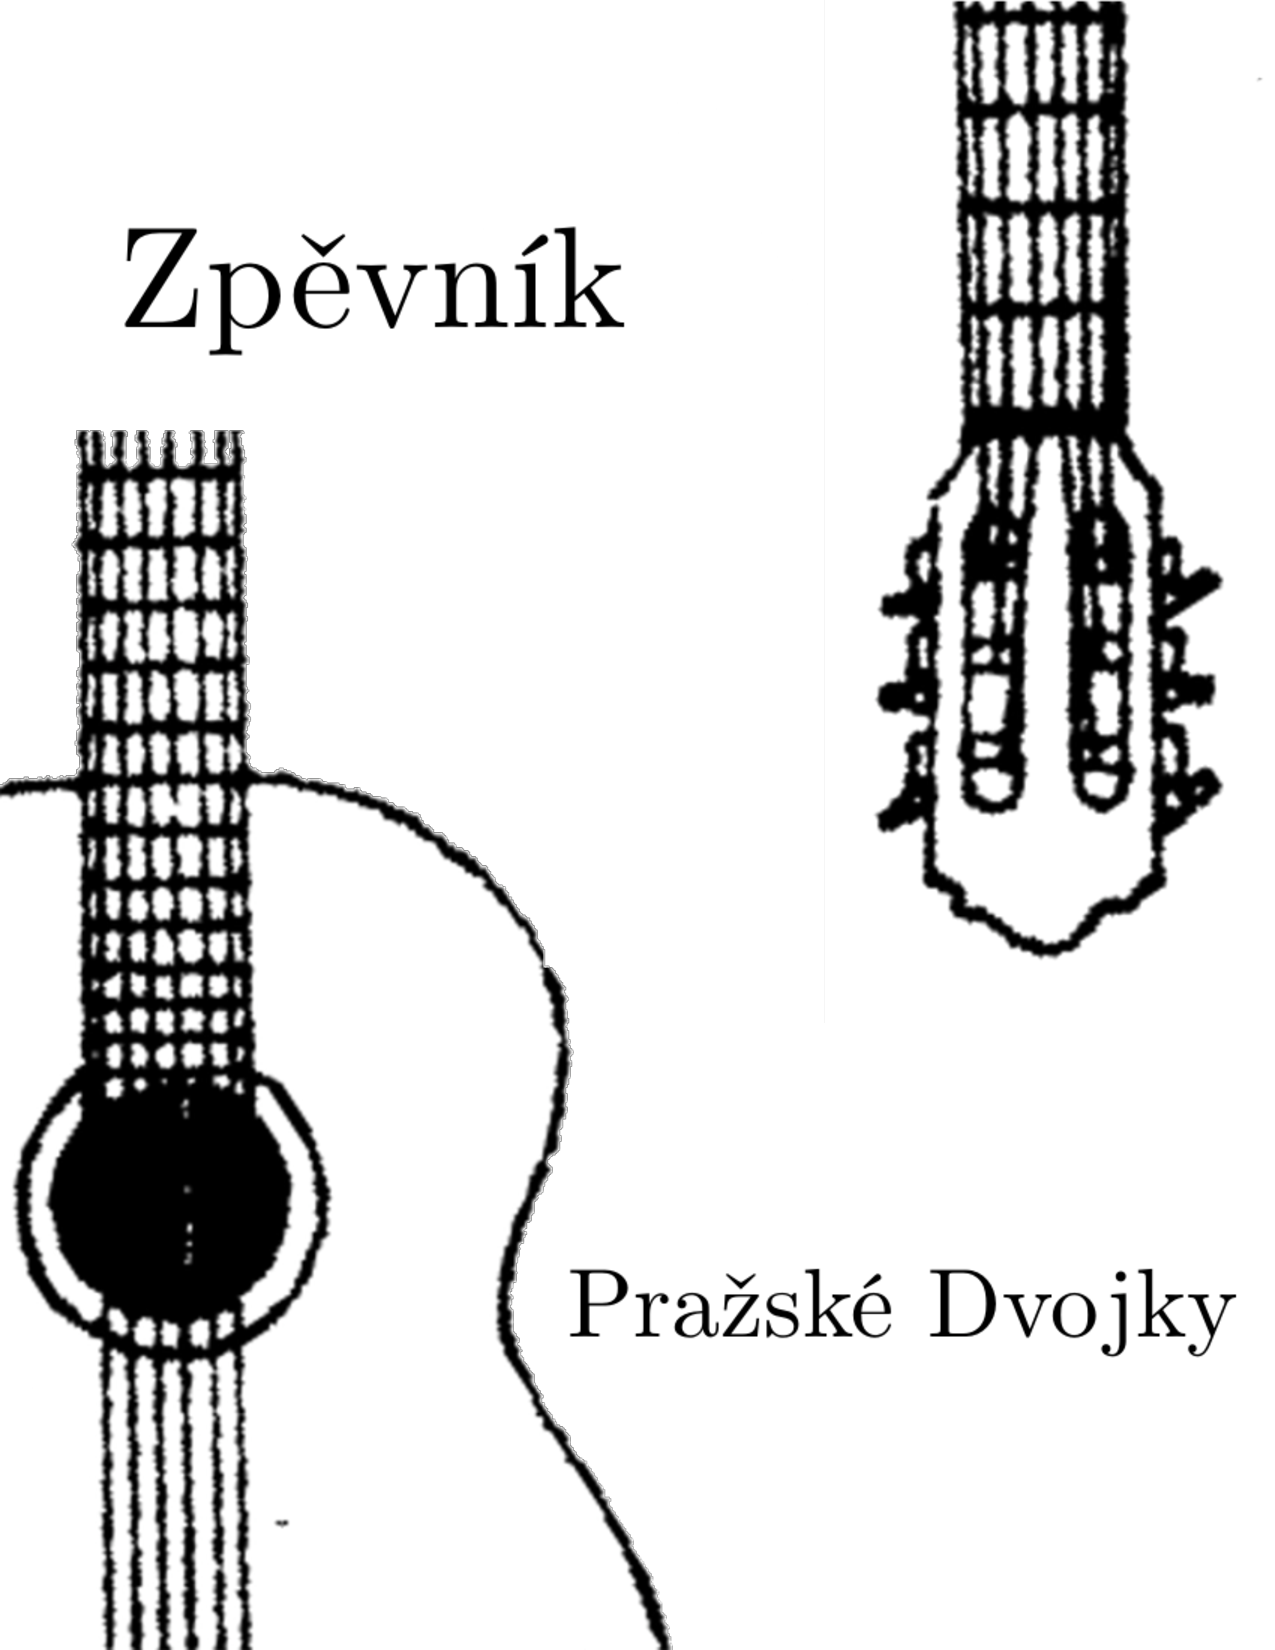
\includepdf{obr/cover3}

\newpage
	
\setcounter{page}{1}
\vspace*{4\baselineskip}
\begin{abstract}
\large
\lettrine{P}{rávě} se k Vám dostal další z řady oddílových zpěvníků \textbf{Pražské Dvojky}.
Tento zpěvník si klade za cíl se od svých předchůdců odlišovat a být striktně lepší 
náhradou poskytující všemožné designové a funkční vylepšení. Navíc, díky psaní tohoto 
zpěvníku v~programu \LaTeX \,, dosahuje značné flexibility a při případných přípravách nové verze zpěvníku 
stačí upravit tento zpěvník a není nutné začínat od znova.\\
Najdete tu značné množství písniček, které tvůrci považují za hodící se k ohni s~kytarou, 
akordy na ně a to vše v moderním provedení. Doufáme, že Vám tento zpěvník pomůže k~dosažení 
správné táborákové atmosféry a že v něm najdete všechny písničky, které chcete, ale i jiné, 
které se Vám zalíbí a obohatí Vás. V případě, že v něm naleznete nesrovnalosti nebo byste do něj 
chtěli přidat další píseň, rádi Vaše připomínky zapracujeme do budoucích verzí zpěvníku.\\\\\\\\\\
Hodně zábavy při zpěvu přejí tvůrci zpěvníku:\\\\
$\mathcal{J}$indra \& $\mathcal{A}$lbert\\\\\\\\\\\\\\\\\\\\\\\\
{\tiny Zpěvník 18.06, Aranžovaná anakonda LTS  } %Ubuntu roleplay
\end{abstract}
\newpage

%\addtocontents{toc}{\protect\thispagestyle{empty}}
\tableofcontents* \thispagestyle{empty}\newpage
\newgeometry{top=1.5cm, bottom = 0cm, left = 2cm, right = 2cm}

\pagestyle{simple}
\addcontentsline{toc}{section}{Skautská hymna a Večerka}%\documentclass[../main.tex]{subfiles}

\begin{song}{title=\centering Skautská hymna \\\normalsize  \vspace*{-0.3cm}}  %% sem se napíše jméno songu a autor
\moveright 6cm \vbox{      %Varianta č. 1  ---> Jeden sloupec zarovnaný na střed	
\textcolor{white}{something}


^{D}Junáci ^{G}vzhůru, ^{D}volá den,

luh ^{Hmi}květem ^{G}kývá, ^{A}orosen,

sluníčko blankytem pílí,

před ^{Emi}námi pouť ^{F#m}vede k ^{A}cíli.

^{D}Junáci ^{G}vzhůru ^{D}volá den,

^{G}junáci ^{D G}vzhůru ^{A}volá ^{D}den. 

}
\setcounter{Slokočet}{0}
\end{song}

\vspace*{7cm}
\begin{song}{title=\centering Večerka \vspace*{-0.3cm}}
\moveright 6.2cm \vbox{      %Varianta č. 1  ---> Jeden sloupec zarovnaný na střed	

\sloka
 Zapad den, slunce svit,
 
 vymizel z údolí,
 
 z temen hor odpočiň
 
 každý kdos boží tvor.
 
\sloka
 V lese klín padl stín,
 
 hasne již vatry zář,
 
 svatý mír kráčí z hor,
 
 usíná boží tvor.
 
\sloka
BRUMENDO
}
\setcounter{Slokočet}{0}
\end{song}

\newpage
\addcontentsline{toc}{section}{1. signální}\begin{song}{title=\centering 1. signální \\\normalsize Chinaski  \vspace*{-0.3cm}}  %% sem se napíše jméno songu a autor
\moveright \stred \vbox{      %Varianta č. 1  ---> Jeden sloupec zarovnaný na střed	

\sloka 
	^{Emi}Až si ^{G}zejtra ráno ^{C}řeknu zase 

	^{Emi}jednou provždy dost,

	^{G}právem se mi ^{C}budeš tiše ^{Emi}smát

	jak omluvit si svoji slabost,

	nenávist a zlost,

	když za všechno si můžu vlastně sám. 

\refren
	^{Ami}Za spoustu dní možná za ^{C}spoustu let 

	až se mi ^{G}rozední, budu ti ^{D}vyprávět 

	na 1.signální, jak jsem vobletěl svět, 

	jak tě to vomámí a nepustí zpět.

	Jaký si to ^{F}uděláš, ^{B}takový to ^{Dmi}máš. 

	Jaký si to ^{F}uděláš, ^{B}takový to ^{Dmi}máš. 

\sloka
	Až se dneska večer budu tvářit
	
	zas jak Karel Gott, 
	
	budu zpívat vampamtydapam,
	
	všechna sláva polní tráva,
	
	ale peníz přijde vhod,
	
	jak jsem si to uďál tak to mám.

\refren

\sloka Nana\dots

}
\setcounter{Slokočet}{0}
\end{song}


\newpage
\addcontentsline{toc}{section}{Always Look On The Bright Side Of Life}\begin{song}{title=\centering Always Look On The Bright Side Of Life \\\normalsize Monty Python  \vspace*{-0.3cm}}  %% sem se napíše jméno songu a autor
\moveright 3.3cm \vbox{      %Varianta č. 1  ---> Jeden sloupec zarovnaný na střed	

\sloka 
	Some ^{Ami}things in life are ^{D}bad, they can ^{G}really make you ^{Emi}mad.

	Other ^{Ami}things just make you ^{D}swear and ^{G}curse.

	When you've ^{Am}chewing on life's ^{D}gristle, don't ^{G}grumble give a ^{Emi}whistle.

	And ^{Ami}this'll help things turn out for the ^{D7}best.

\refren
	And ^{G}always ^{Emi}look on the ^{Ami}bright ^{D7}side of ^{G}life ^{Emi\,Ami\,D7}.

	Always look on the light side of life.

\sloka
	If ^{Ami}life seems jolly ^{D}rotten, there's ^{G}something you've ^{Emi}forgotten.

	and that's to ^{Ami}laugh and smile and ^{D}dance and ^{G}sing.
	
	When you've ^{Ami}feeling in the ^{D}dumps don't, be ^{G}silly ^{Emi}chumps.

	Just ^{Ami}purse your lips and whistle -- that's the ^{D7}thing.

\refren
	And always look on the bright side of life

	Come on always look on the bright side of life


\sloka
	For life is quite absurd and death's the final word,

	you must always face the curtain with a bow.

	Forget about your sin -- give the audience a grin.

	Enjoy it -- it's your last chance anyhow.


\refren
	So always look on the bright side of death
	
	just before you draw your terminal breath

\sloka
	Life's a piece if shit when you look at it.

	Life's a laugh and death's a joke it's true.

	You'll see it's all a show, keep'em laughing as you go.

	Just remember that the last laugh is on you.

\refren
	And always look on the bright side of life
	
	Always look on the right side of life
	
	(Come on guys, cheer up)


/: ^{A}Always ^{F#}look on the ^{Hmi}right ^{E7}side of ^{A}life ^{F#\,Hmi\,E7} :/




}
\setcounter{Slokočet}{0}
\end{song}
\newpage
\addcontentsline{toc}{section}{Amerika}\begin{song}{title=\predtitle \centering Amerika \\\large Lucie  \vspace*{-0.3cm}}  %% sem se napíše jméno songu a autor
\begin{centerjustified}
\nejvetsi
\sloka 
	^{G\z }Nandej mi ^{D}do hlavy tvý ^{Ami\z }brouky 
	
	a Bůh nám seber ^{\z G}beznaděj.
	
	V duši zbylo ^{D\z }světlo z jedný ^{Ami}holky,
	
	tak mi teď za to ^{\z G}vynadej.
	
	Zima a ^{D\z }promarněný ^{Ami}touhy, 
	
	do vrásek stromů padá ^{G}déšť. 
	
	Zbejvaj roky ^{D}asi ne moc ^{Ami}dlouhý.
	
	Do vlasů mi ^{\z C}zabroukej pá pa pá ^{G}pá. 

\refren
/: Pá ^{G/F#}pá pa ^{Emi\z}pá,~pá pa pa ^{G}pá. :/

\sloka
	Tvoje oči jenom žhavý tóny, 
	
	dotek slunce zapadá.
	
	Horkej vítr rozezní mý zvony.
	
	Do vlasú ti zabrouká pá pa pa pá. 

\refren

\sloka
	Na obloze křídla tažnejch ptáků,
	
	tak už na svý bráchy zavolej. 
	
	Na tváře ti padaj slzy z mraků
	
	a Bůh nám sebral beznaděj. 
	
	V duši zbylo světlo z jedný holky,
	
	do vrásek stromů padá déšť. 
	
	Poslední dny hodiny a roky, 
	
	do vlasů ti zabrouká pá pa pa pá.

\refren


\end{centerjustified}
\setcounter{Slokočet}{0}
\end{song}


\newpage
\addcontentsline{toc}{section}{Anděl}\begin{song}{title=\predtitle \centering Anděl \\\large Karel Kryl   \vspace*{-0.3cm}}  %% sem se napíše jméno songu a autor
\begin{centerjustified}
\nejnejvetsi
\sloka 
	^{G}Z ^{\z Emi}rozmlácenýho kostela ^{G\z}v~krabici ^{D7\z}s~kusem mýdla

	^{G\z}přinesl ^{Emi}jsem si anděla, ^{G\z D7}polámali mu křídla.

	Díval se na mě oddaně, já měl jsem trochu trému,

	tak vtiskl jsem mu do dlaně lahvičku od parfému.

\refren
	^{G\z}A~proto, ^{Emi\z }prosím, věř mi, ^{G\z}chtěl jsem ho ^{D7\z}žádat,
	
	^{G}aby mi ^{Emi\z }mezi dveřmi ^*{G}po mohl ^*{D7}hád at,

	^{G}co mě čeká ^{Emi} ^{D}a nemine, ^{G}co mě čeká ^{Emi} ^{D7}a  ^*{\z G}nemine .

\sloka
	Pak hlídali jsme oblohu, pozorujíce ptáky,
	
	debatujíce o Bohu a hraní na vojáky.

	Do tváře jsem mu neviděl, pokoušel se ji schovat,

	to asi ptákům záviděl, že mohou poletovat.

\refren

\sloka
	Když novinky mi sděloval u okna do ložnice,

	já křídla jsem mu ukoval z mosazný nábojnice,
	
	a tak jsem pozbyl anděla, on oknem odletěl mi,

	však přítel prý mi udělá novýho z mojí helmy.

\refren

\end{centerjustified}
\setcounter{Slokočet}{0}
\end{song}
\newpage
\addcontentsline{toc}{section}{Antidepresivní rybička}\begin{song}{title=\predtitle \centering Antidepresivní rybička \\\large Vypsaná Fixa   \vspace*{-0.3cm}}  %% sem se napíše jméno songu a autor
\begin{centerjustified}
\nejnejvetsi
\begin{varwidth}[t]{0.48\textwidth}\setlength{\parindent}{0.45cm}  %Varianta č. 2 --> Dva sloupce
\sloka 
  ^{C}Ona má ^{Emi}antidepresivní ^{F\z }rybičku

  ^*{C}vy tetovanou na 
  
  ^*{Emi}nejta jnějším ^{F\z }místě.

  Možná je pod srdcem 

  a možná trochu níž.

  Ona může všude,

  prostě tam, kam 
  
  si vymyslíš.

\refren
  A ona ^{C\z }plave 

  z orgánu ^{G}do orgánu.

  Žere ^{Ami\,\,}plevel,

  ^{D\,\,}kterej po ránu

  ^*{C}om otává mozek

  a ^*{G}ko tníky na konci 
  
  ^{\z Ami}pelesti.\phantom{xt}

  ^{D}Hu!


\end{varwidth}\mezisloupci \begin{varwidth}[t]{0.48\textwidth}\setlength{\parindent}{0.45cm}
\vspace*{0.465cm}  % V případě varianty č.2 jde odsud text do pravé části

\sloka
  Veze si antidepresivní rybičku

  městem co má velkou spoustu 
  
  pastí.

  Falešný městský strážník,

  bary a zloděj kol 
  
  a nebo prostě každý, 

  koho si ty 

  vymyslíš.


\refren
 /:  Ona je rebel, 
  
  kouří na zastávce,

  jí to chutná  

  v týhle válce 

  a její vnitřní orgány

  tolerují její rebelství. :/

\sloka 
  /: A potom přijde DJ PUNK,

  bude to nejlepší herec a další 

  a celej underground 

  i ryba pod monopolem. :/

\refren
  A ona plave 
  
  z modřiny do modřiny

  a vygumuje 

  je úplně všechny

  a tvoje vnitřní orgány 

  tolerují její rebelství.

  Hu!



\end{varwidth}
\end{centerjustified}
\setcounter{Slokočet}{0}
\end{song}

\newpage
%Zde je vyhrazené místo, kde nebude Bedna od Whisky
\addcontentsline{toc}{section}{Cestou do Jenkovic}\begin{song}{title=\predtitle\centering Boží Vlak\\\large \vspace*{-0.3cm}}  %% sem se napíše jméno songu a autor
\begin{centerjustified}
\nejnejvetsi
	
\sloka 
	To ^{C\z}boží vlak již jede a míří ^{Ami\z}zrovna ^{G\z}sem.
	
	Jej ^{C\z }pevná ruka ^{D7\z }vede, vlak ^{C\z}bouří ^{G7\z}celou ^{C\z}zem.
	
\refren
	Ó bratři ^{F\z }sem, rychle, bratři, ^{C\z }sem.
	
	Pojďte rychle, bratři, ^{F\z }sem, ó bratři, ^{D7\z}bratři, 
	
	ještě ^{C\z}místa ^{G7\z}je~tu dost ^{C\z}všem.
	
\sloka
	Vlak zatáčkou teď sjíždí, je slyšet píšťal zvuk,
	
	již rachot kol se blíží, je slyšet vozů hluk.
	
\refren

\sloka
	Vlak jediný je na cestě a žádný jiný vsled,
	
	je navždy ztracen každý, kdo zůstane teď zpět.
	
\refren
\end{centerjustified}
	\setcounter{Slokočet}{0}
\end{song}
\newpage
\addcontentsline{toc}{section}{Cestou do Jenkovic}\begin{song}{title=\centering Cestou do Jenkovic \\\normalsize Radůza  \vspace*{-0.3cm}}  %% sem se napíše jméno songu a autor
\moveright 3cm \vbox{      %Varianta č. 1  ---> Jeden sloupec zarovnaný na střed	

\sloka 
	^{D}Můj děda z kola ^{Hmi{\color{white}aaa}}seskočil, ^{C{\color{white}aa}}před prázdnou kašnou ^{A}na náměstí. 
	
	^{D}Na lavičce chleba ^{Hmi{\color{white}aaa}}posvačil, ^{C{\color{white}aaaa}}seřídil hodinky ^{A}na zápěstí.

\refren ^{D}A čápi z komína ^{A}od cihelny, zobákem ^{C{\color{white}aaaaa}}klapou, asi jsou ^{G{\color{white}aaaaaa}}nesmrtelný.

\sloka 
	Tři kluci v bílejch košilích dělili se o poslední spartu,

	ze zídky do záhonu skočili, přeběhli ulici a zmizeli v parku.

\refren 

\sloka 
	V oknech svítěj peřiny, na bílý kafe mlíko se vaří, 

	teď právě začaly prázdniny, venku je teplo a všechno se daří.

\refren



}
\setcounter{Slokočet}{0}
\end{song}


\begin{figure}[h]
\centering
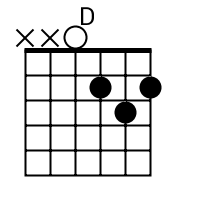
\includegraphics[width=3cm]{../Akordy/d.png}
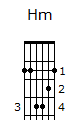
\includegraphics[width=3cm]{../Akordy/hm.png}
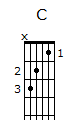
\includegraphics[width=3cm]{../Akordy/c.png}
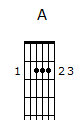
\includegraphics[width=3cm]{../Akordy/a.png}
\end{figure}
\newpage
\addcontentsline{toc}{section}{Cestou od hřbitova}\begin{song}{title=\centering Cestou od hřbitova \\\normalsize Znouzecnost  \vspace*{-0.3cm}}  %% sem se napíše jméno songu a autor
\moveright 4.2cm \vbox{      %Varianta č. 1  ---> Jeden sloupec zarovnaný na střed	

\sloka
	^{G{\color{white}aaa}}Cestou od hřbitova ^{D{\color{white}aaa}}potkal jsem tu madam,
	
	^{F}slzy se jí pod závojem ^{G{\color{white}aa}}derou do očí,
	
	ňáká mladá vdova -- ^{D}tak upřímnou soustrast
	
	^{F{\color{white}aaaa}}popřeju jí na začátek ^{G}a už se to točí.
	
\refren 
	Laj laj \dots \textbf{G, D, F, G, D, F, G}

	/: ^{G{\color{white}aa}}Svět, svět se ^{D{\color{white}aaaa}}zatočí a ^{F{\color{white}aa}}život jde ^{G}dál. :/ %Zatočí nebo točí? Já bych řekl, že zatočí, Ano, ztoci

\sloka
	Proč ty slzy, madam, vždyť žijem tak krátce,
	
	žal ve vaší tváři k vašemu já neladí.
	
	Nabízím Vám rámě -- služebník a rádce
	
	a kašlete na ty řeči, že se to nehodí.

\refren

\sloka
	Budu Vám číst z dlaní, co vás ještě čeká,
	
	něžně a s pietou vaše slzy osuším.
	
	Cestou od hřbitova jen chviličku váhá
	
	a ten pod tou hlínou už stejně nic netuší.

\refren

\sloka
	Balím holky na hřbitově přes duchovní útěchu,
	
	no a potom cestou domů skončí u mě v pelechu.
	
	Jsem dle řečí na pavlači amorální dobytek.
	
	A můj názor na celou věc: Oboustrannej užitek!

\refren


}
\setcounter{Slokočet}{0}
\end{song}


\newpage
\addcontentsline{toc}{section}{Černej pasažér}%\documentclass[../main.tex]{subfiles}

\begin{song}{title=\centering Černej Pasažér \\\normalsize Traband \vspace*{-0.3cm}}  %% sem se napíše jméno songu a autor
\moveright 1cm \vbox{      %Varianta č. 1  ---> Jeden sloupec zarovnaný na střed
\begin{minipage}[t]{0.48\textwidth}\setlength{\parindent}{0.25cm}  %Varianta č. 2 --> Dva sloupce
\setcounter{Slokočet}{0}
\sloka
Mám ^{Dmi}kufr plnej přebytečnejch ^{A}krámů 
                        
a mapu zabalenou do ^{Dmi}plátna 
                              
Můj vlak však jede na opačnou ^{A}stranu 
                               
a moje jízdenka je dávno ^{Dmi}neplatná 

\mezera
\textbf{F  Dmi F  Dmi }

\sloka
Někde ve vzpomínkách stojí dům 

Ještě vidím, jak se kouří z komína 

V tom domě prostřený stůl 

Tam já a moje rodina 

\sloka
Moje minulost se na mě šklebí 

a srdce bolí, když si vzpomenu 

že stromy, který měly dorůst k nebi 

teď leží vyvrácený z kořenů 

\mezera
\textbf{F  Dmi F  Dmi }

\refren
Jsem černej^{B} pasažér 

^{C}nemám ^{F}cíl ani směr 

Vezu se ^{B}načerno ^{C}životem a ^{F}nevím 
             
Jsem černej^{B} pasažér 

^{C}Nemám ^{F}cíl ani směr 

Vezu se ^{B}odnikud ^{C}nikam a ^{A7}nevím, kde skončím

\end{minipage}\begin{minipage}[t]{0.48\textwidth}\setlength{\parindent}{0.45cm}  % V případě varianty č.2 jde odsud text do pravé části
\vspace*{0.6cm}

\sloka
Mám to všechno na barevný fotce  

někdy z minulýho století 

Tu jedinou a pocit bezdomovce 

si nesu s sebou jako prokletí

\mezera
\textbf{F  Dmi F  Dmi }

\refren

\sloka
Mám kufr plnej přebytečnejch krámů 

a mapu zabalenou do plátna 

Můj vlak však jede na opačnou stranu 

a moje jízdenka je dávno neplatná

\refren

\end{minipage}   %Součást druhé varianty
}
\end{song}
\setcounter{Slokočet}{0}
\newpage
\addcontentsline{toc}{section}{Černobílý svět}%../main.tex]{subfiles}

\begin{song}{title=\centering Černobílý svět \\\normalsize Totální nasazení \vspace*{-0.3cm}}
%\vspace*{-1.2cm}
\moveright \stred \vbox{      %Varianta č. 1  ---> Jeden sloupec zarovnaný na střed
\setcounter{Slokočet}{0}
\sloka
^{Dmi}Jsme loutky ^{F}bez nití

^{B}já i všech ^{C{\color{white}\_\_\_}}patnáct druhů ^{Dmi}mých.

Bez smrti ^{F}bez žití

^{B{\color{white}\_\_\_\_}}bloumáme ^{C{\color{white}\_}}tupě po polích.

\refren
^{Dmi}Černá a ^{B{\color{white}\_}}bílá je,

^{C{\color{white}\_}}osm kroků tam a osm^{Dmi}sem,

frontová ^{B{\color{white}\_}}linie.

^{C}Na věky proti sobě ^{Dmi}jdem.

\sloka
^{Dmi}Stojí tu ^{F{\color{white}\_\_}}opodál

^{B}náš ^{{\color{white}\_\_\_}C}domnělý to ^{{\color{white}\_\_}Dmi}nepřítel.

I když jsem ^{F{\color{white}\_}}černý král

^{B{\color{white}\_\_}}nejsem svých ^{C\,\,\,\,}figur ^{{\color{white}\_}Dmi}velitel.

\sloka
Vždy první na tahu

jsem ten kdo bitvu rozpoutá,

ač nemá odvahu.

Bílý a nešťastný jsem král

\refren

\sloka
Přestal jsem počítat,

kolikrát jsem padnul a zas vstal,

kolikrát dostal mat,

útočil nebo utíkal

\sloka
Jsme jenom figury

ať král či pěšák beze jména

a hraní na vojáky je vaše lidská doména.

\refren

}
\end{song}
\setcounter{Slokočet}{0}
\newpage
\addcontentsline{toc}{section}{Danse macabre}\begin{song}{title=\centering Danse Macabre \\\normalsize Jaromír Nohavica \vspace*{-0.3cm}}  %% sem se napíše jméno songu a autor
\moveright 4cm \vbox{      %Varianta č. 1  ---> Jeden sloupec zarovnaný na střed	


\refren 
	^{Dmi B Dmi B Dmi B Dmi B Dmi F A Dmi B F C F A}{Naj, naj naj naj, naj naj naj\elipsa.\elipsa.\elipsa. \textcolor{white}{\hrulefill }} 
	%Geniální typografické řešení! % LIKE! To vypada elegantne. A.

\sloka
	^{Dmi}Šest milionů srdcí vyletělo ^{{\color{white}\_\_\_}B}komínem,

	^{Dmi}svoje malé lži si, lásko, dnes ^{{\color{white}\_\_\_\_}B}prominem,

	^{F{\color{white}\_\_\_\_}}budeme tančit s ^{A{\color{white}\_\_\_\_\_\_\_}}venkovany,

	na návsi ^{Dmi{\color{white}\_\_\_}}vesnice, budeme se ^{B{\color{white}\_\_}}smát, ^{F\,\,C}
	
	mám tě ^{F\,\,\,\,}rád. ^{A}

\refren

\sloka
	Láska je nenávist a nenávist je láska,
	
	jedeme na veselku, kočí bičem práská,
	
	v červené sametové halence

	podobáš se Evě i Marii,
	
	dneska mě zabijí.
	
\refren

\sloka
	Mě děti pochopily, hledí na mě úkosem,

	třetí oko je prázdný prostor nad nosem,
	
	Pánbůh se klidně opil levným balkánským likérem

	a teď vyspává,
	
	jinak to smysl nedává.


}
\setcounter{Slokočet}{0}
\end{song}



\newpage
\addcontentsline{toc}{section}{Dej mi víc své lásky}\begin{song}{title=\centering Dej mi víc své lásky \\\normalsize Olympic  \vspace*{-0.3cm}}  %% sem se napíše jméno songu a autor
\moveright \stred \vbox{      %Varianta č. 1  ---> Jeden sloupec zarovnaný na střed	

\sloka
	^{Emi{\color{white}\_\_}}Vymyslel jsem spoustu napadů, ^{G}aů,
   
	co ^{Emi{\color{white}\_\_}}podporujou hloupou ^{{\color{white}\_}D}náladu, ^{H7}aů,

	^{Emi}hodit klíče do kanálu, ^{A}sjet po zadku ^{Ami}holou skálu,

	v ^{Emi}noci chodit ^{H7\,\,\,\,}strašit do ^{{\color{white}\_}Emi}hradu, aů.

\sloka
	Dám si dvoje housle pod bradu, aů,

	v bílé plachtě chodím pozadu, aů,
	
	úplně melancholicky, s citem pro věc jako vždycky

	vyrábím tu hradní záhadu, aů.

\refren
	^{G}Má drahá, dej mi víc, ^{H7}má drahá, dej mi víc,

	^{Emi}má drahá, ^{C}dej mi víc své ^{G{\color{white}\_\_}}lásky, ^{D7}aů,

	^{G}já nechci skoro nic, ^{H7}já nechci skoro nic,

	^{Emi}já chci jen ^{C{\color{white}\_\_\_}}pohladit tvé ^{G{\color{white}\_\_}}vlásky, ^{H7}aů.

\sloka
	Nejlepší z těch divnejch nápadů, aů,
	
	mi dokonale zvednul náladu, aů,

	natrhám ti sedmikrásky, tebe celou s tvými vlásky

	zamknu si na sedm západů, aů.

\refren

\sloka = 3.


}
\setcounter{Slokočet}{0}
\end{song}



\newpage
\addcontentsline{toc}{section}{De N\^{i}mes}\begin{song}{title=\centering De N\^{i}mes \\\normalsize Radůza  \vspace*{-0.3cm}}  %% sem se napíše jméno songu a autor
\moveright 1.7cm \vbox{      %Varianta č. 1  ---> Jeden sloupec zarovnaný na střed	

\begin{minipage}[t]{0.48\textwidth}\setlength{\parindent}{0.45cm}  %Varianta č. 2 --> Dva sloupce

\textbf{Ami\,\,Dmi\,\,G\,\,Emi\,\,Ami}
       
\sloka 
	^{Ami{\color{white}\_}}Očima uhla ^{Dmi}jsem

	^{G}a nebylo to ^{{\color{white}\_\_}Ami}studem,

	peřina pohla ^{Dmi}se

	^{G}nějak už ^{{\color{white}\_}Ami}bude.

	\phantom{.}

	Lino je studený

	ponožky a pak triko
   	
	a kabát přes denim
	
	a nic a ticho

\ssloka{\textbf{R_{1}}:}
	Cette chanson n’a ^{Ami}jamais été chantée

	comme il ^{Dmi}faut, c’est ça.

	Mais si tu ^{G}veux, nous tous les ^{Emi}deux
  
	pouvons le ^{Ami}faire, comme ça.

	\phantom{.}

	La tranquillité, c’est ce qu’on cherche
	
	on dit: ,,Puisse-t-elle venir!''
	
	On dit que tout est dificile

	mais, qu’ est-ce que ça veut dire.

\ssloka{\textbf{R_{2}}:}
	Zouvám si pár těžkejch bot
	
	si ve vesmíru můj pevnej bod
	
	a sukně kasám, je blízko brod
	
	a pryč je, co kdo zbod.

\end{minipage}\begin{minipage}[t]{0.48\textwidth}\setlength{\parindent}{0.45cm}\vspace*{0.55cm}  % V případě varianty č.2 jde odsud text do pravé části

\sloka
	Jen hlesnu od dveří
	
	víš, nelhala jsem dosud

	a jestli nevěříš,
	
	zkus špičku nosu.

	Okna jsou zamlžený,

	nádobí škopek plnej,

	mám hrdlo stažený
	
	hajej a nynej.

\ssloka{\textbf{R_{1}}:}

\ssloka{\textbf{R_{2}}:}

\phantom{.}

2x 
\textbf{Ami\,\,Dmi\,\,G\,\,Emi\,\,Ami}
       
\ssloka{\textbf{R_{2}}:}

\sloka
	Očima uhla jsem
	
	a nebylo to studem
	
	poznal si po hlase,

	jak mi teď bude.
	
	Lino je studený

	pod kafem stůl se kejvá
	
	un souvenir de N\^{i}mes
	
	tak už to bejvá.

\ssloka{\textbf{R_{1}}:}

\ssloka{\textbf{R_{2}}:}



\end{minipage}
}
\vspace*{2cm}
\moveright 1.7cm \vbox{      %Varianta č. 1  ---> Jeden sloupec zarovnaný na střed	

% Výslovnostní poznámka:\\
\phantom{.}

\begin{minipage}[t]{0.48\textwidth}\setlength{\parindent}{0.45cm}  %Varianta č. 2 --> Dva sloupce
\textbf{R_1}: 

  [Set šanson nežame ete šanté 

  kom il fo se sa 

  me si ty v ni tu led

  puvon le fér, kom sa.]

\end{minipage}\begin{minipage}[t]{0.48\textwidth}\setlength{\parindent}{0.45cm}%\vspace*{0.55cm}  % V případě varianty č.2 jde odsud text do pravé části
\phantom{.}

[Le trankilité se s kon šerš

  on dy pui tel venir

  on dy k tu e dyfisil

  me kes ke sa v dire.]
\end{minipage}\\\\\\
% Texty překládat nebudeme. Věříme, že o významu jakékoliv písničky by člověk\\ měl přemýšlet především sám.
}
\setcounter{Slokočet}{0}
\end{song}
\newpage
\addcontentsline{toc}{section}{Dezolát}\begin{song}{title=\centering Dezolát\\\normalsize Vypsaná Fixa \vspace*{-0.3cm}}  %% sem se napíše jméno songu a autor
\moveright 2cm \vbox{      %Varianta č. 1  ---> Jeden sloupec zarovnaný na střed	
\begin{minipage}[t]{0.48\textwidth}\setlength{\parindent}{0.45cm}  %Varianta č. 2 --> Dva sloupce

\sloka
	^{Emi}Ty jsi pěkný ^{\,\,C}dezolát,
	
	^{D{\color{white}\_}}řekla ,,Halí ^{A}Belí''
	
	a byla to pohoda,
	
	třeba se to povede, 
	
	vytáhnem tvý múzy 
	
	a hodíme je za tebe 
	
	a kdo ty múzy zachytí, 

	ten bude mít záruku 
	
	opravdový kvality.
	
	Ty jsi pěkný dezolát.
	
	Tohle řekla ona, 
	
	musíme tě sledovat.
	
\refren
	^{C}A celý ^{Emi}prostor 
	
	je sledovaný
	
	^{C}příjemnými lidmi, kteří olizují 
	
	^{C}šťávu ^{Emi}tekoucí 
	
	z konečků ^{D}prstů.
	
\sloka
	Ty jsi pěkný dezolát.
	
	Ve sprchovým koutě 
	
	teče voda ledová.
	
	Třeba se to povede,
	
	opláchnu svý múzy 
	
	a vypustím je pod sebe. 
	
	Kdo ty múzy zachytí, 
	
	ten bude mít záruku 
	
	opravdový kvality. 
	
	Ty jsi pěkný dezolát. 
	
	Tohle řekla ona.
	
\refren
	
      \end{minipage}\begin{minipage}[t]{0.48\textwidth}\setlength{\parindent}{0.45cm}%\vspace*{0.55cm}  % V případě varianty č.2 jde odsud text do pravé části

\refren
	^{Emi{\color{white}\_\_}}Pustíme si ^{C{\color{white}\_}}starý gramofon, 
	
	^{D{\color{white}\_\_\_\_\_\_\_}}budeme mít ^{A{\color{white}\_}}světy, 
	
	který nás zajímají.
	
	Vinylový bůh je šampion,
	
	proležíme v posteli 
	
	celou neděli.
	
	Pustíme si starý gramofón,
	
	budeme mít světy,
	
	který nás zajímají.
	
	Viny loví bůh, je šampion,
	
	venku ten náš svět 
	
	sledují kamery.
	
	\phantom{h}
	
	A hudba hraje dál\dots
	
	\phantom{h}	
	
	Pustíme si starý gramofon,
	
	budeme mít světy, 
	
	který nás zajímají.
	
	Vinylový bůh je šampion,
	
	venku ten náš svět 
	
	sledují kamery.
	
	\phantom{j}
	
	^{Emi}Jsem z ^{C}toho celej ^{A}žhavej.
	
	
\end{minipage}
}
\setcounter{Slokočet}{0}
\end{song}



\newpage
\addcontentsline{toc}{section}{Do Ameriky}\documentclass[../main.tex]{subfiles}

\chapter*{Do Ameriky}

\noindent\hspace{0.15\linewidth}
\begin{minipage}{0.7\linewidth}
\begin{song}{title=Do Ameriky}

\begin{verse}[numbered]
	^{D}Do Ameriky jezděj Parníky,\\
	když tam přijdeš, zdá se ti to ^{A7}všecko veliký,\\
	^{\phantom{S}}je to fakticky tuze praktický  \\
	když tam přijdeš, umět anglic^{D}ky. \\
\end{verse}

\begin{verse*}
	Refrain:
	^{D}Dobrou noc - good night, ^{A7}výborně - all right,\\
	Konrád White, už je off^{D}side (housemister - Dally sister!) \\
	^{D}Dneska je today, ^{A7}dobrý den - good day,\\
	já jsem byl taky chu^{D}dej. \\ 
	^{G}His Master's Voice, Yankee Doo^{G}dle,\\ \\
	^{En7}máš apetit? (mám) ^{A7}vem si štrůdl! (do pusy)\\
	^{D}Sto kilo je cent, ^{A7}patent je patent,\\
	husa v troubě happy^{D}end.
\end{verse*}

\begin{verse}[numbered]
	Co Buffalo Bill vrazil do kobyl,\\
	za to by si bejval byl koupil automobil,\\
	cowboy na koni už se nehoní,\\
	přestože mu Fordka nevoní.\\
\end{verse}

\begin{verse*}
	Refrain
\end{verse*}

\begin{verse}[numbered]
	Mám na západě chajdu v Nevadě,\\
	zlatou žílu v Arizoně, doly v Kanadě,\\
	babička na mě šetří v Panamě\\
	a já si tu žiju náramě!\\
\end{verse}



\end{song}

\end{minipage}\newpage
\addcontentsline{toc}{section}{Do dne a do roka}%\documentclass[../main.tex]{subfiles}


\begin{song}{title=\centering Do dne a do roka \\ \normalsize Jaromír Nohavica \vspace*{-0.3cm}}  %% sem se napíše jméno songu a autor
\moveright 2cm \vbox{      %Varianta č. 1  ---> Jeden sloupec zarovnaný na střed
\begin{minipage}[t]{0.48\textwidth}\setlength{\parindent}{0.45cm}  %Varianta č. 2 --> Dva sloupce
\setcounter{Slokočet}{0}
%\centering
\sloka
^{Hmi C#7 F#m } 

Byla ^{Hmi}hluboká noc^{C#7} 

Venku ^{F#m}cizí pes vil 

A ja ^{Hmi}u okna stál^{C#7}  

A ^{F#m}pil 

\sloka
Zřel jsem ^{Hmi}jen jeho stín^{C#7}

Měl ^{F#m}rozplizlý tvar 

A ^{Hmi}vypadal jak^{C#7} 

Lomi^{F#m}kar 

\refren
Do dne a ^{Hmi}do roka, za zvuku ^{C#7}baroka, se rodí ^{F#m}rokoko 

Do noci ^{Hmi}hledíme, a vlastně ^{C#7}nevíme, 

zda je to ^{F#m}opravdu anebo jenom tak, naoko 

Do dne a ^{Hmi}do roka, za zvuku ^{C#7}rokoka, se rodí ^{F#m}secese 

Do noci ^{Hmi}hledíme, všichni tam ^{C#7}musíme, ale ^{F#m}nechce se 

\sloka
Chtěl jsem okřiknout jej, 

myslím psa v oné tmě, 

ale neměl jsem slov, jimiž to lze.

Vzal jsem do ruky kolt, 

jenž v mé komodě byl 

a na černý stín jsem namířil. 
\end{minipage}\begin{minipage}[t]{0.48\textwidth}\setlength{\parindent}{0.45cm}  % V případě varianty č.2 jde odsud text do pravé části
\sloka
Ruka chvěla se mi, 

neboť z krbu šel mráz, 

pak se na vteřinu zastavil čas. 

Tmě se zježila srst, 

já ucítil strach, 

kdo má na spoušti prst je vrah.

\refren
%\newpage
\sloka
Výstřel protrhl tmu, 

jako rybářům síť, 

jako sudičce řeč a niť. 

Té noci špatně jsem spal 

v záři voskových svic,

ráno tam, co byl plot, nebylo nic. 

\refren
\end{minipage}
}
\end{song}

\newpage
\addcontentsline{toc}{section}{Dokud se zpívá}\begin{song}{title=\centering Dokud se zpívá \\\normalsize Jaromír Nohavica  \vspace*{-0.3cm}}  %% sem se napíše jméno songu a autor
\moveright 3.8cm \vbox{      %Varianta č. 1  ---> Jeden sloupec zarovnaný na střed	

\sloka 
	^{C}Z Těšína ^{Emi\,\,\,\,\,}vyjíždí ^{Dmi7}vlaky co ^{F{\color{white}aaaaaa}C}čtvrthodinu, ^{Emi\,Dmi7\,G}

	včera jsem nespal a ani dnes nespočinu,

	^{F}svatý ^{G}Medard, můj ^{C}patron, ťuká ^{Ami}si na ^{{\color{white}aa}G}čelo,

	ale ^{F}dokud se ^{G}zpívá, ^{F}ještě se ^{G{\color{white}aaaa}C}neumřelo. ^{Emi\,Dmi7\,G}

\sloka
	Ve stánku koupím si housku a slané tyčky,
	
	srdce mám pro lásku a hlavu pro písničky,
	
	ze školy dobře vím, co by se dělat mělo,
	
	ale dokud se zpívá, ještě se neumřelo.

\sloka
	Do alba jízdenek lepím si další jednu,
   
	vyjel jsem před chvílí, konec je v nedohlednu,
	
	za oknem míhá se život jak leporelo,
	
	ale dokud se zpívá, ještě se neumřelo.

\sloka
	Stokrát jsem prohloupil a stokrát platil draze,
	
	houpe to, houpe to na housenkové dráze,
	
	i kdyby supi se slítali na mé tělo,
	
	tak dokud se zpívá, ještě se neumřelo.

\sloka
	Z Těšína vyjíždí vlaky až na kraj světa,
	
	zvedl jsem telefon a ptám se: \uv{Lidi, jste tam?}
	
	A z veliké dálky do uší mi zaznělo,
	
	/: že dokud se zpívá, ještě se neumřelo. :/


}
\setcounter{Slokočet}{0}
\end{song}
\newpage
\addcontentsline{toc}{section}{Franky Dlouhán}\begin{song}{title=\centering Franky Dlouhán \\\normalsize Brontosauři  \vspace*{-0.3cm}}  %% sem se napíše jméno songu a autor
\moveright \stred \vbox{      %Varianta č. 1  ---> Jeden sloupec zarovnaný na střed	

\sloka 
	^{C}Kolik je smutného,
	
	když ^{F} mraky černé ^{C}jdou

	lidem nad ^{G}hlavou ^{F}smutnou dálavo^{C}u.
	
	Já slyšel příběh, který velkou pravdu měl,
	
	za čas odletěl, každý zapomněl.

\refren
	^{C}Měl kapsu ^{G}prázdnou Franky Dlouhán,

	po státech ^{F}toulal se jen ^{C}sám, a že

	byl ^{F}veselej, tak ^{C}každej měl ho ^{G7}rád.

	Tam ruce k ^{F}dílu mlčky přiloží a ^{C}zase

	jede ^{Ami}dál. A ^{F}každej kdo s ním

	^{G}chvilku byl, tak ^{F}dlouho ^{G7}se pak ^{C}smál.
	
\sloka	
	Tam, kde byl pláč, tam Franky hezkou píseň měl,
	
	slzy neměl rád, chtěl se jenom smát.
	
	A když pak večer ranče tiše usínaj,
	
	Frankův zpěv jde dál nocí s písní dál.\elipsa\dots
	
\sloka
	Tak Frankyho vám jednou našli, přestal žít,
	
	jeho srdce spí, tiše smutně spí.
	
	Bůh ví jak, za co tenhle smíšek konec měl,
	
	farář píseň pěl, umíraček zněl.\elipsa\dots

}
\setcounter{Slokočet}{0}
\end{song}


\begin{figure}[h]
\centering
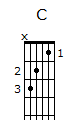
\includegraphics[width=3cm]{../Akordy/c.png}
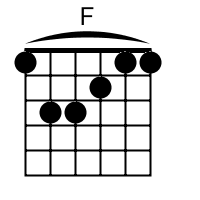
\includegraphics[width=3cm]{../Akordy/f.png}
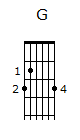
\includegraphics[width=3cm]{../Akordy/g.png}
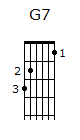
\includegraphics[width=3cm]{../Akordy/g7.png}
\end{figure}
	\newpage 
\addcontentsline{toc}{section}{God\ap s Gonna Cut You Down}\documentclass[../main.tex]{subfiles}

\chapter{God's gonna cut you down}

\noindent\hspace{0.15\linewidth}\begin{minipage}{0.7\linewidth}
\begin{song}{title=Johnny Cash - Gods gonna cut you down}
\begin{verse}[numbered]
You^{Am} can run on for a long time, \\
Run^{Am} on for a long time, \\
Run^{Am} on for a long time, \\
Sooner, or later^{Dm}, God'll cut you down^{Am}. \\
Sooner, or later^{Dm}, God'll cut you down^{Am}. \\
\end{verse}
\begin{verse}[numbered]
Go and tell^{Am} that long tongue liar, \\
Go and tell^{Am} that midnight rider, \\
Tell the rambler^{Am}, the gambler, the back biter, \\
Tell^{C} 'em that God's^{Em} gonna cut^{Am} 'em down. \\
Tell^{C} 'em that God's^{Em} gonna cut^{Am} 'em down. \\
\end{verse}
\begin{verse}[numbered]
Well my^{Am} goodness gracious, let me tell you the news. \\
My heads^{Am} been wet with the midnight dew. \\
I've^{Am} been down on bended knee, \\
talkin^{Am} to the man from Galiee. \\
He spoke^{Am} to me in a voice so sweet, \\
I thought^{Am} I heard the shuffle of angels feet.  \\
He called^{Am} my name and my heart stood still,  \\
When He^{Am} said^{Mute} \uv{John go do my will}  \\
\end{verse}
\begin{verse}[numbered]
Go and tell^{Am} that long tongue liar, \\
Go and tell^{Am} that midnight rider, \\
Tell the rambiler^{Am}, the gambler, the back biter, \\
Tell^{C} 'em that God's^{Em} gonna cut 'em down^{Am}. \\
Tell^{C} 'em that God's^{Em} gonna cut 'em down^{Am}. \\
\end{verse}
\end{song}
\end{minipage}

\newpage
\vspace*{4.5cm}
\noindent\hspace{0.15\linewidth}\begin{minipage}{0.7\linewidth}
\begin{song}{title=Johnny Cash - Gods gonna cut you down}
\begin{verse}
\item[5.]You can run^{Am} on for a long time, \\
Run^{Am} on for a long time, \\
Run^{Am} on for a long time, \\
Sooner^{C}, or later,^{Em} God'll cut^{Am} you down. \\
Sooner^{C}, or later,^{Em} God'll cut^{Am} you down. \\
You may throw^{Am} your rock, hide your hand, \\
Workin^{Am} in the dark against your fellow man. \\
But as^{Am} sure as God made black and white, \\
What's done^{Am} in the dark, will be brought to the light. \\
\end{verse}
\begin{verse}
\item[6.]You can run^{Am} on for a long time, \\
Run^{Am} on for a long time, \\
Run^{Am} on for a long time, \\
Sooner^{C}, or later,^{Em} God'll cut^{Am} you down. \\
Sooner^{C}, or later,^{Em} God'll cut^{Am} you down. \\
\end{verse}
\begin{verse}
\item[7.]Go and tell^{Am} that long tongue liar, \\
Go and tell^{Am} that midnight rider, \\
Tell the rambler^{Am}, the gambler, the back biter, \\
Tell^{C} 'em that God's^{Em} gonna cut^{Am} 'em down. \\
Tell^{C} 'em that God's^{Em} gonna cut^{Am} 'em down^{Am}. \\
Tell^{C} 'em that God's^{Em} gonna cut^{Am} 'em down^{Am}. 
\end{verse}
\end{song}
\end{minipage}

\newpage
\addcontentsline{toc}{section}{Hallelujah}\begin{song}{title=\centering Hallelujah \\\normalsize Leonard Cohen / Jeff Buckley \vspace*{-0.3cm}}  %% sem se napíše jméno songu a autor

\fontsize{11pt}{12pt}\selectfont

\moveright 1cm \vbox{      %Varianta č. 1  ---> Jeden sloupec zarovnaný na střed
\begin{minipage}[t]{0.48\textwidth}\setlength{\parindent}{0.25cm}  %Varianta č. 2 --> Dva sloupce

\sloka
	I ^{C}heard there was a ^{Am}secret chord  
	
	That ^{C}David played and it ^{Am}pleased the lord  
	
	But ^{F}you don't really ^{G}care for music, ^{C}do you?^{G}  
	
	Well ^{C}it goes like this the ^{F}fourth, the ^{G}fifth  
	
	The ^{Am}minor fall and the ^{F}major lift  
	
	The ^{G}baffled king ^{E7}composing halle^{Am}lujah  
	

\refren
^{F}Hallelujah, ^{Am}hallelujah, ^{F}hallelujah,

 ^{C}halleluuu - u - ^{G}uuu - u - ^{C}jah \dots 

\sloka
	Your faith was strong, but you needed proof,  
	
	you saw her bathing on the roof,  
	
	her beauty and the moonlight overthrew you.  
	
	She tied you to a kitchen chair,  
	
	she broke your throne, and she cut your hair,  
	
	and from your lips she drew the Hallelujah!  


\refren


\sloka
	You say I took the name in vain,  
	
	I don't even know the name,  
	
	but if I did, well really, what's it to you?  
	
	There's a blaze of light in every word,  

	it doesn't matter which you heard,  
	
	the holy or the broken Hallelujah!  
	

\refren

\sloka
	Baby, I've been here before,  
	
	I know this room, I've walked this floor,  
	
	I used to live alone before I knew you.  
	
	I've seen your flag on the marble arch,  
	
	but love is not a victory march,  
	
	it's a cold and it's a broken Hallelujah!  


\end{minipage}\begin{minipage}[t]{0.48\textwidth}\setlength{\parindent}{0.45cm}  % V případě varianty č.2 jde odsud text do pravé části
\vspace*{0.6cm}
\refren

\sloka
	There was a time you let me know,   
	
	what's really going on below,   
	
	but now you never show it to me, do you?   
	
	But I remember, when I moved in you,   
	
	and the holy dove was moving too,   
	
	and every breath we drew was Hallelujah!   
	
\refren

\sloka
	Maybe there's a God above,   
	
	but all I've ever learned from love   
	
	was how to shoot at someone who outdrew you.   
	
	But it's not a cry that you hear at night,   
	
	it's not somebody who's seen the light,   
	
	it's a cold and it's a broken Hallelujah!   
	
\sloka
	I did my best, it wasn't much,   
	
	I couldn't feel, so I tried to touch,   
	
	I've told the truth, I didn't come to fool you.   
	
	And even though it all went wrong,   
	
	I'll stand before the Lord of Song   
	
	with nothing on my tongue but Hallelujah!   
	

\refren

\end{minipage}   %Součást druhé varianty
}
\setcounter{Slokočet}{0}
\end{song}

\newpage  % Pouze jednostranná verze
% \addcontentsline{toc}{section}{Hero of War}\begin{song}{title=\centering Hero of War \\\normalsize Rise against  \vspace*{-0.3cm}}  %% sem se napíše jméno songu a autor
\moveright \stred \vbox{      %Varianta č. 1  ---> Jeden sloupec zarovnaný na střed	

\sloka 
	He said, \uv{ ^{Em}Son,

	Have you seen the ^{H}world?

	Well, what would you ^{A}say
                   
	If I said that you ^{Emi}could?
               
	Just carry this ^{A}gun 
                   
	and you’ll even get ^{Emi}paid.}
                            
	I said, \uv{That sounds pretty ^{H}good.}
              
	Black leather ^{Emi}boots
              
	Spit-shined so ^{H}bright
                
	They cut off my ^{A}hair 
             
	but it looked ^{Emi}alright
                 
	We marched and we ^{A}sang
              
	We all became ^{Emi}friends
                     
	As we learned how to ^{H}fight


\refren
	A hero of ^{F\# mi}war

	Yeah that’s what I’ll ^{A}be
               
	And when I come ^{Emi}home
                        
	They’ll be damn proud of ^{H}me
               
	I’ll carry this ^{F\# mi}flag
                 
	To the grave if I ^{A}must
                        
	Because it’s flag that I ^{Emi}love
                  
	And a flag that I ^{H}trust


\sloka
	I kicked in the ^{Emi}door
             
	I yelled my ^{H}commands
                   
	The children, they ^{A}cried
              
	But I got my ^{Emi}man
            
	We took him ^{A}away
                
	A bag over his ^{Emi}face
                       
	From his family and his ^{H}friends

	They took off his ^{Emi}clothes
                 
	They pissed in ^{H}his hands
                
	I told them to ^{A}stop
              
	But then I ^{Emi}joined in
                 
	We beat him with ^{A}guns
                  
	And batons not just ^{Emi}once
               
	But again and ^{H}again


\refren


\sloka
	She ^{Emi}walked 
                    
	through bullets and ^{H}haze
                
	I asked her to ^{A}stop
               
	I begged her to ^{Emi}stay
               
	But she pressed ^{A}on
                
	So I lifted my ^{Emi}gun
             
	And I fired ^{H}away
    
	The ^{Emi}shells 
                    
	jumped through the ^{H}smoke
             
	And into the ^{A}sand
                        
	That the blood now had ^{Emi}soaked
        
	She ^{A}collapsed 
                   
	with a flag in her ^{Emi}hand
                
	A flag white as ^{H}snow


\sloka
	A hero of ^{F\# mi}war
                 
	Is that what the ^{A}see
                
	Just medals and ^{E}scars
                
	So damn proud of ^{H}me
                        
	And I brought home that ^{F\# mi}flag
               
	Now it gathers ^{A}dust
                        
	But it’s a flag that I ^{E}love
                       
	It’s the only flag I ^{H}trust


\refren
He said, \uv{ ^{Emi}Son, 
                   
have you seen the ^{H}world? 
                    
Well what would you ^{A}say, 
                   
if I said that you ^{Emi}could?}







\setcounter{Slokočet}{0}
\end{song}


\newpage % Neni ocheckovano
\addcontentsline{toc}{section}{Hey Ho}\begin{song}{title=\predtitle\centering Hey Ho Nobody's Home \vspace*{-0.3cm}}  %% sem se napíše jméno songu a autor
\begin{centerjustified}
\nejnejvetsi
	
\sloka
^{Ami}Hey ^{Emi}ho, ^{Ami}nobody's ^{Emi}home, 

^{Ami}Meat nor ^{Emi}drink nor ^{Ami}money have I ^{Emi}none. Yet 

^{Ami}Every ^{Emi}time I ^{Ami}will be ^{Emi}happy. 

/: ^{Ami}Zum gali ^{Emi}gali gali, ^{Ami}zum gali ^{Emi}gali. :/

\end{centerjustified}
\setcounter{Slokočet}{0}
\end{song}

\begin{figure}[h]
\predtitle\centering
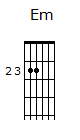
\includegraphics[width=3cm]{../Akordy/em.png}
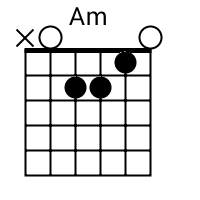
\includegraphics[width=3cm]{../Akordy/am.png}
\end{figure}
\newpage
\addcontentsline{toc}{section}{Hlídač krav}%\documentclass[../main.tex]{subfiles}

\begin{song}{title=\centering Hlídač krav \\\normalsize Jaromír Nohavica \vspace*{-0.3cm}}  %% sem se napíše jméno songu a autor
\moveright \stred \vbox{      %Varianta č. 1  ---> Jeden sloupec zarovnaný na střed

\sloka
^{C{\color{white}\_\_}}Když jsem byl malý, říkali mi naši,

dobře se uč a jez vtipnou kaši,

až ^{F{\color{white}\_\_\_\_}}jednou vyrosteš, ^{G7{\color{white}\_\_}}budeš doktorem ^{C{\color{white}\_\_}}práv. 

Takovej doktor si sedí pěkně v suchu,

bere velký peníze a škrábe se v uchu,

ja jim na to řek!: \uv{chci být hlídačem krav}.

\refren
^{G7}Já chci: ^{C}Mít čapku s bambulí nahoře,

jíst kaštany a mýt se v lavoře, 

^{F}od rána po celý ^{G7}den zpívat si ^{C}jen. 

^{G7{\color{white}\_\_}}Zpívat si: ^{C\,\,F\,\,G7\,\,C\,\,}pam\,pam\,pam\elipsa.\elipsa.\elipsa.

\sloka
K vánocům mi kupovali hromadu knih,

co jsem ale vědět chtěl, to nevyčet' jsem z nich,

nikde jsem se nedověděl, jak se hlídají krávy.

Ptal jsem se starších a ptal jsem se všech,

každý na mě koukal jako na pytel blech,

každý se mě opatrně tázal na moje zdraví.

\refren

\sloka
Dnes už jsem starší, vím co vím,

mnohé věci nemůžu a mnohé smím,

a když je mi velmi smutno, lehnu si do mokré trávy.

S nohama křížem, rukama za hlavou,

koukám nahoru, na oblohu modravou,

kde se mezi mraky honí moje strakaté krávy.

\refren

\sloka
^{D\, G\, A7\, D\, E\, A\, H7\, E}Pam\,pam\,pam\elipsa.\elipsa.\elipsa.  

}
\setcounter{Slokočet}{0}
\end{song}
\newpage
\addcontentsline{toc}{section}{Hotel Hillary}\begin{song}{title=\centering Hotel Hillary \\\normalsize Poutníci \vspace*{-0.3cm}}  %% sem se napíše jméno songu a autor
\moveright 3.8cm \vbox{      %Varianta č. 1  ---> Jeden sloupec zarovnaný na střed	

\sloka 
	Tvař se ^{Ami}trochu nostalgicky, už tě nikdy nepotkám,

	^{F}máš to jistý ^{G}provždycky, nastav ^{Ami}uši vzpomínkám,

	jak tě znám, i v tuto chvíli měl bys řeči peprný,
    
	jak ^{F{\color{white}\_\_\_\_}}tenkrát, když nám ^{G{\color{white}\_\_\_}}tvrdili, že je ^{Ami}vítr stříbrný.


\refren
	A ^{F{\color{white}\_\_}}tváře měli kožený, my jim zdrhli z průvodu,

	^{Dmi{\color{white}\_\_}}zahodili lampióny a ^{D{\color{white}\_\_\_}}našli hospodu,

	ale ^{F{\color{white}\_\_}}taky Jacquese Brela a s ním smutek z cizích vin

	a ^{Dmi{\color{white}\_\_\_\_\_\_}}žádostivost těla a pak ^{D{\color{white}\_\_\_}}radost z volovin, a ta nám ^{Ami{\color{white}\_\_}}zbejvá.

\sloka
	Po večerech pro diváky dělali jsme kašpary,
	
	pak na zemi dva spacáky -- náš Hotel Hillary,
	
	slavný sliby jsme už znali i to, jak se neplní,
	
	a cenzoři nám kázali vo správným umění.

\refren

\sloka	
	A tak válčím s nostalgií, bují ve mně jako mech,
	
	a pořád všechno slibují starý hesla na domech,
	
	ty jsi splatil všechny dluhy i za Hotel Hillary
	
	a já vyhážu ty černý stuhy funebrákům navzdory.

\refren
	Vždyť mají tváře kožený, my jim zdrhnem z průvodu,
	
	zahodíme lampióny a najdem hospodu,
	
	a tam tvýho Jacquese Brela a s ním smutek z cizích vin
	
	a žádostivost těla a pak radost z volovin, /: a ta nám zbejvá. :/



}
\setcounter{Slokočet}{0}
\end{song}
\newpage
\addcontentsline{toc}{section}{House Of The Rising Sun}\begin{song}{title=\predtitle\centering House Of The Rising Sun \\\large \vspace*{-0.3cm}}  %% sem se napíše jméno songu a autor
\begin{centerjustified}
\nejvetsi

\sloka 
	^{Ami\,}There is a ^{C{\color{white}\_\_}}house in ^{D{\color{white}\_}}New ^{F}Orleans

	They ^{Ami}call the ^{C{\color{white}\_\_}}Rising ^{E}Sun

	And it's ^{Ami}been a ^{C}ruin of ^{D}many a poor ^{F}boy

	And ^{Ami}God I ^{E}know I'm ^{Ami}one. ^{C\,D\,F\,Ami\,E\,Ami\,E}

\sloka
	My mother was a tailor
	
	Sewed my new blue jeans,
	
	My father was a gamblin' man
   	
   	Down in New Orleans.

\sloka
	Now the only thing a gambler needs

	Is suitcase and trunk

	And the only time he's satisfied

	Is when he's on, a drunk.

\sloka
	Oh mother tell your children

	Not to do what I have done

	Spend your lives in sin and misery

	In the House of the Rising Sun.

\sloka
	Well, I've got one foot on the platform

	The other foot on the train

	I'm going back to New Orleans

	To wear that ball and chain.

\sloka = 1.


\end{centerjustified}
\setcounter{Slokočet}{0}
\end{song}

\begin{figure}[h]
\predtitle\centering
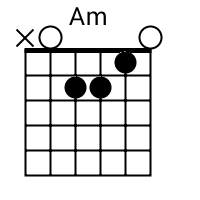
\includegraphics[width=3cm]{../Akordy/am.png}
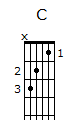
\includegraphics[width=3cm]{../Akordy/c.png}
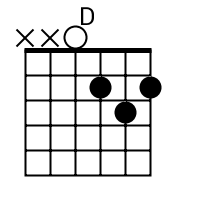
\includegraphics[width=3cm]{../Akordy/d.png}
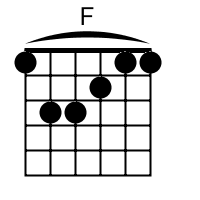
\includegraphics[width=3cm]{../Akordy/f.png}
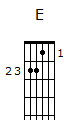
\includegraphics[width=3cm]{../Akordy/e.png}
\end{figure}
\newpage
% \addcontentsline{toc}{section}{Hruška}\begin{song}{title=\predtitle\centering Hruška \\\large Čechomor  \vspace*{-0.3cm}}  %% sem se napíše jméno songu a autor
\begin{centerjustified}
\nejnejvetsi

\sloka 
  ^{{\color{white}\_}D}Stojí hruška v  ^{{\color{white}\_}A}širém poli 
  
   ^{D{\color{white}\_\_}}vršek se ^{G}jí ^{{\color{white}\_\_}A}zelená.	
  
  /: Pod ^{D}ní se ^{G\,\,}pase ^{A}kůň ^{{\color{white}\_}Hmi}vraný, 
  
  ^{\,\,\,\,D}pase ho ^{A}má ^{\,\,\,\,D}milá. :/ 

\sloka
  Proč má milá dnes pasete 
  
  z večera do rána. 

  /: Kam můj milý pojedete, 

  já pojedu s váma. :/ 


\sloka
  O já pojedu daleko 

  přes vody hluboké. 
   
  /: Kéž bych byl nikdy nepoznal 

  panny černooké. :/


\end{centerjustified}
\setcounter{Slokočet}{0}
\end{song}
\newpage %Neni ocheckovano
\addcontentsline{toc}{section}{Hurt}\begin{song}{title=\centering Hurt \\\normalsize Johnny Cash \vspace*{-0.3cm}}  %% sem se napíše jméno songu a autor
\moveright 4.2cm \vbox{      %Varianta č. 1  ---> Jeden sloupec zarovnaný na střed	

\sloka 
	I ^{C}hurt ^{D2}myself ^{Ami}today to ^{C}see if ^{D2}I still ^{Ami}feel,

	^{\phantom{.}}I focus on the pain, the only thing that's real.
   	
   	^{\phantom{.}}The needle tears a hole, the old familiar sting,

	try to ^{C}kill it ^{D2}all ^{Ami}away, but ^{C}I ^{D2}remember ^{G}everything.


\refren
	^{Ami}What have I ^{\,\,\,\,Fmaj7}become, ^{C}my sweetest ^{G{\color{white}\_\_}}friend?
	
	^{\phantom{.}}Everyone I know goes away in the end.

	And ^{Ami}you could have it ^{Fmaj7}all, ^{G}my empire of dirt,
	
	^{\phantom{.}}I will let you down, I will make you hurt.

\sloka   
	 I wear this crown of thorns upon my liar's chair,
   	
   	full of broken thoughts I cannot repair.
   	
   	Beneath the stains of time the feeling disappears,
   	
   	you are someone else, I am still right here.


\refren\\
   
	^{Ami}If I could start ^{Fmaj7}again, a ^{G\,\,\,\,\,\,\,}million miles away,

	^{Ami}I would keep ^{\,\,\,\,Fmaj7}myself, ^{G}I would find a ^{Ami}way.
	
}
\setcounter{Slokočet}{0}
\end{song}

\newpage
\addcontentsline{toc}{section}{Chci ti říct}\begin{song}{title=\predtitle\centering Chci ti říct \\\large Mig 21  \vspace*{-0.3cm}}  %% sem se napíše jméno songu a autor
\begin{centerjustified}


\predehra
4$\times $\textbf{Gmi C2}

\sloka
	^{Gmi}Chladná ^{C2}rána jsou ^{Gmi}tomu, kdo ^{C2}strádá,

	^{Gmi\,\,}láskou ^{C2\z }bolestnou ^{Gmi\z C2}neopětovanou.

	Pokud ^{Gmi}víš, jak ^{C2}rád tě mám, ^{Gmi}a ty mě máš ^{C2}ráda.

	^{Gmi}Chuť a ^{C2}vůni tvou ^{Gmi}nejde ^{C2\z }zapomenout.

\sloka
	Chystá ^{Dmi}se prej konec ^{C2}světa, ^{Gmi}tramtadá

	a ^{Dmi}mě jen jedna ^{C2}věta ^{\z B2}napadá. (\dots\,tak pojď s tim ven!)

\refren
	^{F}Chci ti říct, že mám tě ^{C2}rád, že ^{Gmi}miluju tě jako blázen,

	^{F}chci si nechat ^{C2\z }tetovat jen ^{Gmi}jméno tvé, chci vypít bazén

	^{F}vody, kterou ^{C2\z }plavala jsi, ^{Gmi\z }zasadit si tvoje vlasy,

	^{F\z }rozfoukat je ^{C2}do ulic ^{Gmi}chci ti říct, že rád tě mám ^{B7}víc.

\sloka
	Dýcháš na mou tvář, já na tvou dýchám.

	Chvěješ se myšlenkou, že se rozední.

	Děláš, jako že nespěcháš, já že nepospíchám.

	Nechce se z objetí, když je poslední.

\sloka  = 2.

\refren


\sloka
	/: ^{B7}Mít tak promyšlenej plán, předem fakt moc se omlouvám, 

	ale ode dneška od půl jedný musíme bejt zodpovědný. :/

	^{B7}Mít tak promyšlenej plán, ale nemám ho, nemám ho, nemám\elipsa.\elipsa.\elipsa.\,a tak:

\refren


\end{centerjustified}
\setcounter{Slokočet}{0}
\end{song}
\newpage
\addcontentsline{toc}{section}{Je jaká je}%\documentclass[../main.tex]{subfiles}


\begin{song}{title=\centering Je jaká je \\\normalsize Karel Gott  \vspace*{-0.3cm}}  %% sem se napíše jméno songu a autor
\moveright 4cm \vbox{      %Varianta č. 1  ---> Jeden sloupec zarovnaný na střed

\sloka
^{D}Je jaká ^{F#mi}je, ^{G}tak mi ^{A}náhle padla ^{D}do  ^{F#mi}klína, 

^{G}ani ^{A}černá ^{D}ani ^{F#mi}blondýna, ^{G}někdy ^{A}tak a ^{D}jindy ^{Hmi}taková,

^{G}vždycky ^{A}hádam jak ^{D}se ^{Hmi G}zachová, ^{A}zřejmě ^{D}nikdy ^{Hmi}jak ^{G A}chci já

\sloka
Je jaká je, trochu dítě, trochu mondéna, 

nemám právě paměť na jména, tak jí říkám lásko má. 

Nejsi skvost a nejsi zlá, jsi jen jiná než chci já. 

\sloka
Je jaká je, že se změní čekat nedá se, 

snad jí záleží jen na kráse, tak, že člověk málem nedutá, 

jak je štíhlá, jak je klenutá, jenže jinak, než chci já. 

\sloka
Je jaká je, až jí zitra spatříš u pláže, 

vzkaž jí, ať se na mě neváže, ať si pro mě vrásky neděla, 

ať je jaká je a veselá, i když jiná než chci já. 

}
\setcounter{Slokočet}{0}
\end{song}

\newpage
\addcontentsline{toc}{section}{Ještě jedno kafe}\begin{song}{title=\predtitle\centering Ještě jedno kafe  \\\large Druhá Tráva a Robert Křesťan  \vspace*{-0.3cm}}  %% sem se napíše jméno songu a autor
\begin{centerjustified}
\nejnejvetsi

\sloka 
	Máš ^*{Emi}sladk ej dech a oči, kterým ^*{D}pa tří svatozář

	a ^*{C}vl asy máš jak hedvábí, když je ^*{H7}vho díš na polštář,

	ale ^{Emi}já se o tvou lásku ani ^*{D}vd ěčnost neprosím,

	ty ^*{C}dě kuješ jen hvězdám a jseš ^*{H7}věr ná jenom jim.

\refren
	^*{C}Je ště jedno kafe bych si ^{H7}dal,

	^*{C}je ště jedno kafe, ^{{\color{white}\_\_\_}H7}krucinál, než pojedu ^{Emi}dál.

\sloka
	Tvůj táta, to je vandrák a od přírody zběh
	
	a místo písmen učí tě jen dorovnávat dech
	
	a taky házet nožem a držet pospolu
   
	a brada se mu třese, když se nosí ke stolu.

\refren


\sloka
	Tvá sestra hádá z ruky a tvá máti jakbysmet
	
	a ty sama umíš všechno, co je mimo tenhle svět,
	
	a tvá rozkoš nezná hranic, děvče s hlasem skřivana.
	
	Jen tvý srdce je jak moře -- samý tajemství a tma.

\refren


\end{centerjustified}
\setcounter{Slokočet}{0}
\end{song}
\newpage
\addcontentsline{toc}{section}{Kamarádi}%\documentclass[../main.tex]{subfiles}

\begin{song}{title=\centering Kamarádi \\\normalsize Poslední výstřel  \vspace*{-0.3cm}}  %% sem se napíše jméno songu a autor
\moveright \stred \vbox{      %Varianta č. 1  ---> Jeden sloupec zarovnaný na střed


\sloka
	^{Emi}Bývaly chvíle, kdy jsem ^{G}chtěl  sundat 
 
	brýle a ^{Ami}říct ti: ,,Pojď ^{C}ven.``

	Pak jsem to ale nějak překousl, 

	ač jsi mě rozhněval hodně.

\sloka
	Bývaly chvíle, kdy mi nebylo milé, 

	že patřím k takovým lidem. 

	Ne, ne, kámoše si nevybereš, 

	kámoš je ten, kdo na tebe zbyde.

\refren
	Pořád jsme kamarádi, pořád jsme kamarádi.

	Pořád jsme kamarádi, pořád jsme kamarádi.

	Co jsme si, to jsme si, co jsme si, to jsme si 

	pořád jsme kamarádi.

	Co jsme si, to jsme si, co jsme si, to jsme si,

	pořád jsme kamarádi.

\sloka
	Bývaly chvíle, kdy sis chtěl sundat 

	brýle a říct mi: \uv{Pojď ven}. 

	Pak jsi to ale nějak překousl,

	ač jsem tě rozhněval notně.

\sloka
	Bývaly chvíle kdy ti nebylo milé,

	že patříš k takovým lidem.

	Kámoše si prostě nevybereš,

	kámoš je ten kdo na tebe zbyde.

\refren

}
\setcounter{Slokočet}{0}

\end{song}

\newpage 
\addcontentsline{toc}{section}{Karavana mraků}%\documentclass[../main.tex]{subfiles}

\begin{song}{title=\centering Karavana Mraků \\\normalsize Karel Kryl  \vspace*{-0.3cm}}  %% sem se napíše jméno songu a autor
\fontsize{12pt}{13pt}\selectfont
\moveright 4.5cm \vbox{      %Varianta č. 1  ---> Jeden sloupec zarovnaný na střed

\sloka
	^{D}Slunce je zlatou skobou ^{Hmi}na vobloze přibitý, 

	^{G}pod sluncem ^{A}sedlo kožený, ^{D A7} 
	
	^{D}pod sedlem kůň, pod koněm ^{Hmi}moje boty rozbitý 

	^{G}a starý ^{A}ruce sedřený. ^{D} 

\refren
	^{D7}Dopředu ^{G}jít s tou ^{A}karavanou ^{Hmi}mraků, 

	schovat svou ^{G}pleš pod ^{A}stetson ^{Hmi}děravý,

	/: jen kousek ^{Emi}jít, jen ^{A7}chvíli, ^{Hmi}do ^{Emi}soumraku, 

	až tam, kde ^{Hmi}svítí město, ^{F\#}město ^{Hmi}bělavý. :/^{A7}

\sloka
	^{D}Vítr si tiše hvízdá po ^{Hmi}silnici spálený, 

	v ^{G}tom městě ^{A}nikdo ^{D}nezdraví, ^{A7} 

	^{D}šerif i soudce -- ^{Hmi}gangsteři, voba řádně zvolení

	a ^{G}lidi ^{A}strachem nezdraví. ^{D}

\sloka
	Sto cizejch zabíječů s pistolema skotačí 

	a zákon džungle panuje, 

	provazník plete smyčky, hrobař kopat nestačí 

	a truhlář rakve hobluje. 

\refren
	^{D7}V městě ^{G}je řád a ^{A}pro každého ^{Hmi}práce, 

	 buď ještě ^{G}rád, když ^{A}huba voněmí,^{Hmi}  
 
	/: může tě ^{Emi}hřát, že ^{A7}nejsi ^{Hmi}na voprátce ^{Emi}  

	nebo že ^{Hmi}neležíš pár ^{F\#}inchů pod ^{Hmi}zemí. :/^{A7}  

\sloka = 1.

\refren
	Pryč odtud jít s tou karavanou mraků, 

	kde tichej dům a pušky rezaví,  

	/: orat a sít od rána do soumraku  

	a nechat zapomenout srdce bolavý. :/  

}
\setcounter{Slokočet}{0}
\end{song}

\newpage	
\addcontentsline{toc}{section}{Kluziště}\begin{song}{title=\centering Kluziště \\\normalsize Karel Plíhal \vspace*{-0.3cm}}  %% sem se napíše jméno songu a autor
\moveright 4cm \vbox{      %Varianta č. 1  ---> Jeden sloupec zarovnaný na střed	

\sloka 
	^{C{\color{white}aaaa}}Strejček ^{Emi7/H}kovář ^{Ami7}chytil ^{C/G}kleště, 

	^{Fmaj7}uštíp' z ^{C}noční ^{\,\,\,Fmaj7\,\,G}oblohy
	
	jednu malou kapku deště, ta mu spadla pod nohy.
	
	Nejdřív ale chytil slinu, tak šáh' kamsi pro pivo,
	
	pak přitáhl kovadlinu a obrovský kladivo.

\refren
	Zatím ^{C}tři bílé ^{Emi7/H}vrány ^{Ami7}pěkně za ^{C/G}sebou
	
	kolem ^{Fmaj7}jdou, někam ^{C}jdou, do ^{D7}rytmu se ^{G}kývají,

	tyhle ^{C}tři bílé ^{Emi7/H}vrány ^{Ami7}pěkně za ^{C/G}sebou
	
	kolem ^{Fmaj7}jdou, někam ^{C}jdou, ^{Fmaj7}nedojdou, ^{C}nedojdou.


\sloka	
	Vydal z hrdla mocný pokřik ztichlým letním večerem,
	
	pak tu kapku všude rozstřík' jedním mocným úderem.
	
	Celej svět byl náhle v kapce a vysoko nad námi.
	
	Na obrovské mucholapce visí nebe s hvězdami.

\refren

\sloka
	Zpod víček mi vytrysk' pramen na zmačkané polštáře,
	
	kdosi mě vzal kolem ramen a políbil na tváře,
	
	kdesi v dálce rozmazaně strejda kovář odchází,
	
	do kalhot si čistí dlaně umazané od sazí. 


}
\setcounter{Slokočet}{0}

\begin{center}
	\vspace*{1.0in}
	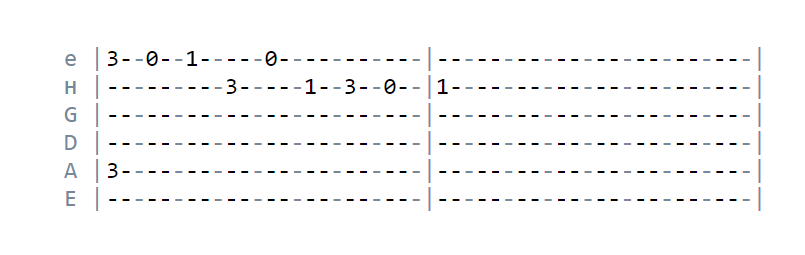
\includegraphics[scale=0.5]{../taby/kluziste.PNG}

\end{center}

	
\end{song}


\newpage	
\addcontentsline{toc}{section}{Knocking On Heaven\ap s Door}%\documentclass[../main.tex]{subfiles}


\begin{song}{title=\centering Knockin' On Heaven's Door \\\normalsize Bob Dylan  \vspace*{-0.3cm}}  %% sem se napíše jméno songu a autor
\moveright 4.5cm \vbox{      %Varianta č. 1  ---> Jeden sloupec zarovnaný na střed

\sloka
	^{G}Mama, ^{D}take this badge off of me ^{Ami} 
 
	^{G}I can't ^{D}use it ^{C}anymore. 
 
	It's gettin' dark, too dark for me to see.

	I feel like I'm knockin' on heaven's door.

\refren
	^{G}Knock, knock, ^{D}knockin' on heaven's  ^{Ami}door.

	^{G}Knock, knock, ^{D}knockin' on heaven's  ^{C}door. 
 
	Knock, knock, knockin' on heaven's door.

	Knock, knock, knockin' on heaven's door.

\sloka
	Mama, put my guns in the ground 

	I can't shoot them anymore. 

	That long black cloud is comin' down. 

	I feel like I'm knockin' on heaven's door. 

\refren

}
\setcounter{Slokočet}{0}
\end{song}
\begin{figure}[h]
\centering
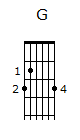
\includegraphics[width=3cm]{../Akordy/g}
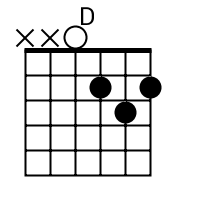
\includegraphics[width=3cm]{../Akordy/d}
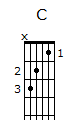
\includegraphics[width=3cm]{../Akordy/c}
\includegraphics[width=3cm]{../Akordy/Am}
\end{figure}
\newpage
\addcontentsline{toc}{section}{Kometa}\begin{song}{title=\centering Kometa \\\normalsize Jaromír Nohavica \vspace*{-0.3cm}}  %% sem se napíše jméno songu a autor
\moveright 1cm \vbox{      %Varianta č. 1  ---> Jeden sloupec zarovnaný na střed	
\begin{minipage}[t]{0.48\textwidth}\setlength{\parindent}{0.45cm}  %Varianta č. 2 --> Dva sloupce

\sloka 
	^{Ami{\color{white}\_}}Spatřil jsem kometu, oblohou letěla,
	
	chtěl jsem jí zazpívat, ona mi zmizela.
	
	^{Dmi{\color{white}\_}}Zmizela jako laň ^{G7}u lesa v remízku,
	
	^{C}v očích mi zbylo jen ^{E7}pár žlutých penízků.

\sloka
	Penízky ukryl jsem do hlíny pod dubem,
	
	až příště přiletí, my už tu nebudem.
	
	My už tu nebudem, ach, pýcho marnivá,
	
	spatřil jsem kometu, chtěl jsem jí 
	
	zazpívat.
	
\refren
	^{Ami}O vodě, o trávě, ^{Dmi}o lese,
	
	^{G7}o smrti, se kterou smířit ^{C\,\,\,\,\,\,}nejde se,
	
	^{Ami}o lásce, o zradě, ^{Dmi}o světě
	
	^{E}a o všech lidech, co kdy ^{E7}žili na téhle 
	
	 ^{Ami\,\,\,\,\,\,}planetě.
	
\sloka	
	Na hvězdném nádraží cinkají vagóny,
	
	pan Kepler rozepsal nebeské zákony,
	
	hledal, až nalezl v hvězdářských triedrech
	
	tajemství, která teď neseme na bedrech.

\sloka
	Velká a odvěká tajemství přírody,
	
	že jenom z člověka člověk se narodí,
	
	že kořen s větvemi ve strom se spojuje
	
	a krev našich nadějí vesmírem putuje.

\refren
Na na na\elipsa\dots

\sloka
	Spatřil jsem kometu, byla jak reliéf
	
	zpod rukou umělce, který už nežije,
	
	šplhal jsem do nebe, chtěl jsem ji osahat,
	
	marnost mne vysvlékla celého donaha.
	
\end{minipage}\begin{minipage}[t]{0.5\textwidth}\setlength{\parindent}{0.45cm}\vspace*{0.55cm}  % V případě varianty č.2 jde odsud text do pravé části

\sloka
	Jak socha Davida z bílého mramoru
	
	stál jsem a hleděl jsem, hleděl jsem nahoru.
	
	Až příště přiletí, ach, pýcho marnivá,
	
	my už tu nebudem, ale jiný jí zazpívá.


\refren
	O vodě, o trávě, o lese,
	
	o smrti, se kterou smířit nejde se,
	
	o lásce, o zradě, o světě,
	
	bude to písnička o nás a kometě\elipsa\dots

\end{minipage}
}
\setcounter{Slokočet}{0}
\end{song}


\newpage
\addcontentsline{toc}{section}{Kovárna}\begin{song}{title=\centering Kovárna \\\normalsize Tři sestry \vspace*{-0.3cm}}  %% sem se napíše jméno songu a autor
\moveright 4cm \vbox{      %Varianta č. 1  ---> Jeden sloupec zarovnaný na střed	

\sloka 
	^{A}Ve středu jsem na Kovárně, ^{C}ve čtvrtek jsem na Kovárně,

	^{F}i v pátek jsem na Kovárně, ^{G}v sobotu zas na Kovárně.
	
	Ve středu jsem na Kovárně, ve čtvrtek jsem na Kovárně,
	
	i v pátek jsem na Kovárně, v sobotu zas na Kovárně.

\sloka
	^{A}Můj dědek byl kovář ^{C}a má bába kovářka,

	^{D}muj strejda byl notář, ^{H}moje teta ^{C}notářka.
	
	Můj táta je kovář a má máma kovářka,
	
	muj brácha je notář a ségra je notářka.

\refren
	^{A}Středa, ^{C}čtvrtek, ^{D}pátek, ^{H}sobota a ^{C}neděle, 
	
	každej den jsem na Kovárně,	na Kovárně v Bráníku.

\sloka
	Vilu mám jen malou a v ní kupu dětí,
	
	umím jenom kovat, roky rychle letí,
	
	až já z toho umřu, na krchov mě nesou,
	
	na rakev mi dají půllitr mou milóóóůů.

\refren

\sloka
	Rakev mi ozdobí hustou bílou pěnou,
	
	syn se bude sklánět nad mou kovadlinou.
	
	Muj syn bude kovář, jeho žena kovářka
	
	a jejich syn notář, jejich dcera notářka.
	
	Už nebudu kovat, už nebudu kovat,
	
	všichni budou kovat, všichni budou kovat, jen já.

\refren

}
\setcounter{Slokočet}{0}
\end{song}\newpage
\addcontentsline{toc}{section}{Král a klaun}\begin{song}{title=\centering Král a klaun \\\normalsize Karel Kryl  \vspace*{-0.3cm}}  %% sem se napíše jméno songu a autor
\moveright 4cm \vbox{      %Varianta č. 1  ---> Jeden sloupec zarovnaný na střed	

\predehra
\textbf{G C G C G C}

\sloka 
	^{D}Král ^{C}do boje ^{G\,C}táh', ^{G} do ^{C{\color{white}\_\_}}veliké ^{G{\color{white}\_\_}}dálky, ^{C\,G}

	a s ^{C}ním do té ^{G{\color{white}\_\_}}války ^{D7}jel na mezku ^{G{\color{white}\_\_}}klaun,

	^{D}než ^{C{\color{white}\_\_}}hledí si ^{G\,C}stáh', ^{G} tak z ^{C{\color{white}\_\_\_}}výrazu ^{G\,\,}tváře ^{C\,G}

	^{C}bys nepoznal ^{G{\color{white}\_\_}}lháře, ^{D7}co zakrývá ^{G{\color{white}\_\_}}strach.

	^{D7}Tiše šeptal při té hrůze: ,,^{G{\color{white}\_\_}}Inter arma silent musae,''

	^{A}místo zvonku cinkal ^{{\color{white}\_\_\_\_}D7}brněním. ^{C#7\,D7}

	Král ^{C}do boje ^{G\,C}táh', ^{G} do ^{C{\color{white}\_\_}}veliké ^{G{\color{white}\_\_}}dálky,  ^{C\,G}

	^{C}a s ním do té ^{G{\color{white}\_\_}}války ^{D7}jel na mezku ^{G{\color{white}\_\_}}klaun.  ^{C\,G\,A7}

\sloka
	Král do boje táh', a sotva se vzdálil,
	
	tak vesnice pálil a dobýval měst,

	klaun v očích měl hněv, když sledoval žháře,

	jak smývali v páře prach z rukou a krev.
	
	Tiše šeptal při té hrůze: ,,Inter arma silent musae,''
	
	místo loutny držel v ruce meč.

	Král do boje táh', a sotva se vzdálil,
   
	tak vesnice pálil a dobýval měst.

\sloka
	Král do boje táh', s tou vraždící lůzou
	
	klaun třásl se hrůzou a odvetu kul,

	když v noci byl klid, tak oklamal stráže
	
	a, nemaje páže, sám burcoval lid.
	
	Všude křičel do té hrůzy, ve válce že mlčí Múzy,
	
	muži by však mlčet neměli.

	Král do boje táh', s tou vraždící lůzou

	klaun třásl se hrůzou a odvetu kul.

\sloka
	Král do boje táh', a v červáncích vlídných

	zřel, na čele bídných, jak vstříc jde mu klaun,

	když západ pak vzplál, tok potoků temněl,

	klaun tušení neměl, jak zahynul král:

	kdekdo křičel při té hrůze: ,,Inter arma silent musae,''

	krále z toho strachu trefil šlak.

	Klaun tiše se smál a zem žila dále
	
	a neměla krále, klaun na loutnu hrál,

	^{D7}klaun na loutnu ^{G}hrál, ^{D7}klaun na loutnu ^{G}hrál \ldots




}
\setcounter{Slokočet}{0}
\end{song}
\newpage
\addcontentsline{toc}{section}{Kutil}%\documentclass[../main.tex]{subfiles}

\begin{song}{title=\centering Kutil \\\normalsize Chinaski  \vspace*{-0.3cm}}  %% sem se napíše jméno songu a autor
\moveright 5cm \vbox{      %Varianta č. 1  ---> Jeden sloupec zarovnaný na stře

\sloka
Jsem ^{E}kutil. 

Mám malou ^{F#mi}dílnu víc mě ^{A{\color{white}\_\_}E}nezajímá, 

mé ^{E{\color{white}\_}}hobby je moje práce, 

šťastnej ^{F#mi}člověk každej ^{A}kdo to ^{{\color{white}\_}E}tak má. 

Mám ^{E}ženu. 

Je mladá ^{F#mi}krásná chytrá ^{A{\color{white}\_\_}E}přívětivá. 

Má jednu malinkatou ^{E{\color{white}\_}}chybu, 

že si ^{F#mi}se mnou vůbec ^{A{\color{white}\_\_}E}nepovídá.

\refren
A tak ^{F#mi}hledám holku sdílnou, 

co by chtěla kluka s dílnou, 

^{A}abych nebyl ^{H}sám. ^{H7} 

\textbf{E  F#mi  A  E  C#mi  A  G  D  E } 

\sloka
Jsem kutil. 

Mám malou dílnu víc mě nezajímá. 

Má práce je moje hobby, 

šťastnej člověk každej kdo to tak má. 

Mám ženu. 

Je mladá krásná chytrá přívětivá. 

Má jednu malinkatou chybu, 

že si se mnou vůbec nepovídá.

\refren

}
\setcounter{Slokočet}{0}
\end{song}
\newpage
\addcontentsline{toc}{section}{Lano co k nebi nás poutá}\begin{song}{title=\predtitle\centering Lano co k nebi nás poutá \\\large Traband  \vspace*{-0.3cm}}  %% sem se napíše jméno songu a autor
\begin{centerjustified}
\nejvetsi

\sloka
Já ^{F\z }sedával v přístavu, ^*{Gmi}popíj el kořalu, ^{F}s holkama ^{\z C7}laškoval.

A ^{F}bylo mi fuk, co je, ^{Gmi}hlavně když fajfka mi ^{F\z C7}doutná.

Co ^{F\,\,}bylo už není, ^*{Gmi}všech no mý jmění jsem ^{A7\,\,}dávno ^{\z Dmi}rozfofroval.

Jsme ^{F\,\,}silný, jak silný je ^{Gmi}lano, co k nebi nás ^{F C7 F}poutá.

\sloka
Ale najednou zmatek, když vešel ten chlápek, na mou duši! 

Objedná si drink a sedne si vedle do kouta.

Pak se nakloní ke mně a povídá jemně: \uv{Matouši!

Jsme silný, jak silný je lano, co k nebi nás poutá.}

\sloka
Já povídám: \uv{Pane, odkud se známe? Esli se nemýlíte?

A co je vám do mě, starýho mrchožrouta?}

On na to: \uv{Pojď, dej se na moji loď, má jméno \emph{Eternité}.} 

Jsme silný, jak silný je lano, co k nebi nás poutá.\\


^{Dmi D7}

\sloka
^{G}Ty jeho slova se ^{Ami\,\,\,}zařízly do mě ^{G\,\,\,\,}jako bys břitvou ^{D7\,\,\,\,\,\,}šmik,

^{G\,\,\,\,}jako když po ránu ^{Ami\,\,\,\,}vzbudí tě křik ^{G\,\,\,\,\, D7\,\,}kohouta.

^{G}Tak povídám: ,,Jdem!“ A ^{Ami}ještě ten den stal se ^{H7}ze mě ^{\,\,\,\, Emi}námořník. 

^{G}Jsme silný, jak silný je ^{Ami}lano, co k nebi nás ^{G D7 G}poutá.

\sloka
Tak zvedněme kotvy a napněme plachty, vítr začíná vát! 

Černý myšlenky vymeťme někam do kouta.

Hudba ať hraje o dobytí ráje, teď není čeho se bát.

/: Jsme silný, jak silný je lano, co k nebi nás poutá. :/\\

\end{centerjustified}
\setcounter{Slokočet}{0}
\end{song}
\newpage
\addcontentsline{toc}{section}{Leaving On A Jet Plane}\documentclass[../main.tex]{subfiles}

\chapter{Leaving on a jet plane}

\noindent \begin{minipage}{0.5\linewidth}
\begin{song}{title=Leaving on a jet plane}
\begin{verse}
All my bags^{C} are packed I'm ready^{F} to go\\
I'm standing^{C} here outside^{F} your door\\
I hate^{C} to wake you up^{F} to say goodbye^{G7} \\
But the dawn^{C} is breaking it's early^{F} morn\\
The taxi's^{C} waitin' he's blownin'^{F} his horn\\
Already^{C} I'm so lonesome^{F} I could die^{G7}\\
\end{verse}
\begin{verse*}
\hspace*{-0.45cm}\textbf{R:}So kiss^{C} me and smile^{F} for me\\
Tell^{C} me that you'll wait^{F} for me\\
Hold^{C} me like you'll never^{F} let me go^{G7} \\
Cause I'm^{C} leavin' on^{F} a jet plane\\
Don't^{C} know when I'll^{F} be back again\\
Oh,^{C} babe^{F}  I hate to go^{G7}\\
\end{verse*}
\begin{verse}
There's is many^{C} times I've let^{F} you down\\
So many^{C} time I've played^{F} around\\
I tell^{C} you now they^{F} don't mean a thing^{G7} \\
Every place^{C} I go I'll think^{F} of you \\
Every song^{C} I sing I'll sing^{F} for you \\
When I^{C} come back I'll bring^{F} your wedding ring^{G7} \\
\end{verse}
\end{song}
\end{minipage}
\begin{minipage}{0.5\textwidth}
\vspace*{-9.5cm}
\begin{song}{title=Leaving on a jet plane}
\begin{verse*}
\hspace*{-0.45cm}\textbf{R:}So kiss^{C}$\dots$
\end{verse*}
\begin{verse}
\item[3.]Now^{C} the time come^{F} to leave you \\
One^{C} more time let^{F} me kiss you \\ 
Then^{C} close your eyes I'll^{F} be on my way^{G7} \\
Dream^{C} about the days^{F} to come \\
When I^{C} won't have to leave^{F} alone \\
About the times I^{F} won't have to say^{G7} \\
\end{verse}
\begin{verse*}
\hspace*{-0.45cm}\textbf{R:}So kiss^{C}... \\
\end{verse*}
\end{song}
\end{minipage}\newpage
\addcontentsline{toc}{section}{Lemon Tree}%\documentclass[../main.tex]{subfiles}

\begin{song}{title=\centering Lemon Tree \\\normalsize Fool's Garden  \vspace*{-0.3cm}}  %% sem se napíše jméno songu a autor
\moveright 1cm \vbox{      %Varianta č. 1  ---> Jeden sloupec zarovnaný na střed	
\begin{minipage}[t]{0.48\textwidth}\setlength{\parindent}{0.45cm}  %Varianta č. 2 --> Dva sloupce

\sloka
I'm ^{Emi{\color{white}\_}}sittin' here in the ^{Hmi}boring room,

It's ^{Emi}just another rainy Sunday ^{Hmi}afternoon.

I'm ^{Emi{\color{white}\_\_}}wasting my time I got ^{Hmi}nothing to do,

I'm ^{Emi{\color{white}\_}}hangin' aroud I got ^{Hmi}waitin' for you.

But ^{Ami{\color{white}\_\_}}nothing ever happens^{H}

And I ^{Emi{\color{white}\_\_}}wonder.

\sloka
I'm drivin' aroud in my car,

I'm drivin' too fast, I'm drivin' too far,

I'd like to change my point of view,

I feel so lonely I'm waiting for you.

But nothing ever happens.

\refren
^{G}I wonder how, ^{D\,\,\,\,\,\,\,\,\,}wonder why

^{Emi{\color{white}\_\_}\,\,}Yesterday you told me 'bout the ^{Hmi}blue

 ^{\phantom{.}}blue sky

And ^{C}all that I can ^{D}see

Is just a yellow ^{G\,\,\,\,\,\,}lemon tree.^{D} 

I'm ^{G{\color{white}\_\_}}turnin' my head ^{D}up and down.

^{Emi}I'm turnin', turnin', turnin', ^{Hmi}turnin',

 ^{\phantom{.}}turnin' around

And ^{C}all that I can ^{D}see

Is just a yellow ^{G{\color{white}\_\_}}lemon tree.^{D} 

\sloka
^{4(Emi Hmi) Ami H Emi}Sing\,dip,\,ta\,da\,da\,dap\,di\,dap\,dam\elipsa.\elipsa.\elipsa.

\end{minipage}\begin{minipage}[t]{0.48\textwidth}\setlength{\parindent}{0.45cm}  % V případě varianty č.2 jde odsud text do pravé části
\vspace*{0.58cm}
\sloka
I'm sittin' here, I miss the power,

I'd like to go out, takin' a shower.

But there's a heavy cloud inside my head,

I feel so tired put myself into bed

Where nothing ever happens

And I wonder.

\sloka
^{H{\color{white}\_\_\_}}Isolation ^{Emi}is not good for me.

^{D{\color{white}\_\_\_}}Isolation, ^{G}I don't want to

^{H}sit on a lemon tree.

\sloka
I'm steppin' around in a desert of joy,

Baby, anyhow I get another toy

And everything will happen

And you'll wonder.

\refren
%^{G}I wonder how\elipsa\dots \\

\refren
%^{G}I wonder how\elipsa\dots \\


\dots\,and all that I can see --

and all that I can see --

and all that I can see 

Is just a yellow lemon tree.

\end{minipage}
}
\setcounter{Slokočet}{0}
\end{song}\newpage
\addcontentsline{toc}{section}{Let It Be}\begin{song}{title=\centering Let It Be \\\normalsize The Beatles  \vspace*{-0.3cm}}  %% sem se napíše jméno songu a autor
\moveright 4.8cm \vbox{      %Varianta č. 1  ---> Jeden sloupec zarovnaný na střed	

\sloka 
	When I ^{C\,\,}find myself in ^{G\,\,\,\,\,\,}times of trouble

	^{Ami\,\,\,\,}Mother Mary ^{Fmaj7\,\,}Comes to me
	
	^{C\,\,\,\,\,\,\,\,\,\,\,}Speaking words of ^{G\,\,\,\,\,\,\,\,\,\,}wisdom let it ^{F}be ^{C\,Dmi7\,C}
	
	^{C}And in my hour of ^{G\,\,\,\,\,\,\,\,\,\,}darkness

	She is ^{Ami\,\,\,\,}standing right in ^{Fmaj7}front of me

	^{C\,\,\,\,\,\,\,\,}Speaking words of ^{G\,\,\,\,\,\,\,\,\,\,}wisdom let it ^{F}be. ^{C\,Dmi7\,C}

\refren
	Let it ^{Ami}be let it ^{G}be let it ^{F}be let it ^{C}be

	^{C\,\,\,\,}Whisper words of ^{G\,\,\,\,\,\,\,\,\,\,}wisdom let it ^{F}be. ^{C\,Dmi7\,C}

\sloka
	And when the broken hearted people
   	
   	Living in the world agree
	
	There will be an answer let it be
   	
   	For though they may be parted
   	
   	There is still a chance that they will see
  	
  	There will be an answer let it be.

\moveright -0.2cm \vbox{\ssloka \textbf{R\textsubscript{2}:}
	Let it be let it be let it be let it be}
    
    There will be an answer let it be.

\refren


\refren

\sloka
	And when the night is cloudy
   	
   	There is still a light that shines on me
	
	Shine until the morrow let it be
   	
   	I wake up to the sound of music
   	
   	Mother Mary comes to me
   	
   	Speaking words of wisdom let it be.

\moveright -0.2cm \vbox{\ssloka \textbf{R\textsubscript{2}:}}


\moveright -0.2cm \vbox{\ssloka \textbf{R\textsubscript{2}:}}


}
\setcounter{Slokočet}{0}
\end{song}


\newpage
\addcontentsline{toc}{section}{Lilie}\begin{song}{title=\centering Lilie \\\normalsize Karel Kryl  \vspace*{-0.3cm}}  %% sem se napíše jméno songu a autor
\moveright 4cm \vbox{      %Varianta č. 1  ---> Jeden sloupec zarovnaný na střed	

\sloka 
	^{Dmi}Než zavřel bránu, oděl se do oceli, ^{A} a zhasil ^{Dmi{\color{white}\_}}svíci,  

	bylo už k ránu, políbil na posteli, ^{A} svou ženu ^{Dmi{\color{white}\_}}spící, 

	/: ^{F{\color{white}\_\_\_}}spala jak víla, ^{C\,\,}jen vlasy halily ji, 
	
	^{Dmi}jak zlatá žíla, ^{B}jak jitra v ^{A{\color{white}\_\_\_\_}}Kastilii, 
	
	^{Dmi{\color{white}\_\_}}něžná a bílá jak rosa na lilii, ^{B} ^{A}jak luna ^{Dmi{\color{white}\_}}bdící. :/ 

\phantom{tom}

(pískání) \textbf{Dmi\, B\, A\, Dmi\, B\, A\, Dmi}

\sloka
	Jen mraky šedé a ohně na pahorcích -- svědkové němí, 
	
	lilie bledé svítily na praporcích, když táhli zemí, 

	/: polnice břeskné vojácká melodie, 

	potoky teskné - to koně zkalili je, 
	
	a krev se leskne, když padla na lilie kapkami třemi. :/ 

\sloka
	Dozrály trnky, zvon zvoní na neděli a čas se vleče, 

	rezavé skvrnky zůstaly na čepeli u jílce meče, 
	
	/: s rukama v týle jdou vdovy alejemi, 

	za dlouhé chvíle zdobí se liliemi, 
	
	lilie bílé s rudými krůpějemi trhají vkleče. :/  



}
\setcounter{Slokočet}{0}
\end{song}
\newpage
\addcontentsline{toc}{section}{Made in Valmez}%\documentclass[../main.tex]{subfiles}

\begin{song}{title=\centering Made in Valmez \\\normalsize Mňága a Žďorp  \vspace*{-0.3cm}}  %% sem se napíše jméno songu a autor
\moveright 4cm \vbox{      %Varianta č. 1  ---> Jeden sloupec zarovnaný na střed	

\sloka
^{A{\color{white}\_}}Jako je sama skála, ^{D}tak jsem sám i ^{Hmi}já. ^{E} 

Jako je prázdná duha, tak jsem prázdný i já. 

Jako je zrádná voda, tak zradím i já. 

\refren
^{A{\color{white}\_\_\_\_\_}}Zkouším se prokopat ven -- zkouší se prokopat ven! 

^{D{\color{white}\_\_\_\_\_}}Zkouším se prokopat ven -- ^{Hmi{\color{white}\_}}zkouší se ^{A{\color{white}\_\_\_}}prokopat ven! 

^{A{\color{white}\_\_\_\_\_}}Zkouším se prokopat ven -- zkouší se prokopat ven! 

^{D{\color{white}\_\_\_\_\_}}Zkouším se prokopat ven! ^{Hmi\,\,\,A} 

\sloka
O půl třetí na náměstí ve Valašském Meziříčí 

jdu co noha nohu mine a každý sám sobě jsme stínem. 


\sloka
Nic mi není přitom melu z posledního, 

těžko říct o tom něco konkrétního. 

Stejná slova kolem stejný tváře 

a každý sám sobě jsme lhářem a já už zase. 

\refren

\refren

}
\setcounter{Slokočet}{0}
\end{song}
\newpage
\addcontentsline{toc}{section}{Měsíc}\begin{song}{title=\centering Měsíc \\\normalsize Mňága a Žďorp \vspace*{-0.3cm}}  %% sem se napíše jméno songu a autor
\moveright 4cm \vbox{      %Varianta č. 1  ---> Jeden sloupec zarovnaný na střed	

\sloka 
  ^{Emi{\color{white}\_}}Děkuju ti za to, ^{D}žes mi ^{G}ještě ^{{\color{white}\_}C}zavolala,  ^{G\,\,D}
  
  moje duše černá už to ani nečekala,
  
  jenže, moje drahá, je to všechno trochu na nic, 
  
  já už jsem se rozhod, zítra budu znovu panic. 

\sloka
  Děkuju ti za to, žes to rovnou nepoložil,
  
  že jsi nezapomněl, co jsi se mnou všechno prožil.
  
  Teď, když svítí měsíc pro každýho zvlášť, je mi to líto,
  
  jenže už je konec, však víš to. Vím to!

\sloka
  ^{Emi}Měsíc, ^{D\,\,G}\dots \, svítí ^{C{\color{white}\_\_\_}}Měsíc. ^{G\,\,D}

  Měsíc, \dots \, svítí Měsíc. 

  Měsíc, \dots \, svítí Měsíc. 

  Měsíc.


}
\setcounter{Slokočet}{0}
\end{song}


\newpage
\addcontentsline{toc}{section}{Milionář}%\documentclass[../main.tex]{subfiles}

\begin{song}{title=\centering Milionář \\\normalsize Jaromír Nohavica  \vspace*{-0.3cm}}  %% sem se napíše jméno songu a autor
\moveright 1cm \vbox{      %Varianta č. 1  ---> Jeden sloupec zarovnaný na střed	
\begin{minipage}[t]{0.48\textwidth}\setlength{\parindent}{0.45cm}  %Varianta č. 2 --> Dva sloupce

\sloka
^{D}U nás v domě ^{A}říkají mi Franta ^{D}Šiška

bo už od pohledu ^{G}chytry jsem jak ^{D}liška 

a dyž ^{A}kery něco neví 

nebo ^{D}dyž je na co levy  

tak de za ^{Emi}mnu a ja ^{A}všecko najdu v ^{D}knižkach 

\sloka
Raz mi říkal jeden znamy dole v baře 

že s tu hlavu moh bych do Milionaře 

čemu ne říkám si brachu 

šak má Železný dost prachu 

no a Čechovi se podíváš do tvaře 

\sloka
Dostal jsem se mezi partu uchazeču 

nikdo nemá šajnu jak tam nervy teču 

všecko viděl jsem do hnědě

tak jsem zmáčknul AbeCeDe 

no a už mě kruci ke stolečku vleču 

\sloka
Čech to začal takym malym interviju 

co pry robim esi kuřim a co piju 

tak jsem řeknul co jsem řeknul 

on se evidentně leknul 

a už začly blikat světla ve studiu

\sloka
to se přiznam nebylo mi vesele

První otázka pry co je ukulele 

tož tak jsem radši hlavu sklonil 

abych to všecko nezkonil 

říkám chtěl bych se obratit na přitele

\sloka
Lojza byl po hlasu silně nevyspaly 

asi zase celu šichtu prochlastali 

bylo slyšet jak tam dycha 

ale třicet vteřin ticha 

to je tak dyž se vam kamarad navali.

\sloka
Moju staru zatím doma braly mory 

lidi ohryzavali televizory 

tož padesat na padesat 

ať vím esi su to ty bulharské hory

\end{minipage}\begin{minipage}[t]{0.48\textwidth}\setlength{\parindent}{0.45cm}\vspace*{0.55cm}  % V případě varianty č.2 jde odsud text do pravé části


\sloka
A už jasně na tym komputuře sviti 

buďto je to za A vzacne lučni kviti 

nebo za Be nastroj strunny 

tu de kurňa o koruny 

a ja stejně jak na začatku jsem v řiti 

\sloka
Čech tam zatím maval tymi svymi čisly

tak si řikam Franta napij sa a mysli 

jake tudy sakypaky 

obratiš se na divaky

šak tu zatím za ty prachy enem kysli 

\sloka
Sam jsem byl zvědavy co publikum zvoli 

bo aj v obecenstvu možu sedět voli 

devadesat procent za Be 

ale to mi přišlo slabe 

bo co není stopro to mě dycky smali 

\sloka
Ještě že jsem chlap co zboja neutika 

říkam pane Čechu pujdem do rizika 

měl jsem v gaťach nadělano 

ale Čech zakřičel ano 

mate pravdu je to nastroj hudebnika

\sloka 
Lidi tleskali bo uspech to byl plny 

radosti zrobili dvě mexicke vlny 

a ja co mam srdce skromne 

jako všeci z Dolni Lomne 

jsem byl spokojeny bo sem ukol splnil 

\sloka
Pane Čechu nerad přetahnul bych strunu 

končim hru a beru tisicikorunu 

Čech se jenom chytnul stolu 

obočí mu spadlo dolu 

no a už se modry ku podlaze sunul 

\sloka
První třidu do Ostravy Intercity 

v jidelňaku celu cestu valim kyty 

a ta stovka co mi zbude 

to je přispěvek na chude 

bo Ostrava je region razovity.


\end{minipage}
}
\setcounter{Slokočet}{0}
\end{song}\newpage
\addcontentsline{toc}{section}{Muzeum}\begin{song}{title=\centering Muzeum \\\normalsize Jaromír Nohavica  \vspace*{-0.3cm}}  %% sem se napíše jméno songu a autor
\moveright 3cm \vbox{      %Varianta č. 1  ---> Jeden sloupec zarovnaný na střed	

\sloka
	^{D}Ve Slezském muzeu, ^{A}v oddělení ^{Hmi}třetihor
	
	je bílý ^{G}krokodýl a ^{Dmi}edvěd a liška a ^{A7}kamenní ^{D}trilobiti, ^{A7}
	
	^{D}chodí se tam jen tak, co ^{A}noha nohu ^{Hmi}mine, 
	
	abys viděl, jak ten ^{G}život plyne, ^{D}jaké je to všechno ^{A7}pomíjivé ^{D}živobytí,
	
	^{G}pak vyjdeš do parku a ^{D4sus}celou noc se ^{G}touláš noční Opavou

	a ^{C}opájíš se ^{G}představou, jaké to bude ^{D}v ^{G}ráji.
	

\refren
	V ^{D}pět třicet pět jednou z ^{A}pravidelných ^{Hmi}linek,
	
	sedm zastávek do ^{G}Kateřinek, ^{D}ukončete nástup, ^{A7}dveře se ^{D}zavírají.


\sloka
	Budeš-li poslouchat a nebudeš-li odmlouvat,
	
	složíš-li svoje maturity, vychováš pár dětí a vyděláš dost peněz,
	
	můžeš se za odměnu svézt na velkém kolotoči,
	
	dostaneš krásnou knihu s věnováním zaručeně,
	
	a ty bys chtěl plout na hřbetě krokodýla po řece Nil
	
	a volat: \uv{Tutanchámon, vivat, vivat!} po egyptském kraji.
	
\refren

\sloka
	Pionýrský šátek uvážeš si kolem krku,
	
	ve Valtické poručíš si čtyři deci rumu a utopence k tomu,
	
	na politém stole na ubruse píšeš svou rýmovanou Odysseu,
	
	nežli přijde někdo, abys šel už domů,
	
	ale není žádné doma jako není žádné venku, není žádné venku,
	
	to jsou jenom slova, která obrátit se dle libosti dají.

\refren

\sloka
	Možná si k tobě někdo přisedne,
	
	a možná to bude zrovna muž, který osobně znal Egypťana Sinuheta,
	
	dřevěnou nohou bude vyťukávat do podlahy rytmus metronomu,
	
	který tady klepe od počátku světa,
	
	nebyli jsme, nebudem a nebyli jsme, nebudem a co budem, až nebudem,
	
	jen navezená mrva v boží stáji.
	
	
\refren

}
\setcounter{Slokočet}{0}
\end{song}

\newpage
\addcontentsline{toc}{section}{Nagasaki Hirošima}\begin{song}{title=\predtitle\centering Nagasaki Hirošima \\\large Mňága \&  Žďorp  \vspace*{-0.3cm}}  %% sem se napíše jméno songu a autor
\begin{centerjustified}
\nejnejvetsi

\sloka
	^{A\z }Tramvají ^{E\z }dvojkou ^{D\z }jezdíval ^{E}jsem do ^*{\z A}Žideni c, ^{E\,\,D\,\,E}

	z ^{A}tak velký ^{E\z }lásky ^{D\z}většinou ^{E\z }nezbyde ^{F#mi\z }nic.~~~

	Z ^{D\z }takový ^{A\z}lásky ^{D\z}jsou kruhy ^{A\z}pod ^{{\color{white}\_}E}očima

	a dvě ^*{A}sp álený ^{E\z }srdce -- ^{D\z }Nagasaki ^{E\z}Hirošima. ^{A\,\,E\,\,D\,\,E}

\sloka
	Jsou jistý věci, co bych tesal do kamene,
	
	tam, kde je láska, tam je všechno dovolené
	
	a tam, kde není, tam mě to nezajímá.
	
	Jó dvě spálený srdce Nagasaki Hirošima.

\sloka
	Já nejsem svatej, ani ty nejsi svatá,
	
	jablka z ráje bejvala jedovatá,
	
	jenže hezky jsi hřála, když mi někdy byla zima.
	
	Jó dvě spálený srdce Nagasaki Hirošima.

\sloka
	Tramvají dvojkou jezdíval jsem do Židenic,
	
	z takový lásky většinou nezbyde nic.
	
	Z takový lásky jsou kruhy pod očima

	/: a dvě spálený srdce Nagasaki Hirošma. :/
	
	/: A dvě spálený srdce Nagasaki Hirošma. :/

\end{centerjustified}
\setcounter{Slokočet}{0}
\end{song}


\begin{figure}[h]
\predtitle\centering
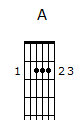
\includegraphics[width=3cm]{../Akordy/a.png}
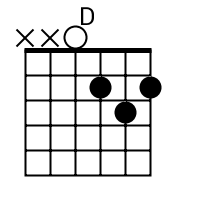
\includegraphics[width=3cm]{../Akordy/d.png}
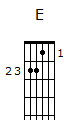
\includegraphics[width=3cm]{../Akordy/e.png}
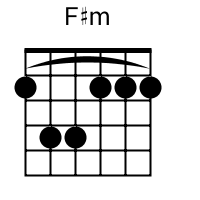
\includegraphics[width=3cm]{../Akordy/fxm.png}
\end{figure}
\newpage
\addcontentsline{toc}{section}{Nejlíp jim bylo}\begin{song}{title=\centering Nejlíp jim bylo \\\normalsize Mňága \& Žďorp  \vspace*{-0.3cm}}  %% sem se napíše jméno songu a autor
\moveright 5.5cm \vbox{      %Varianta č. 1  ---> Jeden sloupec zarovnaný na střed	

\sloka 
	Nejlíp jim ^{C\,Fmaj7}bylo,
	
	^{C}když ^{Fmaj7}nevěděli, co ^{C\,Fmaj7}dělaj, ^{C\,Fmaj7}
	
	jenom se ^{G}potkali 

	^{F}a neznělo to ^{C\,Fmaj}špatně. 

\sloka
	Tak se snažili 
	
	a opravdu si užívali,
	
	jenom existovali 
	
	a čas běžel skvěle.

\refren
	^{F}Nechám si projít ^{C}hlavou,
	
	^{G}kam všechny věci ^{Ami}plavou,
	
	^{F}jestli je všechno jen ^{C}dech

	^{G}tak jako kdysi v noci 

	^{Ami}spolu potmě na schodech. ^{C\,Fmaj7}

\sloka
	Pak se ztratili 

	a chvílema se neviděli,

	jenom si telefonovali 

	a byli na tom bledě.

\sloka
	A když se vrátili,
	
	už dávno nehořeli,

	jenom dál usínali

	chvíli spolu -- chvíli vedle sebe.

\refren

\sloka
	Nechej si projít hlavou,
	
	kam všechny věci věci plavou,
	
	jestli je všechno jen dech
	
	tak jako kdysi v noci 

	spolu potmě na schodech.



}
\setcounter{Slokočet}{0}
\end{song}
\newpage
\addcontentsline{toc}{section}{Orlice}\documentclass[../main.tex]{subfiles}

\chapter{Orlice}

\noindent
\begin{minipage}{0.5\linewidth}
\begin{song}{title=Orlice}


\begin{verse}[numbered]
	^{A}Orlice zas ^{E}šumí nad spla^{F#mi}vem \\
	Dodpusť mi ^{A}modlím se ať ^{E}všechno přesta^{C#mi}nem' \\
	odpusť mi ^{D}ke smutku ten ^{E}chlad \\
	je květen a ne listo^{F#mi}pad \\
	odpusť ^{A}modlím se když ^{E}spáváš na pra^{D}vém boku \\
\end{verse}

\begin{verse}[numbered]
	Když Orlice zas šumí nad splavem \\
	odpusť mi modlím se ať všechno přestanem' \\
	odpusť, že nemám na duši \\
	smutek ač králi Artuši \\
	prý utek' kůň i s bílým praporem\\
\end{verse}

\begin{verse}[numbered]
	^{C/G}Vysoko ^{G}v horách prší ^{A/E}kolem přelít ^{D}hvízdák \\
	Vysoko v horách prší na pyruších hnízda \\
	Vysoko v horách prší Dáša ruší, hvízdá \\
	Vysoko v horách horko v autobuse bonbon v puse ^{H}a ty hvízdáš s^{E} ní zdaleka \\
\end{verse}

\begin{verse}[numbered]
	Orlice zas šumí nad splavem \\
	odpusť mi modlím se ať všechno přestanem' \\
	odpusť ať nemám nikdy strach \\
	kéž dýchám na zobáčcích vah \\
	odpusť Orlice zas šumí nad splavem \\
\end{verse}

\end{song}
\end{minipage}
\begin{minipage}{0.5\textwidth}
\vspace*{-3.3cm}
\begin{song}{title=Orlice}
\begin{verse}
\item[5.]Vysoko v horách prší voda na tři couly\\ 
	Vysoko v horách prší Dáša už se choulí \\
	Vysoko v horách prší na kalhotách bouli \\
	Vysoko v horách horko v autobuse sucho v puse co si počneš s ní zdaleka \\
\end{verse}
\begin{verse}
\item[6.]Orlice zas šumí nad splavem \\
	odpusť mi modlím se ať všechno přestanem' \\
	odpusť, že nemám na duši smutek ač králi Artuši \\
	prý utek' kůň i s bílím praporem \\
\end{verse}
\begin{verse}
\item[7.]sólo
\end{verse}	
\begin{verse}
\item[8.]Orlice zas šumí nad splavem \\
	odpusť mi modlím se ať všechno přestanem' \\
	odpusť ať nemám vůbec strach \\
	kéž dýchám na zobáčcích vah \\
	odpusť Orlice zas šumí nad splavem\\
\end{verse}
\end{song}
\end{minipage}
\newpage
\addcontentsline{toc}{section}{Osmá barva duhy}\begin{song}{title=\centering Osmá barva duhy \\\normalsize Jaromír Nohavica  \vspace*{-0.3cm}}  %% sem se napíše jméno songu a autor
\moveright 1cm \vbox{      %Varianta č. 1  ---> Jeden sloupec zarovnaný na střed	
\begin{minipage}[t]{0.48\textwidth}\setlength{\parindent}{0.45cm}  %Varianta č. 2 --> Dva sloupce
\sloka
	^{Ami}Chladná jsou ^{Dmi}dubnová ^{Ami}rána ^{Dmi},
	
	^{Ami}ze slunce je ^{Dmi}vidět jenom ^{C\,E}kousek.
	
	^{Ami}Ve flašce ^{Dmi}od ^{Ami\,Dmi}činzána
	
	^{Ami}úhoři, ^{Dmi}úhoři ^{G}třou ^{Ami}se.
	
\refren
	^{Dmi}Všichni moji ^{Ami}známí
	
	^{F}spí, ^{Dmi}spí,	^{E}spí doma s manželkami.
	
	^{Dmi}Zůstali jsme ^{Ami}sami –- ^{E}já a ^{Ami}já.
	
	^{Ami}Města jsou jedno jako druhý,
	
	černá je osmá barva duhy.
	
	^{Dmi}Černá je barva, kterou ^{E}mám teď ^{Ami}nejraděj.
	
	Jó je to bída, je to bída,
	
	hledal jsem ostrov jménem Atlantýda
	
	^{Dmi}a našel vody ^{E}vody \dots vody ^{Ami}habaděj.
	
\sloka
	Kdyby měl někdo z vás zájem,
	
	uděláme velikánský mejdan.
	
	Pojedme tam a zpět rájem
	
	a svatej Petr bude náš strejda.

\refren

\sloka
	Pod okny řve někdo: \uv{Kémo,
	
	každý správný folkáč nosí vousy}.
	
	A já umím písničky jen v E moll
	
	a prsty jsem si až do masa zbrousil.
	
	Protože:
	
\end{minipage}\begin{minipage}[t]{0.48\textwidth}\setlength{\parindent}{0.45cm}\vspace*{0.55cm}  % V případě varianty č.2 jde odsud text do pravé části

\refren

\sloka
	Všichni moji známí
	
	teď spí, spí, spí doma s manželkami.

	Zůstali jsme sami -- já a vy.
	
	Města jsou jedno jako druhý,
	
	černá je osmá barva duhy.
	
	Černá je barva, kterou mám teď nejraděj.
	
	Jó, je to bída, je to bída,
	
	hledáme ostrov jménem Atlantida
	
	A nacházíme vody, vody, vody, vody,
	
	vody, vody, vody, vody, vody, vody,
	
	vody, vody, vody, vody, vody, vody,

	vody, vody habaděj. 

\end{minipage}
}
\setcounter{Slokočet}{0}
\end{song}
\newpage
\addcontentsline{toc}{section}{Ostravo}%\documentclass[../main.tex]{subfiles}

\begin{song}{title=\centering Ostravo \\\normalsize Jaromír Nohavica  \vspace*{-0.3cm}}  %% sem se napíše jméno songu a autor
\moveright \stred \vbox{      %Varianta č. 1  ---> Jeden sloupec zarovnaný na střed	

\refren
^{Dmi}Ostravo, Ostra^{A7}vo,

město mezi městy, ^{Dmi}hořké ^{A7}moje štěstí.

^{Dmi}Ostravo, Ostra^{A7}vo, 

černá hvězdo nad hla^{Dmi}vou.

\sloka
^{C}Pán Bůh rozdal jiným ^{F}městům všecku krásu, 

^{Gmi}parníky na řekách a ^{A7}dámy všité do atlasu. 

^{Dmi}Ostravo -- srdce ru^{A7}dé,

zpečetěný osu^{Dmi}ide. ^{A7}  ^{Dmi}

\refren

\sloka
Ať mě moje nohy nesly, kam mě nesly, 

ptáci na obloze jenom jednu cestu kreslí.

Ostravo - srdce rudé,

zpečetěný osude.

}
\setcounter{Slokočet}{0}
\end{song}
\newpage
\addcontentsline{toc}{section}{Ostravo}\begin{song}{title=\centering Otevřená zlomenina srdečního svalu \\\normalsize Wanastowi Vjecy \vspace*{-0.3cm}}  %% sem se napíše jméno songu a autor
\moveright 4.5cm \vbox{      %Varianta č. 1  ---> Jeden sloupec zarovnaný na střed	

\sloka 
	Jsem jako ^{G}vítr kterej zfoukne pírko ze tvejch dlaní,

	^{D}špínu jedný noci, jako hygiena ranní,

	^{Ami}velká voda slzí, který spláchnou noční hříchy, 

	^{C}tamburíny zvoní k ^{Es}operaci míchy.
	
	Narovnám ti páteř, poškrábu ti záda, 
	
	pofoukám ti srdce, zrada kamaráda

	lásky účel světí prostředky a smetí, 
	
	špínu jedný noci, který neuletíš.

	Otevřená zlomenina srdečního svalu, 
	
	trápení a kocovina, vůně tvýho žalu.
	
	Vypustíš svou hříšnou duši do slanýho moře, 
	
	neumírej děvče moje chti ti říct že:


\refren
	Ohořelou ^{G}károu chtěl bych dojet ^{D}ke hvězdám,

	který svítily z tvejch ^{Ami}očí dřív než ^{C}červotoči 

	se do tvýho srdce ^{F}daj, hm ^{D}hm.
	
	V ohořelym autě už dva měsíce nedejchám,
	
	sám se svojí vinou, už nikdy nechci jinou, 
	
	už asi nedoufám.

\sloka
	Pláčem solíš otevřený rány co se hojí, 
	
	tvoji krev i tělo příjímám pod obojí.

	Stejný lidi se soumrakem mají stejný stíny, 
	
	zmizelas jak před přízrakem, padám do hlubiny.
	
	Tvůj pramínek vlasů zaliju včelím voskem, 
	
	koukám na tu krásu a nechápu to mozkem.
	
	To co jsi mi dala já nikomu už nedám, 
	
	tak mi řekni má opičko proč tě marně hledám.

	Otevřená zlomenina srdečního svalu, 
	
	trápení a kocovina, vůně tvýho žalu.
	
	Vypustíš svou hříšnou duši do slanýno moře, 

	neumírej děvče moje chci ti říct, že:

\refren




}
\setcounter{Slokočet}{0}
\end{song}

\newpage
\addcontentsline{toc}{section}{Pangajó}%\documentclass[../main.tex]{subfiles}

\begin{song}{title=\centering Pangajó \\\normalsize \vspace*{-0.3cm}}  %% sem se napíše jméno songu a autor
\moveright 6cm \vbox{      %Varianta č. 1  ---> Jeden sloupec zarovnaný na střed	

\sloka
^{Ami}Pangajo, Pangajo
 
^{Dmi}ka mudi ^{Ami}ka

rodi ^{G}he rodi hu 

arong ^{Ami}baina ^{G}pondi ^{Ami}he  

te hu ^{G}a kema ^{Ami}o  

Te hu ^{G}a kema ^{Ami}o aó aó aó 

}
\setcounter{Slokočet}{0}
\end{song}
\newpage
\addcontentsline{toc}{section}{Partyzán}\begin{song}{title=\centering Partyzán  \\\normalsize Jaromír Nohavica  \vspace*{-0.3cm}}  %% sem se napíše jméno songu a autor
\moveright \stred \vbox{      %Varianta č. 1  ---> Jeden sloupec zarovnaný na střed	

\sloka 
	^{C}Když ^{C/H}přišli, bylo ^{Ami}léto,
	
	^{C}spálená pole ^{C/H}páchla ^{Ami}krví
	
	a kdo se vzdal, byl ^{G}ušetřen
	
	^{Dmi}a já vzal ^{F}zbraň do ^{C}rukou, ^{C/H}hm. ^{Ami}
	
\sloka
	Svoje pravé jméno už neznám,
	
	ženu nemám a syna také ne,
	
	a je nás víc podobných
	
	a naše oči hledí vpřed, hm.

\sloka
	Včera spali jsme v rozbité kůlně,
	
	 stará žena nám vařila polívku,
	
	ráno přišli vojáci,
	
	její dům hoří a ona v něm, hm.

\sloka
	Bylo nás osm, a jsme jen tři,
	
	bůhví, kolik nás bude zítra,
	
	ale jít musíme dál,
	
	hory jsou naše vězení, hm.
	
\sloka
	A vítr fouká, vítr fouká,
	
	nad lesy krouží bílí sokoli,
	
	den svobody se blíží,
	
	pak sejdem z hor do údolí, hm.

\sloka
Na na na \dots

\sloka =5. 


}
\setcounter{Slokočet}{0}
\end{song}


\newpage
\addcontentsline{toc}{section}{Perfect Day}\begin{song}{title=\centering Perfect Day \\\normalsize Lou Reed \vspace*{-0.3cm}}  %% sem se napíše jméno songu a autor
\moveright 2cm \vbox{      %Varianta č. 1  ---> Jeden sloupec zarovnaný na střed	
\begin{minipage}[t]{0.45\textwidth}\setlength{\parindent}{0.45cm}  %Varianta č. 2 --> Dva sloupce
\sloka 
	\textbf{E  Am  E  Am }

	^{Ami}Just a ^{D}perfect day, 

	^{G}Drink Sangria ^{C}in the park, 

	^{F}And then later, ^{Dmi}when it gets dark, 

	We go ^{E}home.
	 	
	^{Ami}Just a ^{D}perfect day, 

	^{G}Feed animals ^{C}in the zoo 

	^{F}Then later, ^{Dmi}a movie, too, 

	And then ^{E}home. 
 
 
\refren
	Oh ^{A}it's such a ^{D}perfect day, 

	I'm ^{C\# mi}glad I spent it with ^{D}you. ^{D\,\,D}

	^{A}Oh such a ^{E}perfect day, 

	You just ^{F\# mi}keep me ^{E}hanging ^{D}on, 

	You just ^{F\# mi}keep me ^{E}hanging ^{D}on. 
 
\sloka 
	Just a perfect day, 

	Problems all left alone, 

	Weekenders on our own. 

	It's such fun. 

	Just a perfect day, 

	You made me forget myself. 
	
	I thought I was someone else, 
	
	Someone good. 

\end{minipage}\begin{minipage}[t]{0.53\textwidth}\setlength{\parindent}{0.45cm}\vspace*{0.55cm}  % V případě varianty č.2 jde odsud text do pravé části

\refren 
	Oh it's such a perfect day, 
	
	I'm glad I spent it with you. 
	
	Oh such a perfect day, 
	
	You just keep me hanging on, 
	
	You just keep me hanging on. 
 

 
/: \textbf{F\# mi  E  D} :/

 
\sloka 
	/: ^{C\# mi}You're going to ^{G}reap 
	
	just what you ^{D}sow,  ^{D\,B\,A} :/
 
 	/: ^{C\# mi}You're going to ^{G}reap 
 	
 	just what you ^{D}sow,  ^{D\,B\,A} :/\\
 	
 	
\textbf{C\# mi   G   D   D   D   A }

\end{minipage}
}
\setcounter{Slokočet}{0}
\end{song}

\newpage
\addcontentsline{toc}{section}{Personal Jesus}\begin{song}{title=\centering Personal Jesus \\\normalsize Johny Cash  \vspace*{-0.3cm}}  %% sem se napíše jméno songu a autor
\moveright 1cm \vbox{      %Varianta č. 1  ---> Jeden sloupec zarovnaný na střed	

\begin{minipage}[t]{0.48\textwidth}\setlength{\parindent}{0.45cm}  %Varianta č. 2 --> Dva sloupce
%Pozn. písnička by se dala zapsat Da Capo formou, ale asi to uděláme jednodušší cestou a prostě to opíšeme
\sloka 
	Your ^{Emi}own, personal, Jesus,

	someone to hear your prayers,

	someone who ^{Am7\,G}cares.

	Your ^{Emi}own, personal, Jesus,

	someone to hear your prayers,

	someone who's ^{Am7\,G\,Emi}there.


\sloka
	^{Emi}Feeling unknown, and you're all alone,

	^{G}flesh and bone, by the ^{D}telephone,

	^{Am7}lift up the receiver,

	I'll ^{C}make you a ^{G}believer. ^{Emi}


\sloka
	^{Emi}Take second best, put me to the test,

	^{G}things on your chest, you ^{D}need to confess,

	^{Am7}I will deliver, you ^{C}know I'm a ^{G}forgiver. ^{Emi}


\refren %Pozn. v angličtině je to bridge, ale ten pojem v češtině neni, tak jsem řek refrén
/: ^{F#\,F}Reach out and touch ^{Emi}faith. :/



\sloka
	Your own, personal, Jesus,

	someone to hear your prayers,

	someone who cares.

	Your own, personal, Jesus,

	someone to hear your prayers,

	someone who cares.

\end{minipage}\begin{minipage}[t]{0.48\textwidth}\setlength{\parindent}{0.45cm}\vspace*{0.55cm}  % V případě varianty č.2 jde odsud text do pravé části

\sloka
	^{Emi}Feeling unknown, and you're all alone,

	^{G}flesh and bone, by the ^{D}telephone,

	^{Am7}lift up the receiver,

	I'll ^{C}make you a ^{G}believer, ^{Emi}

	^{Am7}I will deliver, you ^{C}know I'm a ^{G}forgiver. ^{Emi}


\refren
	/: ^{F#\,F}Reach out and touch ^{Emi}faith. :/

	/: ^{F#\,F}Reach out and touch ^{Emi}faith. :/
\end{minipage}
}
\setcounter{Slokočet}{0}
\end{song}

	\newpage
\addcontentsline{toc}{section}{Petěrburg}\begin{song}{title=\predtitle\centering Petěrburg  \\\large Jaromír Nohavica  \vspace*{-0.3cm}}  %% sem se napíše jméno songu a autor
\begin{centerjustified}
\nejnejvetsi

\sloka 
  ^{Ami}Když se snáší noc na střechy Petěrburgu, ^*{F}pa dá ^{E}na mě ^{Ami}žal,

  zatoulaný pes nevzal si ani kůrku ^*{F}ch leba, kterou ^*{E}js em mu ^{Ami}dal.

\refren
  /: ^*{C}Lá sku moji ^{Dmi\,\,\,}kníže ^{E}Igor si bere,
 
  ^{F{\color{white}\_}}nad sklenkou vodky ^{H7{\color{white}\_}}hraju ^{Adim\,\,}si ^{E}s revolverem,
  
  ^{Ami{\color{white}\_}}havran usedá na střechy Petěrburgu, ^{F{\color{white}\_}}čert ^{E}aby to ^{Ami}spral.

\sloka
  Nad obzorem letí ptáci slepí v záři červánků,
  
  moje duše, široširá stepi, máš na kahánku.

\refren
  /: Mému žalu na světě není rovno,
  
  vy jste tím vinna, Naděždo Ivanovno,
  
  vy jste tím vinna, až mě zítra najdou s dírou ve spánku. :/

\end{centerjustified}
\setcounter{Slokočet}{0}
\end{song}
\newpage
\addcontentsline{toc}{section}{Písnička pro Tebe}\begin{song}{title=\predtitle\centering Písnička pro Tebe \\\large Mňága a Žďorp  \vspace*{-0.3cm}}  %% sem se napíše jméno songu a autor
\begin{centerjustified}
\nejnejvetsi

\sloka
^{F\,}To je ta ^{C{\color{white}\_\_}G{\color{white}\_}}písnička pro te^{C\,}be 

^{F}z ^{C{\color{white}\_\_}\,\,G\,C}autobusáku,

^{{\color{white}\_\_}\,\,F}mrazivé ^{C}a modravé ^{G{\color{white}\_\_}}obrysy ^{C{\color{white}\_\_}}mraků 

^{F\,\,\,C\,\,}ptáků a ^{{\color{white}\_\_}G\,C}paneláků. 

\sloka
Nic není, co by stálo aspoň za něco 

a něco nestojí ani za to. 

Nic není, co by stálo aspoň za něco 

a něco nestojí ani za to. 

\sloka
Co za to stojí, to neví nikdo. 

Někdo možná snad, ale nikdo neví kdo. 

Co za to stojí, to neví nikdo. Nikdo. 

To je ta písnička pro tebe. 

\sloka = 1.

\sloka
/:Pro tebe\elipsa\dots\,:/ 

/:Pro tebe\elipsa\dots\,:/ 

/:Pro tebe\elipsa\dots\,:/ 

Pro tebe\elipsa\dots

\end{centerjustified}
\setcounter{Slokočet}{0}
\end{song}
\newpage
\addcontentsline{toc}{section}{Podzimní}\begin{song}{title=\predtitle\centering Podzimní \\\large Karel Plíhal  \vspace*{-0.3cm}}  %% sem se napíše jméno songu a autor
\begin{centerjustified}
\nejvetsi

\sloka
^*{A}Po dzimní obloha dala se ^{D}do gala, 

^*{E}ve černí vánek se do vlasů ^{A{\color{white}\_\_}}vplétá, 

a po tý obloze na křídle ^{D{\color{white}\_\_}}rogala 

s ^{E\,\,}tím vánkem ve vlasech Markéta ^{A{\color{white}\_}}létá.

\sloka
Nebe je modrý jako mý džíny, 

tak jsme si zpívali s klukama zamlada, 

zmizely smutky a podzimní splíny, 

prostě to všechno, co Markéta nerada. 

\sloka
Vysoko na nebe, hluboko do polí 

Markéta létá a přitom si zpívá, 

co oči nevidí, to srdce nebolí, 

je totiž podzim a brzo se stmívá. 

\sloka
Zmizely splíny a přívaly pláče 

a s nima ty protivný přízraky z minula,

připravte obvazy, dlahy a fáče, 

kdyby se náhodou se zemí minula. 

\sloka = 1.

\sloka = 2.

\sloka = 3.

\sloka = 4.

\sloka
/: Podzimní obloha dala se do gala, 

večerní vánek se do vlasů vplétá. :/ 

 Podzimní obloha dala se do gala, 
 
večerní vánek se do vlasů vplétá.

\end{centerjustified}
\setcounter{Slokočet}{0}
\end{song}
\newpage
\addcontentsline{toc}{section}{Převrat v Banánové republice} \documentclass[../main.tex]{subfiles}

\chapter{Převrat V Banánové Republice\\ \scalebox{0.8}[0.8]{Znouzecnost}}
\noindent\hspace{0.15\linewidth}\begin{minipage}{0.7\linewidth}
\begin{song}{title=Pangajó}

\begin{verse}[numbered]
^{F}Generál ^{C}Sancho ^{B}Grácia ^{C}zmocnil ^{F}se vlády ^{C} ^{B} ^{C} \\
v Banánový republice někde uprostřed pralesa. \\
Hlásili to po ránu ve zprávách a psali v novinách, \\
Banánová republika, kde není nic jinýho než banány ^{F}a ^{C}armáda ^{B} ^{C}
\end{verse}
\begin{verse*}
\hspace*{-0.45cm}\textbf{R:}  ^{Dmi}A já vám ^{B} řikam, že ^{C}z tohodle nekouká ^{F} zas nic ^{C} dobrý ^{Dmi} ho \\
^{Dmi}A já vám ^{B} říkam že ^{C} banány teď budou ^{F} zas o něco ^{C} dražší, ^{F}zas o něco ^{C}dražší ^{F} zas o něco ^{C} dražší^{B} ou ^{F}jééé.
\end{verse*}
\begin{verse}[numbered]
Generál Sancho Grácia stojí na balkóně \\
a hází po lidech slibama že bude líp. \\
A lidi vyskakují a lidi jsou rádi, \\
ale byli by radši, kdyby po nich házel koláče a řízky. \\
\end{verse}
\begin{verse*}
\hspace*{-0.45cm}\textbf{R:} 
\end{verse*}
\begin{verse}[numbered]
V Banánový republice je dneska hrozně veselo, \\
generála Sancha Gráciu hodili lidi z balkónu \\
a sním jeho poskoky a patolízaly, \\
a armáda složila zbrane, no to je veselo, veselo, veselo!
\end{verse}
\begin{verse*}
\hspace*{-0.45cm}\textbf{R:} 
\textbf{G  D  C  D}
\end{verse*}
\begin{verse}[numbered]
Dámy pánové, tá svržena vláda sedí momentálně v hostinci U exilu \\
a nalejvá si hlavy banánovým vínem a přemýšlí, \\
přemýšlí jak se dostat zpátky k moci.\\
No, když bude dost dlouho přemejšlet, tak určitě na něco přijde,\\
co třeba takhle vojensko-politický převrat!\\
\end{verse}
\end{song}
\end{minipage}\newpage
\addcontentsline{toc}{section}{Pyšný Janek} \begin{song}{title=\centering Pyšný Janek \\\normalsize Jaromír Nohavica  \vspace*{-0.3cm}}  %% sem se napíše jméno songu a autor
\moveright \stred \vbox{      %Varianta č. 1  ---> Jeden sloupec zarovnaný na střed	

\sloka 
	/: ^{G{\color{white}\_\_}}Pyšný Janku na okénku,

	pyšný v poli, ^{C\,\,\,\,\,}pyšný v ^{G\,\,\,\,\,\,\,}šenku. ^{C\,\,G} :/
	
	/:^{D{\color{white}\_}}Kajže ty si najdeš ženku,
	
	^{D{\color{white}\_}}kajže ^{Emi}ty si ^{C{\color{white}\_\_}}najdeš ^{G}ženku. :/ Jé.

\sloka
	/: Děvuchy do kola chodí,

	za ruky se spolu vodí. :/
	
	/: Ani jedna neuškodí,
	
	ani jedna neuškodí. :/ Jé.

\sloka
	/: Bo ty, švarný, pyšný Janku,
	
	nechceš žádnů za galánku. :/
	
	/: Inum koňa, inum šklanku,

	inum koňa, inum šklanku. :/ Jé.


}
\setcounter{Slokočet}{0}
\end{song}

\begin{figure}[h]
\centering
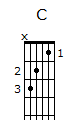
\includegraphics[scale=1.5]{../Akordy/c.png}
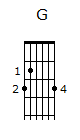
\includegraphics[scale=1.5]{../Akordy/g.png}
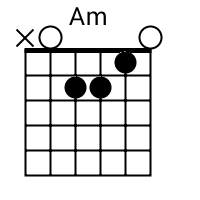
\includegraphics[scale=1.5]{../Akordy/am.png}
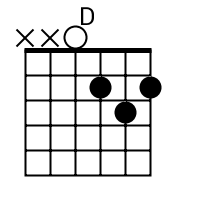
\includegraphics[scale=1.5]{../Akordy/d.png}
\end{figure}
\newpage
\addcontentsline{toc}{section}{Ráda se miluje}%\documentclass[../main.tex]{subfiles}

\begin{song}{title=\centering Ráda se miluje \\\normalsize Karel Plíhal  \vspace*{-0.3cm}}  %% sem se napíše jméno songu a autor
\moveright 4cm \vbox{      %Varianta č. 1  ---> Jeden sloupec zarovnaný na střed	

\refren
^{Hmi}Ráda se miluje, ^{A{\color{white}\_}}ráda ^{D}jí,

^{G{\color{white}\_}}ráda si ^{F#mi\,}jenom tak ^{Hmi{\color{white}\_}}zpívá, 

vrabci se na plotě ^{A\,{\color{white}\_}D\,}hádají, 

^{G{\color{white}\_\_}}kolik že ^{F#mi}času jí ^{Hmi{\color{white}\_}}zbývá.

\sloka
^{G}Než vítr dostrká k ^{D\,{\color{white}\_}}útesu ^{G}tu její legrační ^{{\color{white}\_}D\,\,F#mi}bárku 

a ^{Hmi\,\,}Pámbu si ve svým ^{A{\color{white}\_}D}notesu ^{G{\color{white}\_\_}}udělá ^{F#mi}jen další ^{Hmi\,\,}čárku.

\refren

\sloka
Psáno je v nebeské režii, a to hned na první stránce, 

že naše duše nás přežijí v jinačí tělesný schránce. 

\refren

\sloka
Úplně na konci paseky, tam, kde se ozvěna tříští, 

sedí šnek ve snacku pro šneky -- snad její podoba příští. 


\refren

}
\setcounter{Slokočet}{0}
\end{song}

\newpage
\addcontentsline{toc}{section}{Rád vařim}%\documentclass[../main.tex]{subfiles}

\newcommand\tab[1][1cm]{\hspace*{#1}}
\begin{song}{title=\centering Rád vařim \\\normalsize MIDI LIDI \vspace*{-0.3cm}}  %% sem se napíše jméno songu a autor
\moveright 1cm \vbox{      %Varianta č. 1  ---> Jeden sloupec zarovnaný na střed	
\begin{minipage}[t]{0.48\textwidth}\setlength{\parindent}{0.45cm}  %Varianta č. 2 --> Dva sloupce

\sloka
^{Gmi}Rád ^{Cmi\,\,\,\,}vařim a ^{Gmi\,\,}vim, že to ^{Cmi\,\,\,\,}umim

a ^{Gmi\,\,\,\,\,\,\,\,}holkám ^{Cmi}se to ^{Dmi}líbí.

\phantom{.}

Rád vařím a vím, že to umím

a holkám se to líbí.

\phantom{.}

Rád vařím a vím, že to umím

a holkám se to líbí.

\phantom{.}

Rád vařím a vím, že to umím

a holkám se to líbí.

\phantom{.}

[Mezihra]

\sloka
Rád vařím a vím, že to umím

a holkám se to líbí.

\phantom{.}

Rád vařím a vím, že to umím

a holkám se to líbí.

\phantom{.}

Rád vařím a holkám vařím 

a holkám se to líbí.

\phantom{.}

Já rád vařím a holkám vařím 

a holkám se to líbí.


\sloka
Rád vařím a holkám vařím
 
a holkám se to líbí.

\phantom{.}

Rád vařím a holkám vařím 

a holkám se to líbí.

\phantom{.}

Já vařím a holkám vařím
 
a holkám se to líbí.

\phantom{.}

Rád vařím a holkám vařím 

a holkám se to líbí.

\phantom{.}

[Mezihra]

\end{minipage}\begin{minipage}[t]{0.48\textwidth}\setlength{\parindent}{0.45cm}\vspace*{0.55cm}  % V případě varianty č.2 jde odsud text do pravé části

\sloka
Rád vařím a vím, že to umím

a holkám se to líbí.

\phantom{.}

Rád vařím a holkám vařím 

a moc se mi to líbí.

\phantom{.}

Rád mlčím a doma trčím 

ale v práci mi to myslí.

\phantom{.}

Rád mlčím a doma trčím 

ale v práci mi to myslí.

\phantom{.}

Rány hojím, a proto za to stojím

a Vám všem se to líbí.

\phantom{.}

Rány hojím, a proto za to stojím 

a Vám všem se to líbí.

\end{minipage}
}
\setcounter{Slokočet}{0}
\end{song}
\newpage
\addcontentsline{toc}{section}{Russian mystic pop IV.}\begin{song}{title=\centering Russian mystic pop IV. \\\normalsize Psí vojáci  \vspace*{-0.3cm}}  %% sem se napíše jméno songu a autor
\moveright 4cm \vbox{      %Varianta č. 1  ---> Jeden sloupec zarovnaný na střed	

\sloka 
	^{Ami{\color{white}\_}}Chodím po tom městě a ^{F{\color{white}\_\_\_}}nemám ani na tramvaj.
	
	^{G{\color{white}\_}}Není jaksi na místě, že ^{Ami}bych se z toho vyhrabal.
	
	^{Ami}Půjčil jsem si pětistovku a ^{F}od výčepu k báru
	
	^{G}jsem ji mezi prstama ^{{\color{white}\_}Ami}proměnil v mlžnou páru.
	
\refren
	/: Hej ^{Ami}hej \dots hej ^{F}hej \dots hej ^{G}hej \dots jsem ^{{\color{white}\_\_}Ami}mladej. :/
	
	 /:^{Gmi{\color{white}\_}}Připadá mi to děsný ale ^{D{\color{white}\_\_}}začíná mi bejt ^{F{\color{white}\_}}tohle město ^{C{\color{white}\_}}těsný. :/
	 
 	 ^{Gmi{\color{white}\_}}Připadá mi to děsný ale ^{D{\color{white}\_\_}}začíná mi bejt ^{F{\color{white}\_}}tohle město ^{C{\color{white}\_}}těsný. 

\sloka
	Ani šanci nemám, že bych se ráno nasnídal,
	
	příteli se ozvu na oběd se pozvu.
	
	Z hlediska věčnosti jsem plnej blbostí,
	
	subspecie ternitatis holky, holky -- Dakar Paris.

\refren

\sloka
	Až večer budu usínat, schoulím se do sebe
	
	a budu vzpomínat že měl jsem kdysi tebe.
	
	Nikdo už mi nezavolá nikdo už mě nepohladí,
	
	všem lidem totiž moje bytost vadí.

\refren

}
\setcounter{Slokočet}{0}
\end{song}\newpage
\addcontentsline{toc}{section}{Řekni, kde ty kytky jsou}\begin{song}{title=\centering Řekni\carka kde ty kytky jsou \\\normalsize Pete Seeger  \vspace*{-0.3cm}}  %% sem se napíše jméno songu a autor
\moveright 4cm \vbox{      %Varianta č. 1  ---> Jeden sloupec zarovnaný na střed	

\sloka 
  ^{C{\color{white}\_\_}}Řekni, kde ty ^{Ami}kytky jsou, ^{F}co se s nima ^{G{\color{white}\_\_\_}}mohlo stát,
  
  ^{C{\color{white}\_\_}}řekni, kde ty kytky ^{Ami}jsou, kde ^{Dmi{\color{white}\_}}mohou ^{G}být,

  ^{C{\color{white}\_\_}}dívky je tu ^{Ami{\color{white}\_}}během dne ^{D7{\color{white}\_\_}}otrhaly ^{G}do jedné,
  
  ^{F}kdo to kdy ^{C{\color{white}\_\_\_\_}}pochopí, ^{F}kdo to kdy ^{G{\color{white}\_\_\_}C\,\,\,}pochopí?

\sloka
  Řekni, kde ty dívky jsou, co se s nima mohlo stát,
  
  řekni, kde ty dívky jsou, kde mohou být,
  
  muži si je vyhlédli, s sebou domů odvedli,
  
  kdo to kdy pochopí, kdo to kdy pochopí?

\sloka
  Řekni, kde ti muži jsou, co se s nima mohlo stát,
  
  řekni, kde ti muži jsou, kde mohou být,
  
  muži v plné polní jdou, do války je zase zvou,
  
  kdo to kdy pochopí, kdo to kdy pochopí?

\sloka
  A kde jsou ti vojáci, co se s nima mohlo stát,
  
  a kde jsou ti vojáci, kde mohou být,
  
  řady hrobů v zákrytu, meluzína kvílí tu,
  
  kdo to kdy pochopí, kdo to kdy pochopí?

\sloka = 1.


}
\setcounter{Slokočet}{0}
\end{song}

\newpage %čárka v názvu?
\addcontentsline{toc}{section}{Sametová}\begin{song}{title=\centering Sametová \\\normalsize Žlutý pes  \vspace*{-0.3cm}}  %% sem se napíše jméno songu a autor
\moveright 4.5cm \vbox{      %Varianta č. 1  ---> Jeden sloupec zarovnaný na střed	

\sloka 
	^{G}Vzpomínám, když tehdá ^{C}před léty ^{G}začaly lítat ^{C}rakety,

	^{G}zdál se to bejt ^{C}docela dobrej ^{D}nápad,

	^{G}saxofony hrály ^{C}unyle, ^{C}frčely švédský ^{C}košile

	^{G}a někdo se moh' ^{Emi}docela dobře ^{C}flákat. ^{D}
	
\sloka
	 Když tam stál rohatej u školy, my neměli podepsaný úkoly,

	už tenkrát rozhazoval svoje sítě,

	poučen z předchozích nezdarů sestrojil elektrickou kytaru  
	
	a rock'n'roll byl zrovna narozený dítě.
	
\refren
	^{G}Vzpomínáš, takys' tu ^{D}žila, a ^{Emi}nedělej, že si ^{C}jiná,

	taková ^{G}malá pilná ^{D}včela, taková ^{C}celá ^{D}\ldots \, ^{G}sametová.
	
	
\sloka
	Přišel čas a jako náhoda byla tu bigbítová pohoda,
	
	kytičky a úsmevy sekretárok,
	
	sousedovic bejby Milena je celá blbá z Boba Dylana,
	
	ale to nevadí, já mám taky nárok.

\sloka
	Starý, mladý nebo pitomí mlátili do toho jako my,
	
	hlavu plnou Londýna nad Temží,
	
	a starej dobrej satanáš hraje u nás v hospodě mariáš
	
	a pazoura se mu trumfama jenom hemží.

\refren
	Vzpomínáš, už je to jinak, a jde z toho na mě zima,
	
	ty jsi, holka, tehdá byla taková celá \dots \,sametová.
	
\sloka
	A do toho tenhle Gorbačov, co ho znal celej Dlabačov,
	
	kopyta měl jako z Arizony,
	
	přišel a zase odešel a nikdo se kvůli tomu nevěšel
	
	a po něm tu zbyly samý volný zóny.

\refren
	Vzpomínáš, jak jsi se měla, když jsi nic nevěděla,
	
	byla to taková krásná cela a byla celá \dots
	 
	Vzpomínáš, jak jsi se měla, když jsi nic nevěděla,
	
	byla to taková krásná cela a byla celá \dots \,sametová.

}
\setcounter{Slokočet}{0}
\end{song}


\newpage
\addcontentsline{toc}{section}{Sarajevo}\begin{song}{title=\centering Sarajevo \\\normalsize Jaromír Nohavica \vspace*{-0.3cm}}  %% sem se napíše jméno songu a autor
\moveright \stred \vbox{      %Varianta č. 1  ---> Jeden sloupec zarovnaný na střed	

\sloka 
	^{Emi}Přes haličské pláně ^{Ami/F\# }vane vítr zlý,
	
	to ^{H7\,{\color{white}\_}}málo, co jsme měli, nám ^{Emi\,\,}vody sebraly
	
	jako tažní ptáci, ^{Ami/F\# }jako rorýsi
	
	^{H7\,{\color{white}\_}}letíme nad zemí, dva ^{Emi{\color{white}\_}}modré dopisy.

\refren
	^{Emi}Ještě hoří oheň a ^{Ami{\color{white}\_}}praská dřevo,
	
	^{D7/F\# }ale už je čas jít ^{G\,\,{\color{white}\_}}spát. ^{H7}

	^{Emi{\color{white}\_}}Tamhle za kopcem je ^{Ami{\color{white}\_\_}}Sarajevo,
	
	tam ^{H7\,\,\,\,\,\,\,\,\,\,}budeme se zítra ráno ^{Emi\,\,}brát.

\sloka
	Farář v kostele nás sváže navěky,
	
	věnec tamaryšku pak hodí do řeky,
	
	voda popluje zpátky do moře,
	
	my dva tady dole a nebe nahoře.

\refren

\sloka
	Postavím ti dům z bílého kamení,
	
	dubovými prkny on bude roubený,

	aby každý věděl, že jsem tě měl rád,
	
	postavím ho pevný, navěky bude stát.

\refren
	Ještě hoří oheň a praská dřevo,
	
	ale už je čas jít spát.
	
	Tamhle za kopcem je Sarajevo,
	
	tam zítra budeme se, lásko, brát\elipsa\dots


}
\setcounter{Slokočet}{0}
\end{song}

\newpage
\addcontentsline{toc}{section}{Sáro!}\begin{song}{title=\centering Sáro! \\\normalsize Traband  \vspace*{-0.3cm}}  %% sem se napíše jméno songu a autor
\moveright 1cm \vbox{      %Varianta č. 1  ---> Jeden sloupec zarovnaný na střed	
\begin{minipage}[t]{0.48\textwidth}\setlength{\parindent}{0.45cm}  %Varianta č. 2 --> Dva sloupce
\sloka 
	^{Ami\,}Sáro, ^{Emi\,}Sáro, ^{F}v noci se mi ^{C\,{\color{white}\_}}zdálo,

	že ^{F}tři andělé ^{C{\color{white}\_}}Boží k nám ^{F{\color{white}\_}}přišli na ^{G{\color{white}\_}}oběd.

	^{Ami\,}Sáro, ^{Emi\,}Sáro, jak ^{F\,\,}moc a nebo ^{C{\color{white}\_}}málo

	mi ^{F{\color{white}\_}}chybí abych ^{C{\color{white}\_}}tvojí duši ^{F\,{\color{white}\_}}mohl ^{\,\,\,G}rozumět?

\sloka
	Sbor kajícných mnichů jde krajinou v 
	
	tichu
	
	a pro všechnu lidskou pýchu
	
	má jen přezíravý smích.

	A z prohraných válek se vojska domů 
	
	vrací,
	
	však zbraně stále burácí
	
	a bitva zuří v nich.

\sloka
	Vévoda v zámku čeká na balkóně,
	
	až přivedou mu koně
	
	a pak mává na pozdrav.
	
	A srdcová dáma má v každé ruce růže.
	
	Tak snadno poplést může
	
	sto urozených hlav.

\sloka
	Královnin šašek s pusou od povidel
	
	sbírá zbytky jídel
	
	a myslí na útěk.
	
	A v podzemí skrytí slepí alchymisté
	
	už objevili jistě

	proti povinnosti lék.

	\end{minipage}\begin{minipage}[t]{0.48\textwidth}\setlength{\parindent}{0.45cm}\vspace*{0.55cm}  % V případě varianty č.2 jde odsud text do pravé části

\sloka
	Páv pod tvým oknem zpívá sotva procit
	
	o tajemstvích noci
	
	ve tvých zahradách.
	
	A já -- potulný kejklíř, co svázali mu ruce,

	teď hraju o tvé srdce
	
	a chci mít tě na dosah.

\sloka
	^{Ami\,}Sáro, ^{Emi\,}Sáro, ^{F\,{\color{white}\_\_}}pomalu a ^{C\,\,}líně

	
	^{F}s hlavou na tvém ^{C{\color{white}\_}}klíně ^{F{\color{white}\_}}chci se ^{{\color{white}\_\_}G}probouzet.
	
	^{F{\color{white}\_}}Sáro, Sáro, ^{C}Sáro, Sáro ^{F\,\,}rosa padá ^{C\,\,}ráno
	
	a ^{F}v poledne už ^{C{\color{white}\_\_}}možná ^{F{\color{white}\_}}bude jiný ^{G\,\,\,}svět.

	^{F{\color{white}\_}}Sáro, ^{C{\color{white}\_}}Sáro, ^{F{\color{white}\_\_}}vstávej, milá ^{C{\color{white}\_}}Sáro!

	^{F{\color{white}\_\_}}Andělé k nám ^{Dmi}přišli na ^{\,\,\,Cmaj7}oběd.


\end{minipage}
}
\setcounter{Slokočet}{0}
\end{song}

\newpage
\addcontentsline{toc}{section}{Slaboch Ben}\begin{song}{title=\centering Slaboch Ben \\\normalsize Kapitán Kid  \vspace*{-0.3cm}}  %% sem se napíše jméno songu a autor
\moveright 0.8cm \vbox{      %Varianta č. 1  ---> Jeden sloupec zarovnaný na střed	
\begin{minipage}[t]{0.48\textwidth}\setlength{\parindent}{0.45cm}  %Varianta č. 2 --> Dva sloupce

\sloka 
	^{C}V lesích ^{Ami}Ontaria ^{F}čerstvá smůla ^{G}voní.

	^{C}Tam, kde silných ^{A7}mužů paže ^{Dmi}vládne ^{G}jen,

	kde ^{C}sosny ^{Ami}staleté se ^{F}pod sekyrou ^{Cdim}kloní,

	v kempu ^{C}dřevorubců ^{G7}žije Slaboch ^{C}Ben.
	
\sloka
^{F}Mlčí stále ^{Cdim}jen a ^{C}snáší strasti ^{Ami}žití

a když ^{Dmi}kamarádů ^{G7}výsměch dávno ^{Ami}ztich.

^{E}V noci nad ^{Ami}jezerem, ^{Dmi}Polárka když ^{Ami}svítí,

^{E}odpouští jim věčný jejich smích.

\refren
	^{A}Že je slaboch, ^{A7}že prý nemá

	^{D}sílu, že se vrány bojí,

	^{E}říká o něm ^{E7}předák Andy ^{A}Renn.

	(Ten kojot) Hodí se jen ^{A7}k tomu, aby

	^{D}chodil kempu ^{D7}pro zásoby,

	^{E}je prý jenom ^{E7}pro smích Slaboch ^{A}Ben. ^{G7}

\sloka
	Na cestu mu dává bez nábojů zbraně,
	
	kdyby se snad před kojoty bránit chtěl.
	
	Kdyby se mu chtělo vystřelit si na ně,
	
	že by stejně, jak se míří nevěděl.
	
	Bez nábojů prý se aspoň nepostřelí,
	
	kdyby třeba přemoh strach a ránu dal.
	
	A když ještě dodal: "Snad se vrátíš celý,"
	
	kemp se málem smíchy rozsypal.
	
\refren
\end{minipage}\begin{minipage}[t]{0.48\textwidth}\setlength{\parindent}{0.45cm}\vspace*{0.59cm}  % V případě varianty č.2 jde odsud text do pravé části

\sloka
	Byli by se smáli ještě hodnou chvíli,
	
	kdyby tábor nebyl náhle přepaden
	
	bandou, kterou vedl jednooký Billy,
	
	kterým mnohý traper byl už zastřelen.
	
	Na pět kamarádů deset koltů cílí,
	
	každý z nich už s životem se rozžehnal.

	Když tu náhle výkřik zazní v pravou chvíli:
	
	\uv{Kdo se nevzdá, žít nebude dál!}
	
\refren
	To že je slaboch? Ten že nemá
	
	sílu, že se rány bojí,
	
	říká si teď v duchu Andy Renn.
	
	(Ten kojot) Ten že se nám hodí k tomu,
	
	aby chodil pro zásoby,
	
	tohle přece není slaboch Ben.

\sloka
	Deset koltů nato cíl svůj ihned mění,
	
	míří tam, kde v jejich zádech stojí Ben.

	Leč pět kamarádů v tomtéž okamžení
	
	střelbu spustí, dokud Bill je překvapen.
	
	Pak už v trávě leží jednooký Billy
	
	a s ním jeho čtyři muži mrtvi jen.
	
	Jako šestý s nimi s nenabitou zbraní,
	
	pro své pardy zemřel Slaboch Ben.

\refren
	Že je slaboch, že prý nemá
	
	sílu, že se vrány bojí,
	
	říkal o něm kdysi Andy Renn.
	
	Na hrobě, jenž teď ho kryje
	
	nápis je, že proto žije
	
	pardů pět, že zemřel pro ně Ben.
\end{minipage}
}
\setcounter{Slokočet}{0}
\end{song}

\newpage
\addcontentsline{toc}{section}{Slavíci z Madridu}%\documentclass[../main.tex]{subfiles}

\begin{song}{title=\centering Slavíci z Madridu \\\normalsize Waldemar Matuška \vspace*{-0.3cm}}  %% sem se napíše jméno songu a autor
\moveright 4.5cm \vbox{      %Varianta č. 1  ---> Jeden sloupec zarovnaný na střed	

\sloka
^{Ami}Nebe je ^{E}modrý a zlatý, ^{Ami}bílá sluneční záře,

horko a ^{E}sváteční šaty, ^{Ami}vřava a zpocený tváře,

vím, co ^{E}se bude dít, býk už ^{Ami}se v ohradě vzpíná,

kdo chce, ^{E}ten může jít, já ^{Ami}si dám sklenici vína.

\refren
^{Dmi}Žízeň je ^{Ami}veliká, život mi utíká,

^{E}nechte mě ^{Ami}příjemně snít,

^{Dmi}ve stínu pod ^{Ami}fíky poslouchat slavíky

^{E}zpívat si s ^{Ami}nima a pít.

\sloka
Ženy jsou krásný a cudný, mnohá se ve mně zhlídla,

oči jako dvě studny, vlasy jak havraní křídla,

dobře vím, co znamená pád do nástrah dívčího klína,

někdo má pletky rád, já si dám sklenici vína.

\refren

\sloka
Nebe je modrý a zlatý, ženy krásný a cudný,

mantily, sváteční šaty, oči jako dvě studny,

zmoudřel jsem stranou od lidí, jsem jak ta zahrada stinná,

kdo chce, ať mi závidí, já si dám sklenici vína.

\refren

}
\setcounter{Slokočet}{0}

\end{song}
\begin{figure}[h]
\centering
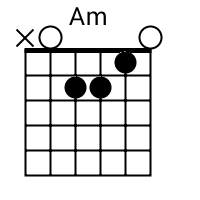
\includegraphics[scale=1.5]{../Akordy/am}
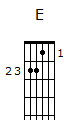
\includegraphics[scale=1.5]{../Akordy/e}
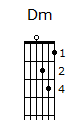
\includegraphics[scale=1.5]{../Akordy/dm}
\end{figure}

\newpage
\addcontentsline{toc}{section}{Sound Of Silence}%\documentclass[../main.tex]{subfiles}

\begin{song}{title=\centering Sound Of Silence \\\normalsize Simon \& Garfunkel  \vspace*{-0.3cm}}  %% sem se napíše jméno songu a autor
\moveright \stred \vbox{      %Varianta č. 1  ---> Jeden sloupec zarovnaný na střed	
\sloka
   ^{Ami}Hello darkness my ^{G}old friend
   
   I've come to talk with you ^{Ami}again
   
   because a ^{C}vision softly ^{F C}creeping
   
   left it seeds while I was ^{F C}sleeping.
   
   And the ^{F}vision that was planted in my ^{C}brain 
   
   still ^{Ami}remains ^{C}within the ^{G}sound of ^{Ami}silence.

\sloka
   In restless dreams I walked alone, 
   
   narrow streets of cobble-stone ,
   
   'neath the halo of a street lamp 
   
   I turned my collar to the cold and damp.
   
   When my eyes were stabbed by the flash of a neon light 
   
   that spilt the night and touched the sound of silence.
   
\sloka
   And in the naked light I saw 
   
   ten thousand people maybe more 
   
   People talking without speaking,
   
   people hearing without listening,
   
   people writing songs that voices never share,
   
   and no one dare disturb the sound of silence.
   
\sloka
   \uv{Fools!} said I \uv{you do not know
   
   silence like a cancer grows 
   
   hear my words that I might teach you 
   
   take my arms that I might reach you.} 
   
   But my words like silent raindrops fell 
   
   and echoed in the wells of silence. 
   
\sloka
   And the people bowed and prayed 
   
   to the neon god they made 
   
   and the sign flashed out its warning 
   
   in the words that it was forming and the sign said: 
   
   \uv{The words of the prophets are written on the subway walls 
   
   and tenament halls} and whisper'd in the sound of silence. 
   

}
\setcounter{Slokočet}{0}
\end{song}
\newpage
\addcontentsline{toc}{section}{Space Oddity}\begin{song}{title=\predtitle\centering Space Oddity \\\large David Bowie  \vspace*{-0.3cm}}  %% sem se napíše jméno songu a autor

\nejvetsi
\begin{centerjustified}

\sloka 
	^{C\z}Ground control to Major ^{Emi\z}Tom, ^{C\z}Ground control to Major ^{Emi\z}Tom:

	^{Ami}Take your ^{Am7/G\z}protein~pills and ^{D7}put your helmet on.

	^{C\z}Ground control to Major ^{Emi\,}Tom:  ^{C\z}Commencing countdown engine's ^{Emi\z}on~~

	^{Ami\z}Check ^{Ami7/G}ignition and may ^{D7\,\,}God's love be with you

	^{C\z }This is ground control to Major ^{E7}Tom, you've really made the ^{F\z}grade!

	And the ^{Fmi\z }papers want to ^{C\z }know whose shirts you ^{F\z}wear,

	now it's ^{Fmi\,}time to leave the ^{C{\color{white}\_\_}}capsule if you ^{F{\color{white}\_}}dare.

	^{C{\color{white}\_}}This is Major Tom to ground ^{\,E7}control, I'm stepping through the ^{F{\color{white}\_}}door

	And I'm ^{Fmi{\color{white}\_}}floating in the ^{C\z}most peculiar ^{F\,\,\,}way 

	and the ^{Fmi\,}stars look very ^{C\z}different ^{F}today

	For ^{Fmaj7}here am I ^{Em7}sitting in a tin ^{Fmaj7\:}can,~far~above the ^{Em7}world

	^{Bmaj7}Planet Earth is ^{Ami}blue and there's ^{G{\color{white}\_\_\_}}nothing I can ^{F}do.

	\phantom{.}

	\phantom{.}

/: \textbf{C\,F\,G\,A} :/ \textbf{Fmaj7\,Em7\,A\,C\,D\,E}

\end{centerjustified}
\newpage
\begin{centerjustified}

\sloka
	^{C{\color{white}\_\_\_}}Though I'm passed one hundred thousand ^{E7{\color{white}\_}}miles, I'm feeling very ^{F\,\,}still

	And I ^{Fmi\,}think my spaceship ^{C\,{\color{white}\_\_}}knows which way to ^{F}go,

	tell my ^{Fmi}wife I love her ^{C\,\,\,}very much, she ^{F{\color{white}\_\_}}knows.

	^{G\z}Ground control to ^{E7\,\,}Major Tom:

	Your ^{Ami{\color{white}\_}}circuit's dead, there's ^{Am7/G\,\,\,}something wrong.

	Can you ^{D7\,\,}hear me Major Tom? Can you ^{C\,\,}hear me Major Tom? 

	Can you ^{G\,\,}hear me Major Tom? Can you\dots

	^{Fmaj7\z}Here~am I ^{Emi7\,\,}floating in my tin ^{Fmaj7\,}can,~far~above the ^{Emi7}moon.

	^{Bmaj7}Planet Earth is ^{Ami}blue and there's ^{G\z}nothing I can ^{F}do.


\end{centerjustified}
\setcounter{Slokočet}{0}
\end{song}
\newpage
\addcontentsline{toc}{section}{Strom kýve pahýly}\begin{song}{title=\centering Strom kýve pahýly \\\normalsize Divadlo Sklep \vspace*{-0.3cm}}  %% sem se napíše jméno songu a autor
\moveright 4cm \vbox{      %Varianta č. 1  ---> Jeden sloupec zarovnaný na střed	

\sloka
	^{A{\color{white}\_}}Když slunce ^{Hmi7{\color{white}\_}\,\,}zapadá, tak ^{A{\color{white}\_}}moje ^{{\color{white}\_}D}nálada ^{E7} ^{\,\,\,\,A}klesá, ^{Hmi7\,\,A\,\,D\,\,E7}

	^{A{\color{white}\_}}strom kýve ^{Hmi7{\color{white}\_}\,\,}větvemi, ^{A}přítelem on je ^{D}mi, ^{Emi7} ^{\,\,\,\,\,A}plesá, ^{Hmi7\,\,A\,\,D\,\,E7}

	^{A}já však mám v duši žal, čert ^{Hmi7}ví, kde se tam vzal,

	^{\,\,A}tepe, ^{{\color{white}\_\_}Hmi7}tepe, ^{\,\,A}tepe, ^{\,\,D}tepe. ^{E7}

\refren
	^{A{\color{white}\_\_}}Strom kýve ^{Hmi7\,\,\,}pahýly, chtěl ^{A{\color{white}\_}}bych jen na ^{{\color{white}\_}\,D}chvíli tebe,

	^{A{\color{white}\_\_}}strom kýve ^{Hmi7\,\,\,}pahýly, chtěl ^{A{\color{white}\_}}bych jen na ^{{\color{white}\_}\,D}chvíli tebe,

	^{A{\color{white}\_}}rosu mám v ^{Hmi7{\color{white}\_\_}}kanadách, v mých ^{A{\color{white}\_\_\_}}černých ^{{\color{white}\_\_}D}kanadách zebe,

	^{A{\color{white}\_}}rosu mám v ^{Hmi7{\color{white}\_\_}}kanadách, v mých ^{A{\color{white}\_\_\_}}černých ^{{\color{white}\_\_}D}kanadách zebe.


\sloka
	Znám dobře kůru lip, té dal jsem kdysi slib mlčení,

	znám řeč, jíž mluví hřib, sám jako jedna z ryb jsem němý,

	však lesy, ty mám rád, tam cítím se vždycky mlád,

	vždycky líp, vždycky líp, vždycky líp, vždycky líp.



\refren

\phantom{.}

   /: Strom kýve pahýly, chtěl bych jen na chvíli tebe :/ 4x


}
\setcounter{Slokočet}{0}
\end{song}\newpage
\addcontentsline{toc}{section}{Své Rocky Mountains}\begin{song}{title=\centering Své Rocky Mountains \\\normalsize Vojta Kidák Tomáško  \vspace*{-0.3cm}}  %% sem se napíše jméno songu a autor
\moveright \stred \vbox{      %Varianta č. 1  ---> Jeden sloupec zarovnaný na střed	

\sloka 
	Je ^{A{\color{white}\_\_\_}}srpnový pátek a na horách sněží,

	^{D{\color{white}\_\_}}někdo jde vzhůru, někdo si věří,
	
	^{A{\color{white}\_\_}}krosna na zádech ^{D}tíží jak žulový ^{A{\color{white}\_}}blok.
	
	^{\phantom{.}}Zatím, co dole je léto a stromy
	
	a ^{D{\color{white}\_\_}}silácké řeči těch co se bojí,
	
	^{A}do bílé pláně ^{D{\color{white}\_\_}}udělat první ^{A{\color{white}\_}}krok.

\refren

\sloka
	^{D{\color{white}\_\_\_}}Vždycky se najdou a ^{G{\color{white}\_\_}}znovu to zkouší
	
	^{D{\color{white}\_\_}}slunce jak plamen ^{A{\color{white}\_}}bodá je v očích,
	
	^{E{\color{white}\_}}rvou se jak koně, ^{D}jen aby našli své ^{A}já.

\sloka	
	Sklonil jsem hlavu a ptal se sám sebe,
	
	jestli jak oni mám to svoje nebe
	
	tak blízko na dosah a nejsem na kolenou.
	
	Bez velkých řečí a ohraných frází,
	
	vstával jsem do tmy a nejmíň mi schází
	
	publikum, co chce mít za každou cenu své šou.

\refren

\sloka
	Možná mám poslední, poslední šanci,
	
	vzít svoji víru a v ledovém tanci
	
	na vrchol vynést svou vlajku a vidět ji vlát.
	
	Má každý před sebou své Rocky Mountains,
	
	svůj kopec z dětství, co zdál se být zlatý,
	
	ale kolik jich ztratilo cepín a muselo vzdát. 

\refren

\refren

\refren


}
\setcounter{Slokočet}{0}
\end{song}


\newpage
\addcontentsline{toc}{section}{To ta He\v lpa}\begin{song}{title=\centering To ta He\v lpa \\\normalsize  \vspace*{-0.3cm}}  %% sem se napíše jméno songu a autor
\moveright 4cm \vbox{      %Varianta č. 1  ---> Jeden sloupec zarovnaný na střed	

\sloka 
	^{Dmi}To ta ^{G{\color{white}\_\_}}Helpa, ^{Dmi}to ta ^{G{\color{white}\_\_}}Helpa, ^{Dmi\,}to je ^{A7{\color{white}\_\_}}pekné ^{Dmi\,\,}mesto.

	^{Dmi}A v tej ^{G{\color{white}\_\_}}Helpe, ^{Dmi}a v tej ^{G{\color{white}\_\_}}Helpe ^{Dmi\,{\color{white}\_\_}}švarných ^{A7{\color{white}\_\_\_}}chlapcov ^{Dmi}je sto.

	/: ^{B{\color{white}\_\_}}Koho ^{C7}je sto, ^{F\,\,{\color{white}\_}}toho je sto, ^{C}nie po mojej ^{\,\,\,F\,\,A7}vóli,

	^{Dmi}len za ^{G{\color{white}\_\_\_}}jednym, ^{Dmi}len za ^{G{\color{white}\_\_\_}}jednym ^{Dmi\,A7{\color{white}\_\_}}srdiečko ma ^{Dmi}boli. :/


\sloka
	Za Janíčkom, za Palíčkom krok by něspravila,
	
	za Ďuríčkom, za Mišíčkom Dunaj preskočila.

	/: Dunaj, Dunaj, Dunaj, Dunaj, aj to širé pole,
	
	len za jedním, len za jedním, počešenie moje. :/


}
\setcounter{Slokočet}{0}
\end{song}


\newpage
\addcontentsline{toc}{section}{Traktor}\begin{song}{title=\predtitle\centering Traktor \\\large Visací zámek \vspace*{-0.3cm}}  %% sem se napíše jméno songu a autor
\begin{centerjustified}

\begin{varwidth}[t]{0.5\textwidth}\setlength{\parindent}{0.45cm}  % V případě varianty č.2 jde odsud text do pravé části

\sloka
^{F\z}Jede ^{\z As\:\:\:\:}traktor,~je~to Zetor,

^{B\z}jede do hor ^{F\z}orat brambor.

\sloka
Zemědělci brambor zasejí,

potom pohnojí, pak zas vyrejí.

Mládenec si kapsu namastí,

prachama zachrastí

na děvu povětrnou.

\refren

/: ^{F{\color{white}\_\_\_}As\,}Kriminalita, ^{F{\color{white}\_\_\_}As\,}kriminalita,
^{F{\color{white}\_\_\_}As\,}kriminalita, 

^{B\z}mládeže. :/

\sloka
Mládenec a děva spolu jdou

před novou hospodou, hrozně se radujou.

Nejdřív se tu spolu opijem,

družstevní prase zabijem

a pak si užijem.

\refren

\sloka
Mládenec se hrozně opije,

vepříka zabije a pak se vzapamatuje.

Svýho čimu ihned lituje,

za mříže putuje

i s děvou povětrnou.

\refren

\sloka
Jede traktor, je to Zetor,

jede do hor orat brambor.

\end{varwidth}\mezisloupci

\end{centerjustified}
\setcounter{Slokočet}{0}
\end{song}
\newpage
\addcontentsline{toc}{section}{Trezor}\begin{song}{title=\centering Trezor \\\normalsize Karel Gott  \vspace*{-0.3cm}}  %% sem se napíše jméno songu a autor
\moveright 3cm \vbox{      %Varianta č. 1  ---> Jeden sloupec zarovnaný na střed	

\sloka 
	^{D}Ze zdi na mě tupě zírá ^{G}po trezoru temná díra,

	^{E7{\color{white}\_\_\_}}poznám tedy bez nesnází, ^{A7}že tam nepochybně něco schází.

	^{D}Ve zdi byl totiž po dědovi ^{G{\color{white}\_}}velký trezor ocelový.

	^{A7{\color{white}\_}}Mám tedy ztrátu zdánlivě ^{{\color{white}\_\_\_}D}minimální.
      
\sloka
	^{D}Na to že ^{A7{\color{white}\_\_\_}}náhodně v krámě vášnivé dámě ^{D{\color{white}\_}}padl jsem za ^{Hmi}trofej,

	^{E7{\color{white}\_\_}}tvrdila pevně: ,,Přijdu tě levně, ^{A7{\color{white}\_\_\_}}nezoufej!`` Ó jé, jé, jé, jé.

	^{D{\color{white}\_\_}}Jenže potom v naší vile ^{G{\color{white}\_\_\_}}chovala se zhůvěřile,

	^{E7}aby měla správné klima, ^{A7}dal jsem ji do trezoru, ať v klidu dřímá.
      
\refren
	^{D{\color{white}\_\_\_}}Spánku se bráním už noc pátou, ^{G}ne ale žalem nad tou ztrátou,

	^{A7}jen hynu bázní, že kasař úlovek ^{G D}vrátí.
      
\sloka = 2.
      
\refren


}
\setcounter{Slokočet}{0}
\end{song}

\newpage
\addcontentsline{toc}{section}{Tu kytaru jsem koupil kvůli tobě}\begin{song}{title=\predtitle\centering Tu kytaru jsem koupil kvůli tobě \\\large Václav Neckář \vspace*{-0.3cm}}  %% sem se napíše jméno songu a autor
\begin{centerjustified}
\nejnejvetsi

\ssloka{} ^{A}Jak můžeš bejt tak ^{F#mi\,\,}krutá, 

	^{Hmi\z}copak nemáš kouska citu v ^{E\z}těle.

\sloka                                                               
	^{A}Tu kytaru jsem koupil kvůli tobě 
                                   
	a dal jsem za ni celej tátův ^{E\z}plat,
                               
	ta ^{A\z}dávno ještě byla ve ^{D}výrobě 
	
	a já už ^{A\z}věděl ^{E}co ti budu ^{A\z}hrát.

\sloka
	To ještě rostla v javorovém lese 
	
	a jenom vítr na to dřevo hrál,

	a já už trnul, jestli někdy snese, 
	
	žár, který ve mně denně narůstal.

\sloka
	S tou kytarou teď stojím před tvým domem, 
	
	měj soucit aspoň k tomu javoru,

	jen kvůli tobě přestal býti stromem, 
	
	tak už nás oba pozvi nahoru.

	Pozvi nahoru, pozvi nahoru.

\end{centerjustified}
\setcounter{Slokočet}{0}
\end{song}
\newpage
\addcontentsline{toc}{section}{Už to nenapravím}\begin{song}{title=\centering Už to nenapravím \\\normalsize Jaroslav Samson Lenk  \vspace*{-0.3cm}}  %% sem se napíše jméno songu a autor
\moveright 1.2cm \vbox{      %Varianta č. 1  ---> Jeden sloupec zarovnaný na střed	

\refren /: ^{Ami}Vap tada dap\elipsa\dots ^{D\,\,F\,\,E} :/

\sloka
	V ^{Ami}devět hodin dvacet pět mě ^{D{\color{white}\_\_\_}}opustilo štěstí, 
	
	ten ^{F{\color{white}\_}}vlak, co jsem jím měl jet, na koleji ^{E{\color{white}\_\_}}dávno ^{E7{\color{white}\_}}nestál.
	
	V ^{Ami}devět hodin dvacet pět ^{D{\color{white}\_}}jako bych dostal pěstí,
	
	já ^{F}za hodinu na náměstí měl jsem ^{E{\color{white}\_}}stát, ale ^{E7}v jiným městě.
	
	
	Tvá ^{Ami}zpráva zněla prostě a byla tak krátká,
		
	že ^{Dmi{\color{white}\_}}stavíš se jen na skok, že nechalas mi vrátka ^{G{\color{white}\_\_}}zadní otevřená, ^{E{\color{white}\_\_}}zadní otevře^{E7}ná.
	
	Já ^{Ami{\color{white}\_}}naposled tě viděl když ti bylo dvacet 
	
	a ^{Dmi}to si tenkrát řekla, že už se nechceš vracet, ^{G}že si unavená, ^{E}ze mě unave^{E7}ná.
	


\refren

\sloka
	Já čekala jsem, hlavu jako střep a zdálo se, že dlouho, 
	
	snad může za to vinný sklep, že člověk často sleví.
	
	Já čekala jsem, hlavu jako střep, podvědomou touhou, 
	
	já čekala jsem dobu dlouhou víc než dost, kolik přesně nevím.


	Pak jedenáctá bila a už to bylo passé, 

	já dřív jsem měla vědět, že vidět tě chci zase, že láska nerezaví, láska nerezaví.
	
	Ten dopis, co jsem psala byl dozajista hloupý,
	
	byl odměřený moc, na vlídný slovo skoupý, už to nenapravím, už to nenapravím.
	


\refren



}
\setcounter{Slokočet}{0}
\end{song}
\newpage
\addcontentsline{toc}{section}{Velmi nesmělá}\begin{song}{title=\centering Velmi nesmělá \\\normalsize Jablkoň  \vspace*{-0.3cm}}  %% sem se napíše jméno songu a autor
\moveright 2cm \vbox{      %Varianta č. 1  ---> Jeden sloupec zarovnaný na střed	
\begin{minipage}[t]{0.48\textwidth}\setlength{\parindent}{0.45cm}  %Varianta č. 2 --> Dva sloupce
\sloka
	^{Ami{\color{white}\_}}Potkali se v pondělí, v ^{\,\,Emi\,\,Ami}pondělí.
	
	^{Ami}Byli velmi nesmělí, ^{G\,\,\,\,\,\,\,\,E7}nesmělí,
	
	^{C}a tak oba dělali, ^{Dmi7\,Esmi7\,Emi7}dělali
	
	^{Ami\,\,}jakoby se neznali, ^{\,\,Emi\,Ami}neznali.
	
	
\sloka
	V úterý sebral odvahu, odvahu.
	
	Odhodlal se k pozdravu, pozdravu.
	
	A pak v citové panice, panice
	
	prchali oba k mamince, mamince.

\refren
	^{C{\color{white}\_\_}E\,\,}Semafor popásá ^{F\,\,\,\,\,\,\,}chodce,
	
	motorky ^{C\,\,\,\,}auta ^{G\,\,\,\,\,\,\,\,\,C\,\,}tramvaje.
	
	A všechny ^{E\,\,\,\,\,\,}cesty dneska ^{F\,\,\,\,\,\,\,}vedou
	
	/: ^{C}do pekla i ^{G}do ^{\,\,\,\,C\,Ami}ráje. :/
	
\sloka
	Ve středu spolu postáli, postáli,
	
	dívali se do dáli, do dáli.
	
	A do dáli se dívali, dívali
	
	i když už spolu nestáli, nestáli.
	

\sloka
	Ve čtvrtek přišel první zvrat, první zvrat,
	
	prohlásil že má ji rád, má ji rád.
	
	A ona špitla do ticha, do ticha,
	
	že na ni moc pospíchá, pospíchá

\refren

\sloka
	V pátek to vzal útokem, útokem,
	
	jak tak šli krok za krokem, za krokem.
	
	Přesně v šestnáct dvacet pět, dvacet pět
	
	zavadil loktem o loket, o loket.

\sloka
	V sobotu ji chyt za ruku, za ruku.
	
	Hlavou jí kmitlo je to tu, je to tu.
	
	A jak hodiny běžely, běžely,
	
	drželi se drželi, drželi.

\end{minipage}\begin{minipage}[t]{0.48\textwidth}\setlength{\parindent}{0.45cm}\vspace*{0.55cm}  % V případě varianty č.2 jde odsud text do pravé části

\refren
	
\sloka
	V neděli už věděli, věděli,

	že jsou možná dospělí, dospělí.
	
	A tak při sedmém pokusu, pokusu,
	
	dal jí pusu na pusu, na pusu.


\sloka
	Když zas přišlo pondělí, pondělí,
	
	příšerně se styděli, styděli.
	
	A tak oba dělali, dělali,
	
	jakoby se neznali, neznali.

\phantom{.}

\phantom{.}

% 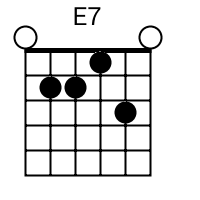
\includegraphics[width = 3cm]{../Akordy/e7.png}
% 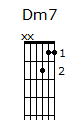
\includegraphics[width = 3cm]{../Akordy/dm7.png}

% 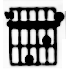
\includegraphics[width = 3cm]{../Akordy/esm7.png}
% 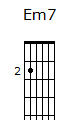
\includegraphics[width = 3cm]{../Akordy/em7.png}



\end{minipage}
}
\setcounter{Slokočet}{0}
\end{song}

\newpage
\addcontentsline{toc}{section}{Vlajky vlají}\begin{song}{title=\centering Vlajky vlají \\\normalsize Mig 21  \vspace*{-0.3cm}}  %% sem se napíše jméno songu a autor
\moveright 2.4cm \vbox{      %Varianta č. 1  ---> Jeden sloupec zarovnaný na střed	
\begin{minipage}[t]{0.48\textwidth}\setlength{\parindent}{0.45cm}  %Varianta č. 2 --> Dva sloupce

\sloka 
  Dobíhám ^{Dmi{\color{white}\_}}tramvaj
  
  \phantom{.}

  z kopce na Petřín

  a ty jedeš ^{Ami}v ní,

  v ^{{\color{white}\_\_}B}tramvaji.

  Koukneš se ^{E}ven,

  ^{C{\color{white}\_\_}}trolej ^{{\color{white}\_\_\_\_}Dmi}zajiskří.

\sloka
  Dobíhám tramvaj

  z kopce na Petřín

  a ty jedeš v ní,

  v tramvaji.

  Ta mění směr,

  kvér vystřelí.

\refren
  /: ^{Dmi}Na tramvaji vlajky vlají.


  ^{F}Mír volají, mír volají. :/

\sloka
  Zaklínám tramvaj,

  ať ještě zastaví

  a ty vystoupíš

  na chodník

  a pro šeřík 

  si chtít budeš jít.

\sloka
  Zaklínám tramvaj,

  ať ještě zastaví

  a ty vystoupíš

  na chodník.

  Ozve se křik, 

  jiskry padají.

\refren

  /: ^{Dmi}Mír ^{C\,\,F}volají. :/

\end{minipage}\begin{minipage}[t]{0.48\textwidth}\setlength{\parindent}{0.45cm}\vspace*{0.55cm}  % V případě varianty č.2 jde odsud text do pravé části

\sloka
  Začíná jaro

  nad Prahou, nad Plzní.

  Válka odezní,

  vyšumí.

  Nastane mír,

  osvobození.

\sloka
  Chtěl jsem jet s tebou

  noční tramvají -- ale 

  padám do křoví

  na šeřík.

  A v tom ten keř 

  tebou zavoní.

\refren 

  /: ^{Dmi}Mír ^{C\,\,F}volají. :/
  
  /: ^{Dmi}Mír ^{C\,\,F}volají. :/


\end{minipage}
}
\setcounter{Slokočet}{0}
\end{song}


\newpage
\addcontentsline{toc}{section}{Vlasy}\begin{song}{title=\centering Vlasy\\\normalsize Pokáč \vspace*{-0.3cm}}  %% sem se napíše jméno songu a autor
\moveright \stred \vbox{      %Varianta č. 1  ---> Jeden sloupec zarovnaný na střed	

\sloka 
	^{Ami}Občas si ^{F}říkám, jaký ^{G}by bylo ^{Ami}asi

	^{Ami}Probudit se ve ^{F}světě, kde ^{E}bych měl vlasy.

	Jestli by život nebyl lepší než 

	Ve světě, kde mám pleš.

\sloka
	Každý ráno bych si hezky rozčís ofinu
	
	Místo, abych aplikoval mast na lysinu.

	A holky v baru by třeba jednou tykaly
	
	A třeba mi i jinam než na lebku sahaly OU!

\sloka
	Občas si říkám, jaký by bylo asi
	
	Probudit se ve světě, kde bych měl vlasy.
	
	Jestli by život nebyl lepší než 
	
	Ve světě, kde mám pleš.

\sloka
	A dárkový set s šamponem by mě neurážel
	
	A světlo blesku na všech fotkách bych neodrážel
	
	A nemusel bych na bradě furt pěstovat porost,
	
	Abych dokázal, že mám pořád vlasů dost	
	
	A přitom vypadat, jak kretén.

\sloka
	Občas si říkám, jaký by bylo asi
	
	Probudit se ve světě, kde bych měl vlasy.
	
	Jasně, že mnohem lepší než mít pleš
	
	Ale nemůžeš mít všechno, co chceš.


}
\setcounter{Slokočet}{0}
\end{song}
\newpage
\addcontentsline{toc}{section}{Vlaštovky}\begin{song}{title=\predtitle\centering Vlaštovky \\\large Traband  \vspace*{-0.3cm}}  %% sem se napíše jméno songu a autor
\begin{centerjustified}

\sloka 
	^{Dmi\z}Každé jaro ^{Ami\z}z~velké dáli ^{B\z }vlaštovky k nám ^{F\z }přilétaly,

	^{Dmi\z }někdy až ^{C\z }dovnitř do ^{\z Ami}stavení.

	^{Dmi}Pod střechou se ^{Ami\z }uhnízdily a ^{B\z }lidé, kteří uvnitř ^{F\z }žili,
	
	^{Dmi\z }rozuměli ^{C\z }jejich ^{\z Ami}švitoření.


\sloka 
	O dalekých krajích, hlubokých mořích, divokých řekách,

	o vysokých horách, které je nutné přelétnout,

	o nebeských stezkách, zářících hvězdách, o cestách domů,

	o korunách stromů, kde je možné odpočinout.


\sloka 
	Jsme z míst, která jsme zabydlili,

	z hnízd, která jsme opustili,

	z cest, které končí na břehu.

	Jsme z lidí i všech bytostí,

	jsme z krve, z masa, z kostí,

	jsme ze vzpomínek, snů a příběhů.


\sloka 
	Jsme jako ti ptáci, z papíru draci, létáme v mracích

	a pak se vracíme zpátky tam, kde připoutaní jsme.

	Jsme lidské bytosti z masa a kostí, jsme jenom hosti

	na tomhle světě -- přicházíme, odcházíme.


\sloka 
	A chceme mít jisto, že někde je místo, že někde je hnízdo,

	odkud jsme přišli a kam zas potom půjdeme spát,

	že někde je domov, že někde je hnízdo, útulno čisto,

	že někde je někdo, kdo čeká na nás, na návrat.


\sloka 
	Tam v dalekých krajích, v hlubokých mořích, v divokých řekách,

	ve vysokých horách, které je nutné přelétnout.

	Tam v nebeských stezkách, v zářících hvězdách, na cestách domů,

	v korunách stromů, kde je možné odpočinout.

\end{centerjustified}
\setcounter{Slokočet}{0}
\end{song}
\newpage
\addcontentsline{toc}{section}{What Makes You Beautiful}%\documentclass[../main.tex]{subfiles}

\begin{song}{title=\centering What Makes You Beautiful \\\normalsize One Direction  \vspace*{-0.3cm}}  %% sem se napíše jméno songu a autor
\moveright 3cm \vbox{      %Varianta č. 1  ---> Jeden sloupec zarovnaný na střed	


\sloka
You're ^{\,\,D}insecure ^{G} 

Don't know what ^{A}for 

You're turning ^{D{\color{white}\_}}heads when you ^{G{\color{white}\_}}walk through the ^{A{\color{white}\_}}door 

Don't need make ^{D}up 

^{G}To cover ^{A}up 

Being the ^{D}way that you ^{G}are is ^{A}enough 

%\moveright -0.2cm \vbox{\ssloka \textbf{R\textsubscript{1}:}
^{D{\color{white}\_\_\_}}Everyone ^{G\,\,}else in the ^{A{\color{white}\_}}room can see it 

^{D{\color{white}\_\_\_}}Everyone ^{G}else but ^{A}you
 
%\moveright -0.2cm \vbox{\ssloka \textbf{R\textsubscript{2}:}
Baby you ^{D{\color{white}\_}}light up my ^{G{\color{white}\_}}world like ^{A}nobody else 

The way that ^{D}you flip your ^{G}hair gets me ^{A{\color{white}\_\_\_\_}}overwhelmed 

But you when ^{D{\color{white}\_}}smile at the ^{G{\color{white}\_\_}}ground it ain't ^{A}hard to tell 

You don't ^{\,\,\,D (Hmi)}know oh ^{G}oh

^{A}You don't know you're ^{{\color{white}\_\_}D}beautiful 

%\moveright -0.2cm \vbox{\ssloka \textbf{R\textsubscript{3}:}
If only ^{A}you saw what ^{H}I can see 

You'll ^{D{\color{white}\_\_\_\_}}understand why I ^{G}want you so ^{A{\color{white}\_\_\_\_}}desperately 

Right now I'm ^{D{\color{white}\_\_\_}}looking at ^{G}you and I ^{A}can't believe 

You don't ^{\,\,\,D (Hmi)}know oh ^{G}oh

^{A}You don't know you're ^{{\color{white}\_\_}D}beautiful oh - ^{G}oh  

But ^{A}that's what makes you ^{{\color{white}\_\_}D}beautiful 

\sloka
So c-come on 

You got it wrong

To prove I'm right I put it in a song  

I don't why

You're being shy

And turn away when I look into your eyes 


}
\newpage
\moveright 3cm \vbox{      %Varianta č. 1  ---> Jeden sloupec zarovnaný na střed	

%\moveright -0.2cm \vbox{\ssloka \textbf{R\textsubscript{1}:}
^{D{\color{white}\_\_\_}}Everyone ^{G\,\,}else in the ^{A{\color{white}\_}}room can see it 

^{D{\color{white}\_\_\_}}Everyone ^{G}else but ^{A}you
 
%\moveright -0.2cm \vbox{\ssloka \textbf{R\textsubscript{2}:}
Baby you ^{D{\color{white}\_}}light up my ^{G{\color{white}\_}}world like ^{A}nobody else 

The way that ^{D}you flip your ^{G}hair gets me ^{A{\color{white}\_\_\_\_}}overwhelmed 

But you when ^{D{\color{white}\_}}smile at the ^{G{\color{white}\_\_}}ground it ain't ^{A}hard to tell 

You don't ^{\,\,\,D (Hmi)}know oh ^{G}oh

^{A}You don't know you're ^{{\color{white}\_\_}D}beautiful 

%\moveright -0.2cm \vbox{\ssloka \textbf{R\textsubscript{3}:}
If only ^{A}you saw what ^{H}I can see 

You'll ^{D{\color{white}\_\_\_\_}}understand why I ^{G}want you so ^{A{\color{white}\_\_\_\_}}desperately 

Right now I'm ^{D{\color{white}\_\_\_}}looking at ^{G}you and I ^{A}can't believe 

You don't ^{\,\,\,D (Hmi)}know oh ^{G}oh

^{A}You don't know you're ^{{\color{white}\_\_}D}beautiful oh - ^{G}oh  

But ^{A}that's what makes you ^{{\color{white}\_\_}D}beautiful 

\sloka
^{D}Nana Nana ^{G}Nana Nana  ^{A}Nana Nana na

^{D}Nana Nana ^{G}Nana Nana  ^{A}Nana Nana na 

^{G}Nana Nana^{A} Nana Nana   

%\moveright -0.2cm \vbox{\ssloka \textbf{R\textsubscript{2}:}

%\moveright -0.2cm \vbox{\ssloka \textbf{R\textsubscript{2}:}

%\moveright -0.2cm \vbox{\ssloka \textbf{R\textsubscript{3}:}
 

}
\setcounter{Slokočet}{0}
\end{song}
\newpage
\addcontentsline{toc}{section}{What Shall We Do With the Drunken Sailor}\begin{song}{title=\centering What Shall We Do With the Drunken Sailor \\\normalsize   \vspace*{-0.3cm}}  %% sem se napíše jméno songu a autor
\moveright 4.8cm \vbox{      %Varianta č. 1  ---> Jeden sloupec zarovnaný na střed	

\sloka 
	^{Ami}What shall we do with a drunken sailor 
	
	^{G}what shall we do with a drunken sailor 

	^{Ami}what shall we do with a drunken sailor 
	
	early ^{Emi}in the ^{Ami}morning? 


\refren
	
	^{Ami}Hooray and up she rises ^{G}hooray and up she rises 
	
	^{Ami}hooray and up she rises early ^{Emi}in the ^{Ami}morning. 


\sloka
	Put him in the longboat till he's sober 
	
	put him in the longboat till he's sober 
	
	put him in the longboat till he's sober 

	early in the morning. 


\refren

\sloka
	Pull out the plug and wet him all over 
	
	pull out the plug and wet him all over 
	
	pull out the plug and wet him all over 
	
	early in the morning. 

\refren

}
\setcounter{Slokočet}{0}
\end{song}


\begin{figure}[h]
\centering
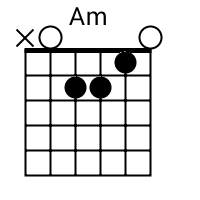
\includegraphics[scale=1.5]{../Akordy/am.png}
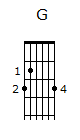
\includegraphics[scale=1.5]{../Akordy/g.png}
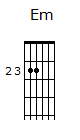
\includegraphics[scale=1.5]{../Akordy/em.png}
\end{figure}
\newpage
\addcontentsline{toc}{section}{Zatanči}\begin{song}{title=\centering Zatanči \\\normalsize Jaromír Nohavica  \vspace*{-0.3cm}}  %% sem se napíše jméno songu a autor
\moveright \stred \vbox{      %Varianta č. 1  ---> Jeden sloupec zarovnaný na střed	

\sloka
^{Emi G}Zatanči, má milá, ^{D{\color{white}\_\_}}zatanči ^{Emi}pro mé oči,

^{{\color{white}\_\_}G}zatanči a vetkni nůž ^{D}do mých ^{Emi}zad.

Ať tvůj ^{G}šat, má milá, ať ^{D}tvůj šat ^{Emi}na zemi skončí,

ať tvůj ^{G}šat, má milá, ^{D}rázem je ^{Emi}sňat.

\refren
^{Emi G}Zatanči, jako se ^{D{\color{white}\_}}okolo ^{Emi\,\,}ohně tančí,

^{{\color{white}\_\_}G}zatanči jako ^{D{\color{white}\_\_}}na\,\,vodě ^{Emi}loď,

^{{\color{white}\_\_}G}zatanči jako to ^{D}slunce ^{Emi}mezi pomeranči,

^{{\color{white}\_\_}G}zatanči, a ^{D}pak ke mně ^{Emi}pojď.

\phantom{.}

\textbf{Mezihra}

\sloka
Polož dlaň, má milá, polož dlaň na má prsa,

polož dlaň nestoudně na moji hruď.

Obejmi, má milá, obejmi moje bedra,

obejmi je pevně a mojí buď.

\refren

\phantom{.}

\textbf{Mezihra}

\sloka
Nový den než začne, má milá, nežli začne,

nový den než začne, nasyť můj hlad.

Zatanči, má milá, pro moje oči lačné,

zatanči a já budu ti hrát.

\refren

\refren
}
\setcounter{Slokočet}{0}
\end{song}
\newpage
\addcontentsline{toc}{section}{My pluli}\documentclass[../main.tex]{subfiles}


\chapter{My Pluli Dál A Dál }
\noindent\hspace{0.3\linewidth}\begin{minipage}{0.8\linewidth}
\begin{song}{title=Pangajó}

\begin{verse}[numbered]
 	My pluli ^{G}dál a dál v zelené ^{D}lesy, 
                               
    kde vlnka s vlnkou ^{D7}slaví své ^{G}plesy, 
                       
    my pluli dál a dál ^{G7}v zelený ^{C}háj, 
                               
    my pluli ^{G}dál a dál v ^{D} zelený ^{G}háj.
\end{verse}
\begin{verse}[numbered]
	Loďka je malá, vesla jsou krátký, 
	
    poplujem hoši, poplujem zpátky, 
    
  /:či máme plouti dál v zelený háj. :/ 
\end{verse}
\begin{verse}[numbered]
	 My pluli dál a dál v rákosí tmavé, 
	 
    kde rybka s rybkou spolu si hraje, 
    
  /:my pluli dál a dál v zelený háj. :/
\end{verse}
\begin{verse}[numbered]
	My pluli dál a dál s malou lodičkou, 
	
    my pluli dál a dál tichou vodičkou, 
    
    my pluli dál a dál v neznámý svět, 
    
    my pluli dál a dál a nikdy zpět. 
\end{verse}
\end{song}
\end{minipage}
\newpage






\newgeometry{top=1cm, bottom = 1cm, left = 1cm, right = 1cm}
\thispagestyle{empty}
\begin{figure}[h]
\centering
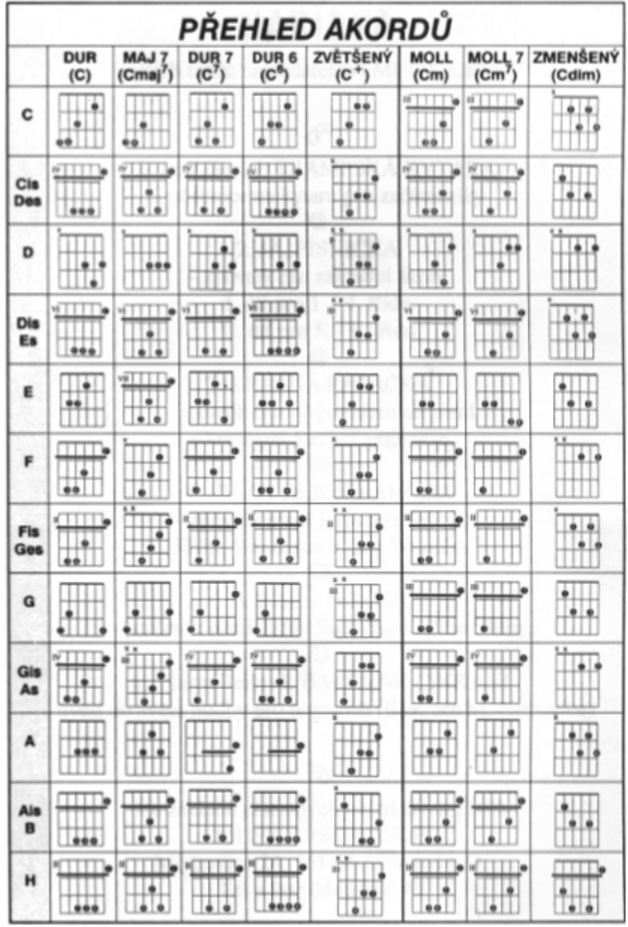
\includegraphics[height=\textheight]{../Akordy/akordymale.pdf}
\end{figure}



\end{document}

